%%%%%%%%%%%%%%%%%%%%%%%%%%%%%%%%%%%%%%%%%%%%
% Author: Bijesh Mishra              %
% License: GNU General Public License v3.0 %
%%%%%%%%%%%%%%%%%%%%%%%%%%%%%%%%%%%%%%%%%%%%

\documentclass[11pt]{beamer}
%The full list of themes is:: AnnArbor, Antibes, Bergen, Berkeley, Berlin, CambridgeUS, Copenhagen, Darmstadt, Dresden, Frankfurt,  Goettingen, Hannover, Ilmenau, JuanLesPins,  Luebeck, Madrid, Malmoe, Marburg, Montpellier, PaloAlto, Pittsburgh, Rochester, Singapore, Szeged, Warsaw, boxes, default
\usetheme{Singapore} % Use this with different color fot this presentation.
\usefonttheme[]{serif}
% \usetheme{Dresden} % I like this. Similar to Ilmenau. Szeged
% \usetheme{Copenhagen}
% \usetheme{Warsaw} % Same as Luebeck, Malmoe
% The full list of color themes is: default, albatross, beaver, beetle, crane, dolphin, dove, fly, lily, orchid, rose, seagull, seahorse, whale, wolverine
% \usecolortheme{}
\usecolortheme{seagull} % with  Dresden.
\usepackage{graphicx}
\usepackage{fancyhdr}
\usepackage{hyperref}
\usepackage{anyfontsize}
\usepackage{tcolorbox}
\usepackage[utf8]{inputenc}
\usepackage{colortbl}
\newcommand{\RowColor}{\rowcolor{gray!60}}
\usepackage{adjustbox}
\usepackage{tikzsymbols}
\usepackage{array}
\usepackage{amsmath}
\usepackage{listings}
\usepackage{fontawesome5}
\usepackage{xcolor}

\lstset
{
	language={[LaTeX]TeX},
	frame=single,
	framesep=\fboxsep,
	framerule=\fboxrule,
	rulecolor=\color{black},
	xleftmargin=\dimexpr\fboxsep+\fboxrule,
	xrightmargin=\dimexpr\fboxsep+\fboxrule,
	breaklines=true,
	basicstyle=\small\tt,
	keywordstyle=\color{blue} \sf,
	commentstyle=\color{purple!100},
	backgroundcolor=\color{gray!10},
	tabsize=2,
	columns=flexible,
}

\graphicspath{ {./Images/} }
\usenavigationsymbolstemplate{}
\vspace{-2cm}
\title{\bf Dissecting Peer-reviewed Paper Publishing Process}
\vspace{0.2cm}
\subtitle{Ethics on Research and Publication Series}
\author{\bf Bijesh MISHRA, Ph.D. }
\institute{\color{blue}
\faIcon{envelope} \href{mailto: bzm0094@auburn.edu}{bzm0094@auburn.edu}
\faIcon{envelope} \href{mailto: bijesh.mishra@okstate.edu}{bijesh.mishra@okstate.edu} \\
\faIcon{map-marker-alt} 
Auburn University, Auburn, AL \\
{\color{blue}\href{https://bijeshmishra.com/}{\faIcon{globe} https://bijeshmishra.com/}} \\
}
\date{July 22, 2023} 
%%%%%%%%%%%%%%%%%%%%%%

%%%%%%%%%%%%%%%%%%%%%%
\begin{document}
\begin{frame}
	{\frame{\titlepage}}
\end{frame}
%%%%%%%%%%%%%%%%%%%%%%%

%%%%%%%%%%%%%%%%%%%%%%%
\subsection*{Resource Person Introduction}
\begin{frame}{}
    \centering 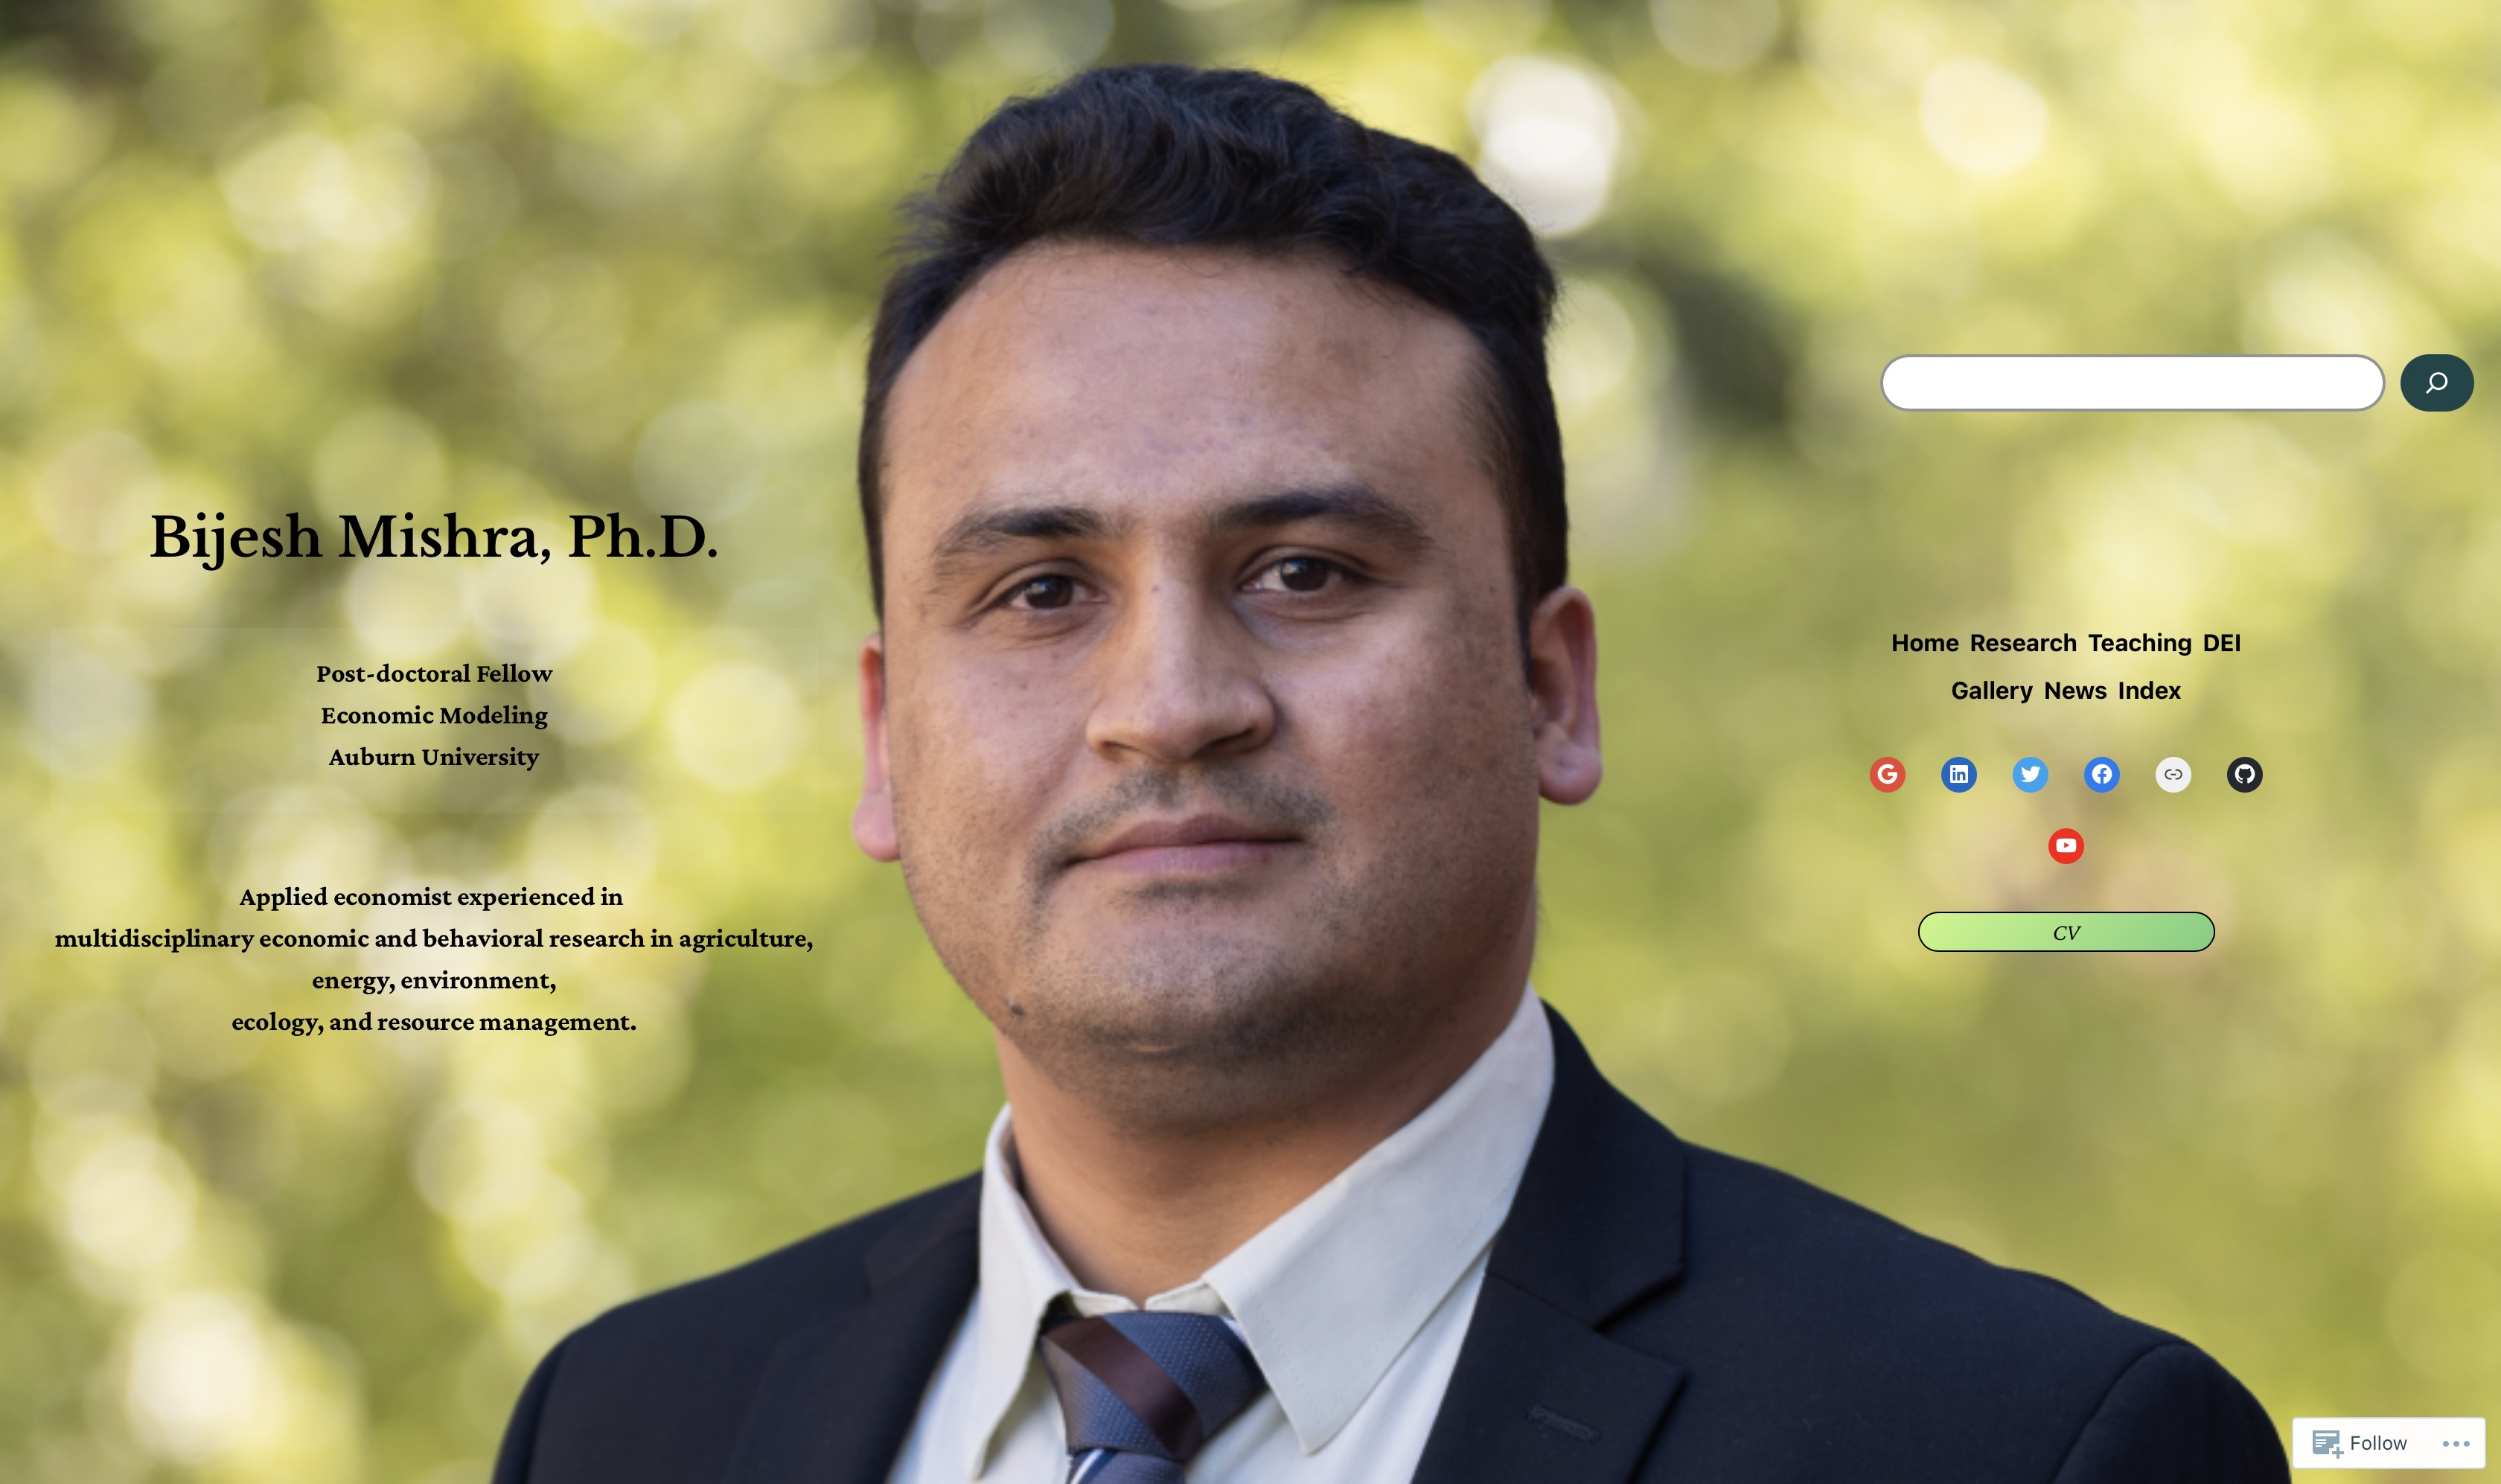
\includegraphics[width = \textwidth, height = 0.8\textheight]{Images/Website.jpeg}
    \vspace{0.3cm}
    \centering {\color{blue}\href{https://twitter.com/BijuBjs}{\faIcon{twitter} BijuBjs}}
    \hspace{0.2cm}
    \centering {\color{blue}\href{https://www.facebook.com/BMishraPhD}{\faIcon{facebook} BMishraPhD}} 
    \hspace{0.2cm}
    \centering {\color{blue}\href{https://www.linkedin.com/in/bijubjs/}{\faIcon{linkedin} BijuBjs}} \\
    \centering {\color{blue}\href{https://bijeshmishra.com/}{\faIcon{globe} https://bijeshmishra.com/}}
\end{frame}   
%%%%%%%%%%%%%%%%%%%%%%

%%%%%%%%%%%%%%%%%%%%%%
\begin{comment}
\begin{frame}{Table of Content}
	\tableofcontents
\end{frame}    
\end{comment}
%%%%%%%%%%%%%%%%%%%%%

\section{Content}
%%%%%%%%%%%%%%%%%%%%%
\subsection{Content}
\begin{frame}{Content of Presentation}
\begin{itemize}
\vspace{0.5 cm}
  \item \textbf{Part I:} Predatory vs peer-reviewed publication process.
  \vspace{1 cm}
  \item \textbf{Part II:} Dissecting peer-reviewed papers.
\end{itemize}
\end{frame}
%%%%%%%%%%%%%%%%%%%%%

\begin{comment} 
\section{Information}
%%%%%%%%%%%%%%%%%%%%%
\subsection{Source of Information}
\begin{frame}{Source of Information}
\begin{itemize}
  \item \textbf{General information sources:} YouTube videos, personal communications, daily news, movies, TV shows etc.
  \vspace{0.10 cm}
  %\pause

  \item \textbf{General articles:} newsletters, newspaper, blogs, etc.
  \vspace{0.10 cm}
  %\pause

  \item \textbf{Non peer reviewed scientific articles:} dissertation, thesis, preprints, conference proceedings, fact sheets etc.
  \vspace{0.10 cm}
  %\pause  

  \item {\color{blue}\textbf{\href{https://www.elsevier.com/reviewers/what-is-peer-review}{Peer reviewed}}} scientific articles: Scientific article reviewed by \textbf{expert in their respective field} to maintain \textbf{quality} and \textbf{validity} of published articles in scientific journals.
  \vspace{0.10 cm}
\end{itemize}
\end{frame}
\end{comment}
%%%%%%%%%%%%%%%%%%%%%
	
\section{Peer Review}
%%%%%%%%%%%%%%%%%%%%%
\begin{frame}{Peer Review Process}
\begin{itemize}
    \item {\color{blue}\textbf{\href{https://www.elsevier.com/reviewers/what-is-peer-review}{Peer review}}} process involves several steps and takes time.
\end{itemize}
%\pause
\centering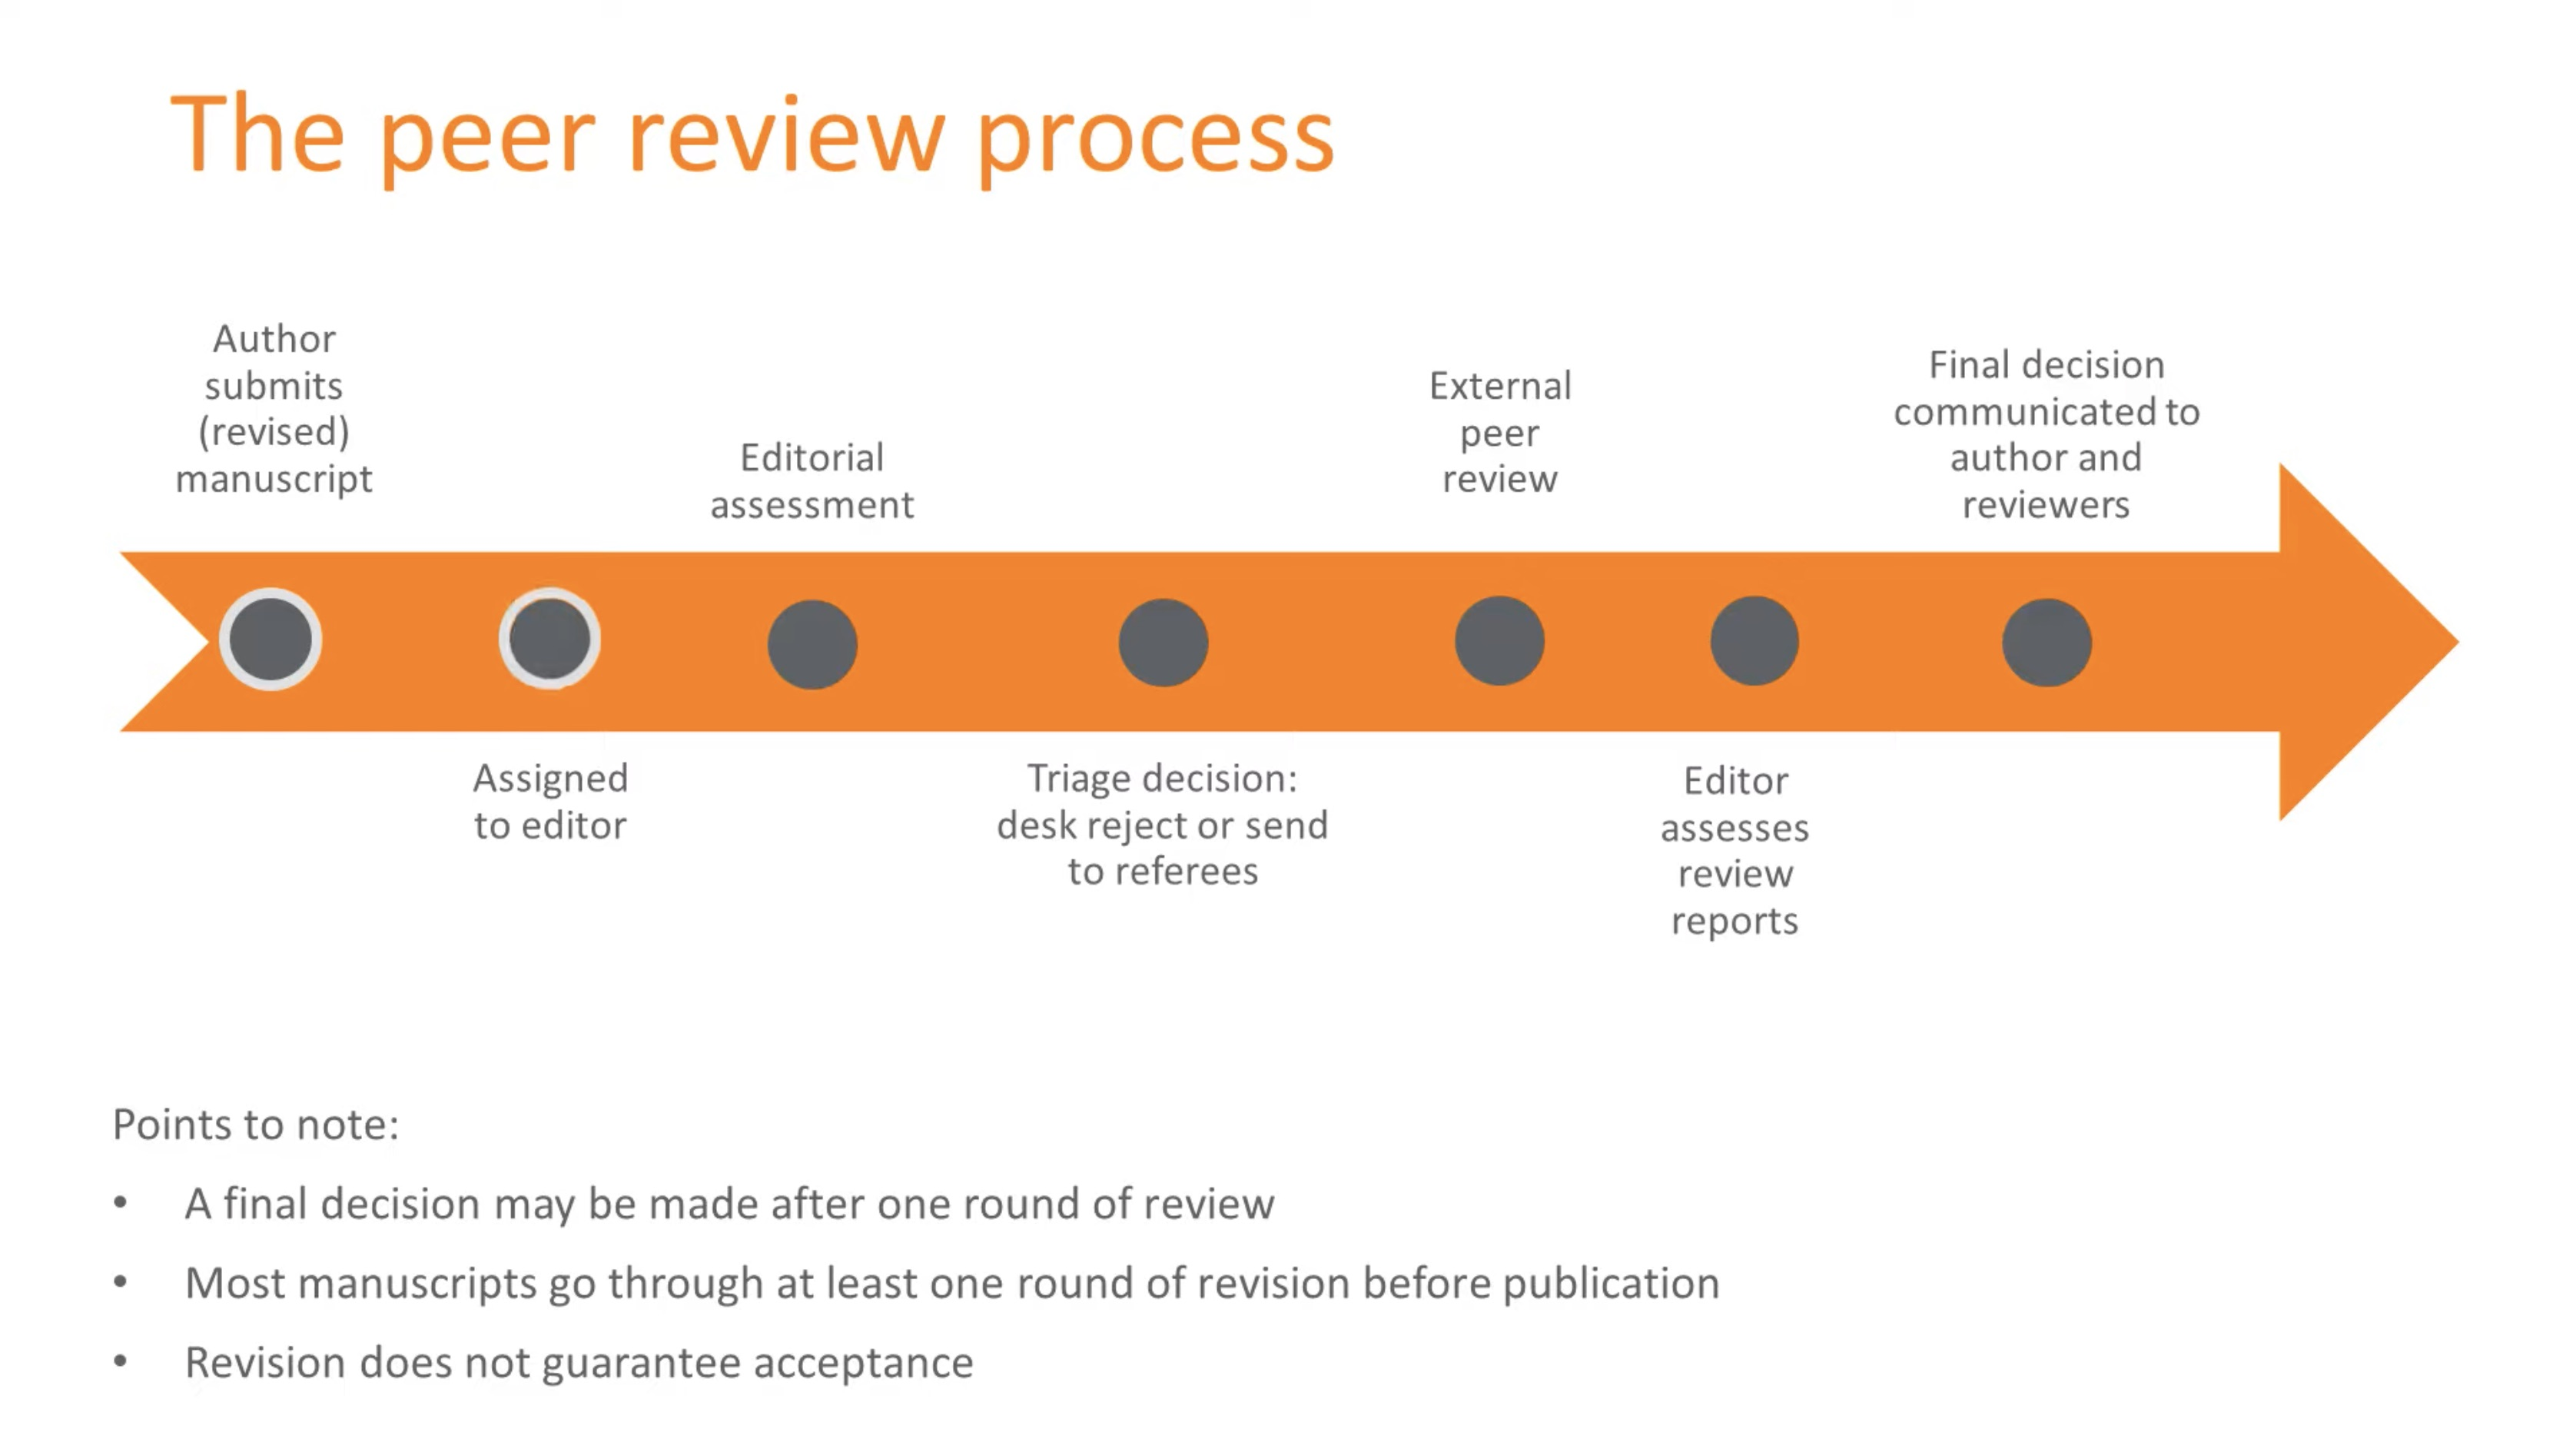
\includegraphics[width = \textwidth, height = 0.75\textheight]{Images/Peer review process.jpeg}
\end{frame}
%%%%%%%%%%%

%%%%%%%%%%%
\begin{frame}{Peer Review Process}
\begin{itemize}
    \item May ask you to submit sample or full dataset, code, copies of lab notebooks etc. during the review process.
    \vspace{0.10 cm}
    %\pause
    
    \item Publishing peer reviewed scientific paper is often {\color{magenta}\textbf{FREE}} and may require you to sign copyright transfer agreement.
    \vspace{0.10 cm}
    %\pause
    
    \item {\color{red}\textbf{EXCEPTION:}} Open source journals where you may have to {\color{brown}\textbf{pay publication fee}}: {\color{green}PLAYGROUND} for predatory journals.
    \vspace{0.10 cm}
    
    \item {\color{red}\textbf{EXCEPTION:}} Contract with publisher on your own terms and conditions.
\end{itemize}
\end{frame}
%%%%%%%%%%%

\section{Predatory Process}
%%%%%%%%%%%%%%%%%%%%%%%%%%%
\subsection{Predatory Process}
\begin{frame}{Predatory Process}
\begin{itemize}
	\smallskip
	\item Predominantly \textbf{prey} researchers around the world primarily from developing countries.
	\smallskip
	\item By soliciting manuscripts for a \textbf{nominal publication fee}.
	\smallskip
	\item \textbf{Without robust editorial service} or \textbf{peer review system}. 
	\smallskip
	\item Promising \textbf{fast track publication} in \textbf{a few days to weeks}.
    \smallskip
\end{itemize}
    {\color{blue}\href{https://www.sciencedirect.com/science/article/pii/S0363018821001389}{Mathew et al., 2022}}. Predatory Journals-The Power of the Predator Versus the Integrity of the Honest, \textit{Current Problems in Diagnostic Radiology}.
\end{frame}
%%%%%%%%%%%

\begin{comment}
%%%%%%%%%%%
\begin{frame}{Predatory Process: Recent Development}
	\centering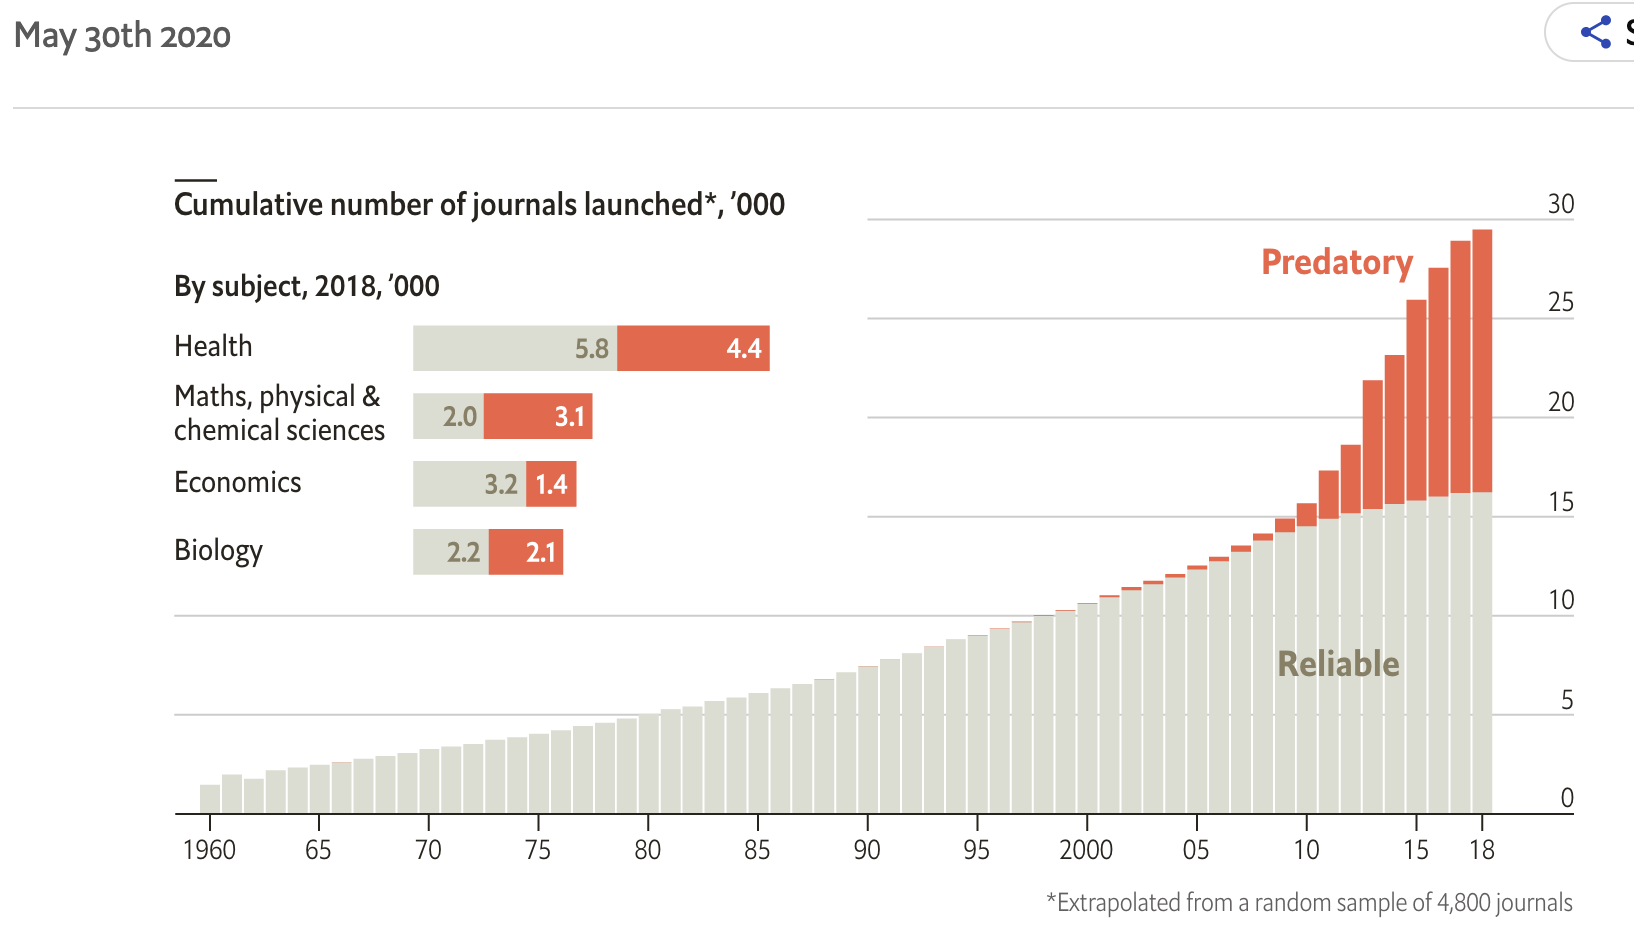
\includegraphics[width = \textwidth, height = 0.7\textheight]{Images/PredCount.png} \\
 How to spot dodgy academic journals, {\color{blue}\href{https://www.economist.com/graphic-detail/2020/05/30/how-to-spot-dodgy-academic-journals}{The Economist}}
\end{frame}
%%%%%%%%%%%    
\end{comment}

%%%%%%%%%%%
\begin{frame}{Predatory Process: Recent Development}
	\begin{itemize}
    \item Predatory publishing is getting worse: \textbf{fewer publishers but more journals} {\color{blue}\href{https://link.springer.com/article/10.1007/s12109-022-09888-z}{(Kendal and Linacre, 2022)}}.
    \smallskip\
    \item About \textbf{55\% of the authors published 1} and 35\% published 2–5 papers in predatory journals {\color{blue}\href{https://doi.org/10.1002/leap.1489}{(Frandsen, 2022)}}.
    \smallskip
    \item Initially, {\color{blue}{\href{https://www.linkedin.com/pulse/all-mdpi-journals-listed-predatory-christos-kontovas/}{all MDPI Journals}}} were listed as predatory by {\color{blue}\href{https://predatoryreports.org/home}{predatory reports}} which was {\color{blue}{\href{https://predatoryreports.org/news/f/list-of-all-mdpi-predatory-publications?blogcategory=MDPI}{revised}}} after MDPI {\color{blue}\href{https://www.mdpi.com/about/announcements/5482}{published an article}} criticizing their action.
    \smallskip
    \item Journal name has \textquotedblleft World\textquotedblright, \textquotedblleft international\textquotedblright, \textquotedblleft global\textquotedblright but ($\approx$) \textbf{no} information about publishers ({\color{blue}\href{https://www.nature.com/articles/495433a}{Butler, 2013}}){\color{red} !!!}.
    \smallskip
    \item How to spot dodgy academic journals, {\color{blue}\href{https://www.economist.com/graphic-detail/2020/05/30/how-to-spot-dodgy-academic-journals}{The Economist.}}
\end{itemize}
\end{frame}
%%%%%%%%%%%

%%%%%%%%%%%
\begin{frame}{Predatory Journals: No Definition, No Defence}
    \centering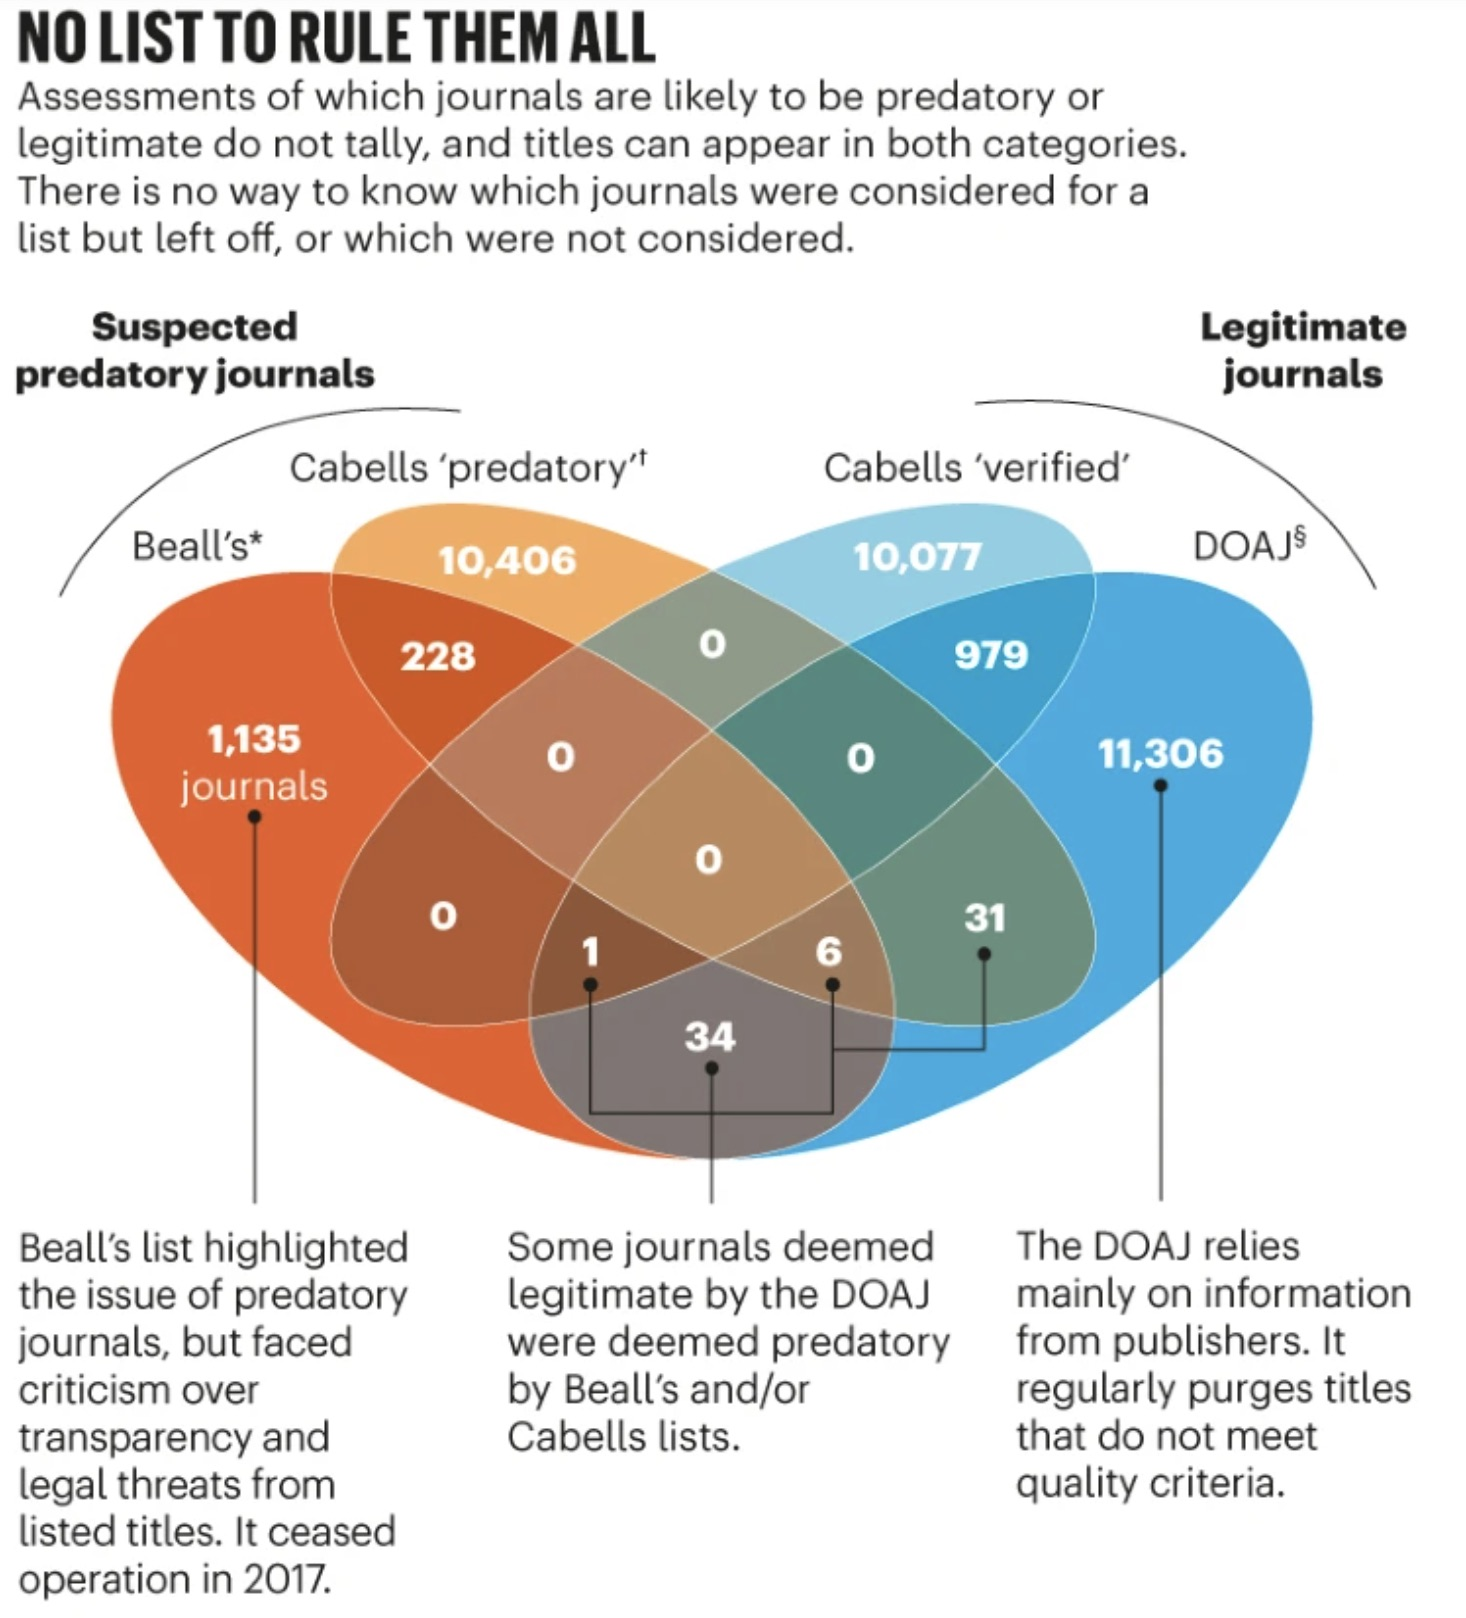
\includegraphics[width = 0.6\textwidth]{Images/Belles.jpeg}
\end{frame}
%%%%%%%%%%%

%%%%%%%%%%%
\begin{frame}{Why Researchers Publish in Predatory Journals?}
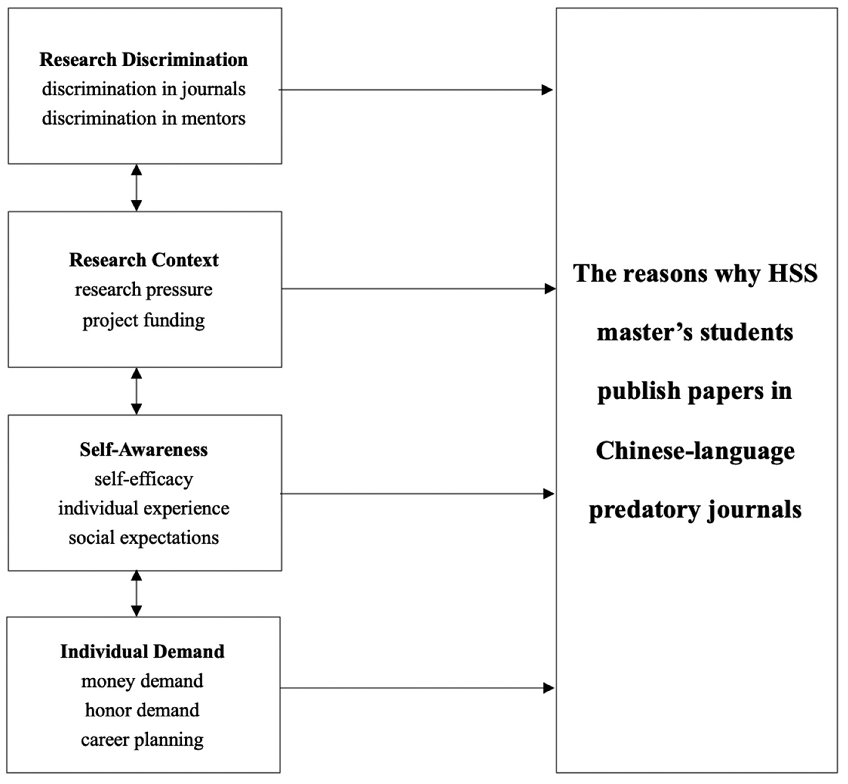
\includegraphics[width=0.6\textwidth]{WhyPred.png}%
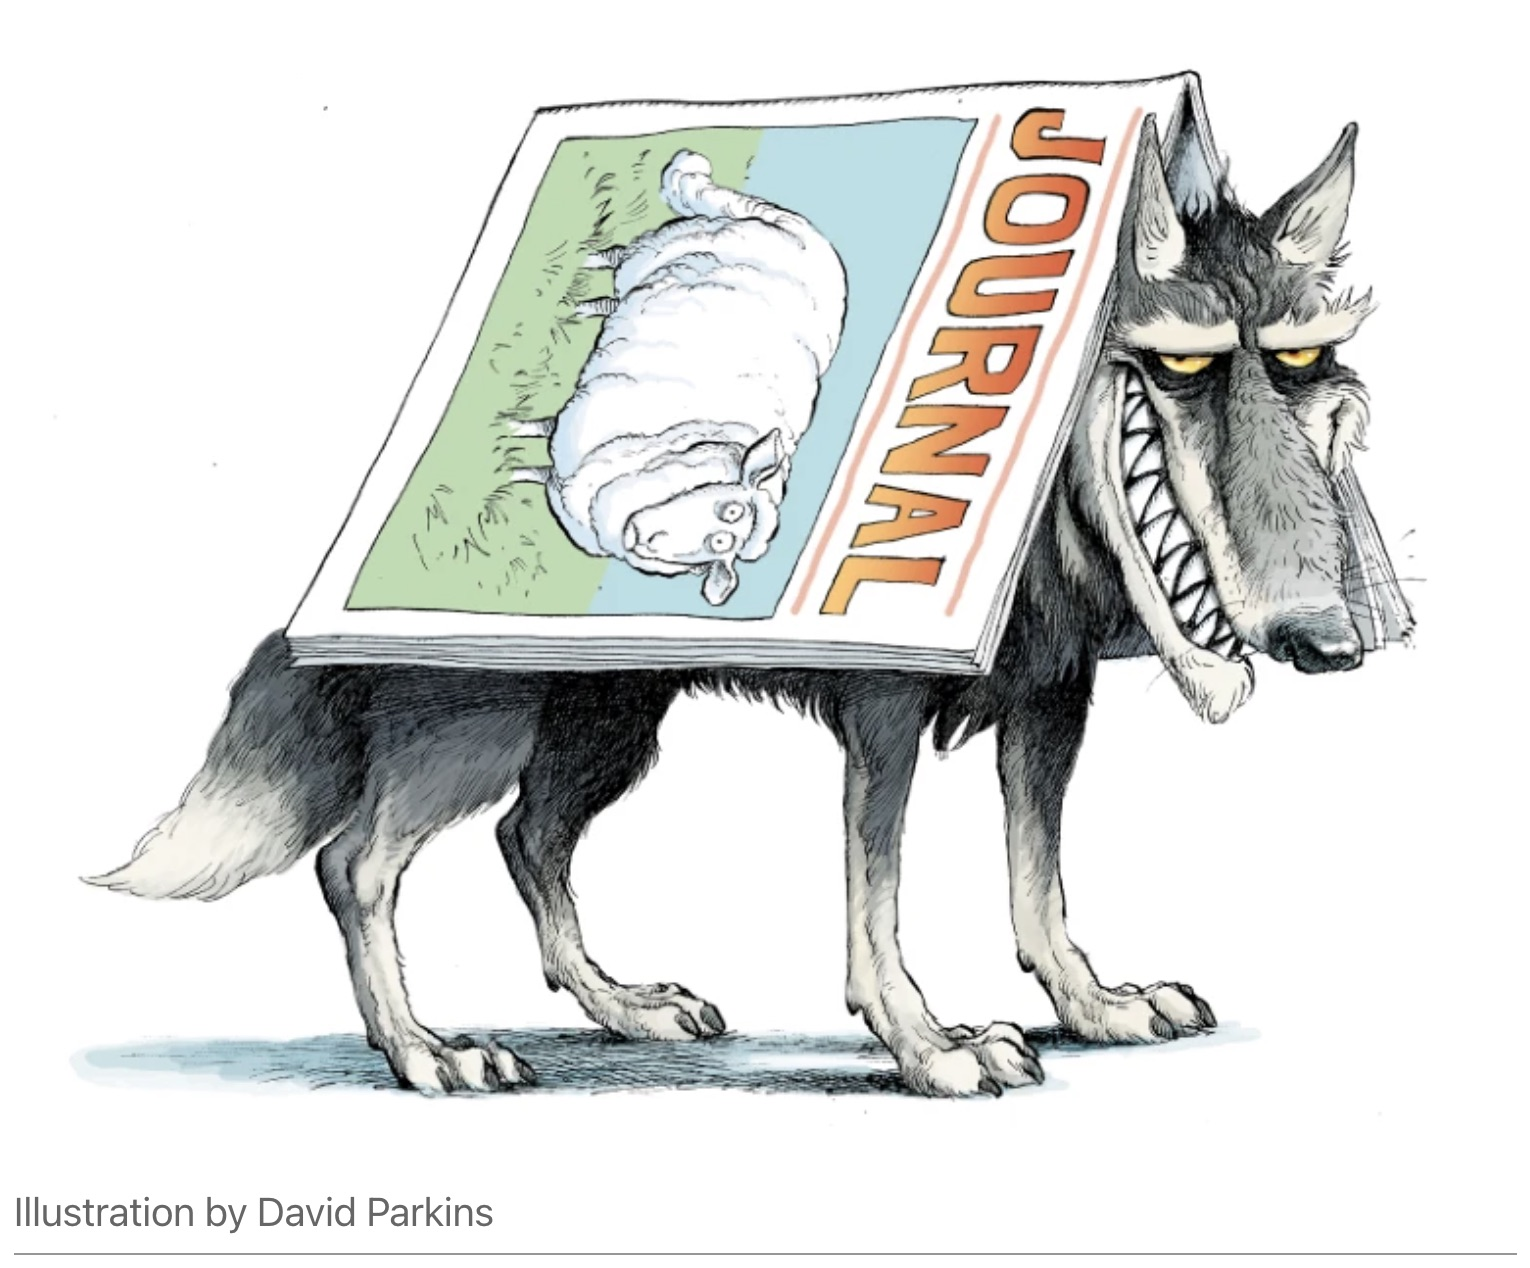
\includegraphics[width=0.4\textwidth]{Images/David.jpeg}
\centering{\color{blue}\href{https://doi.org/10.1080/08989621.2021.1960164}{Tang and Jia, 2023}} in \textit{Accountability in Research}
\end{frame}
%%%%%%%%%%%

%%%%%%%%%%%
\begin{frame}{Predatory Journal Invitation}
	\centering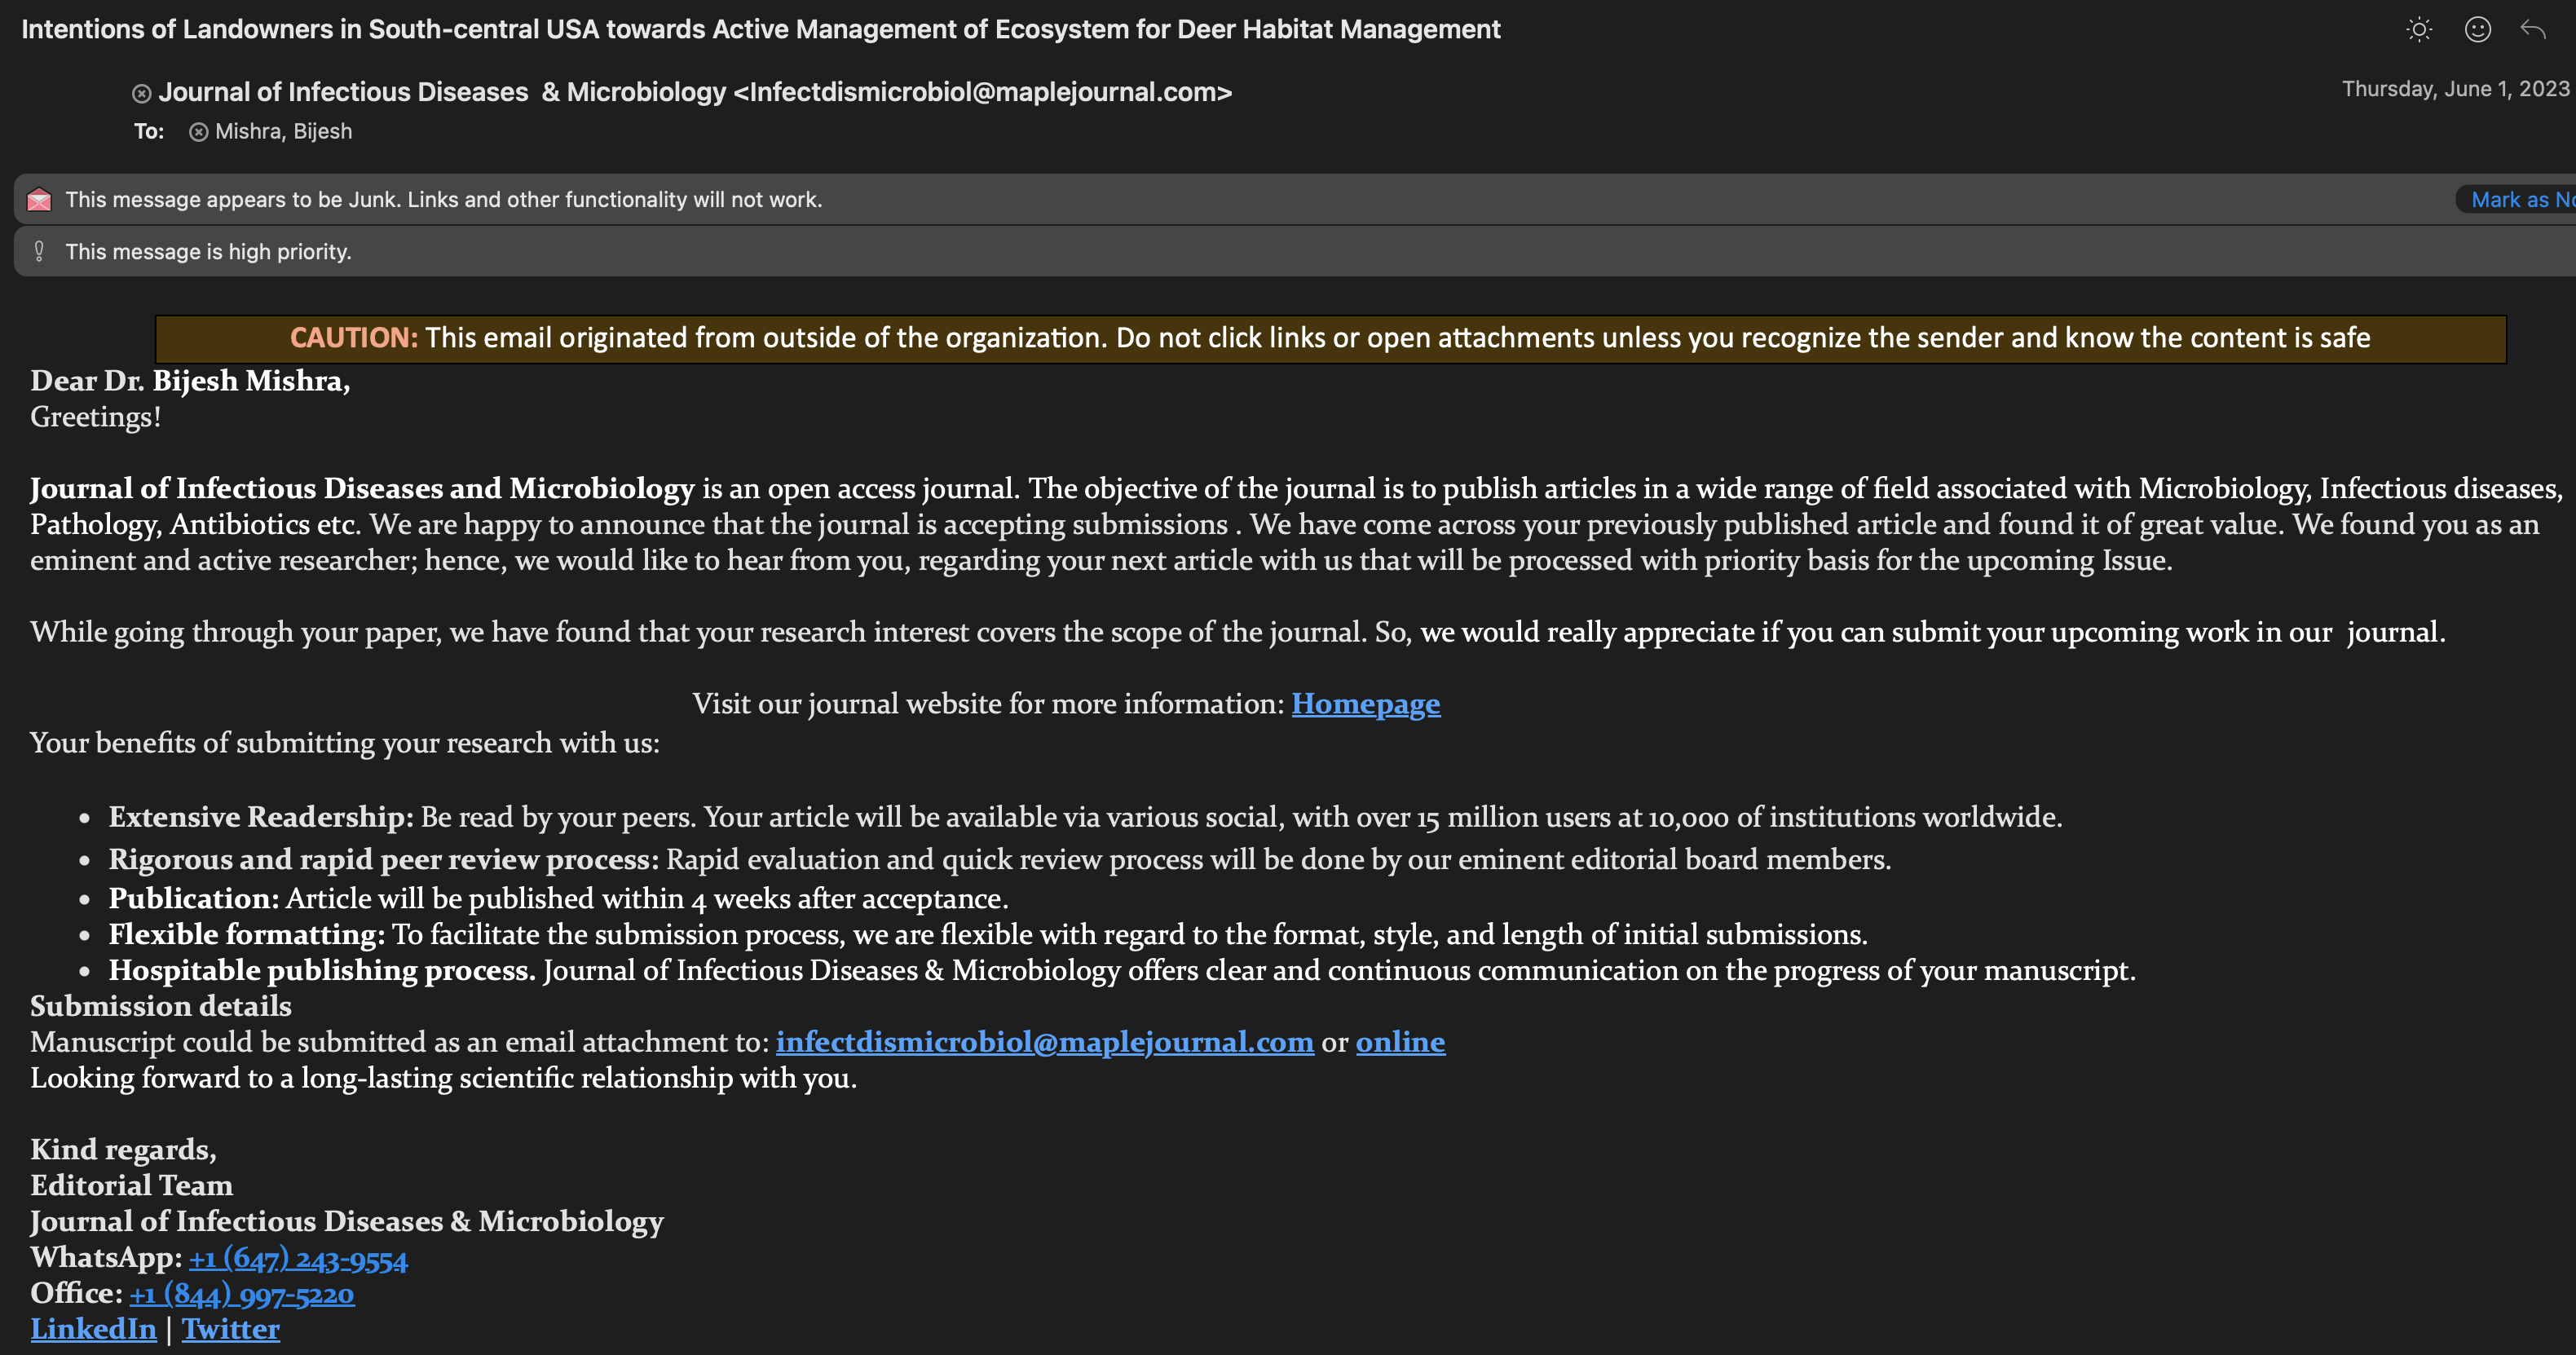
\includegraphics[width = \textwidth, height = 0.8\textheight]{Images/Pred Email.png} \\
 Figure: Invitation email from a predatory journal.
\end{frame}
%%%%%%%%%%%

%%%%%%%%%%%
\begin{frame}{Predatory Journal Invitation}
	\centering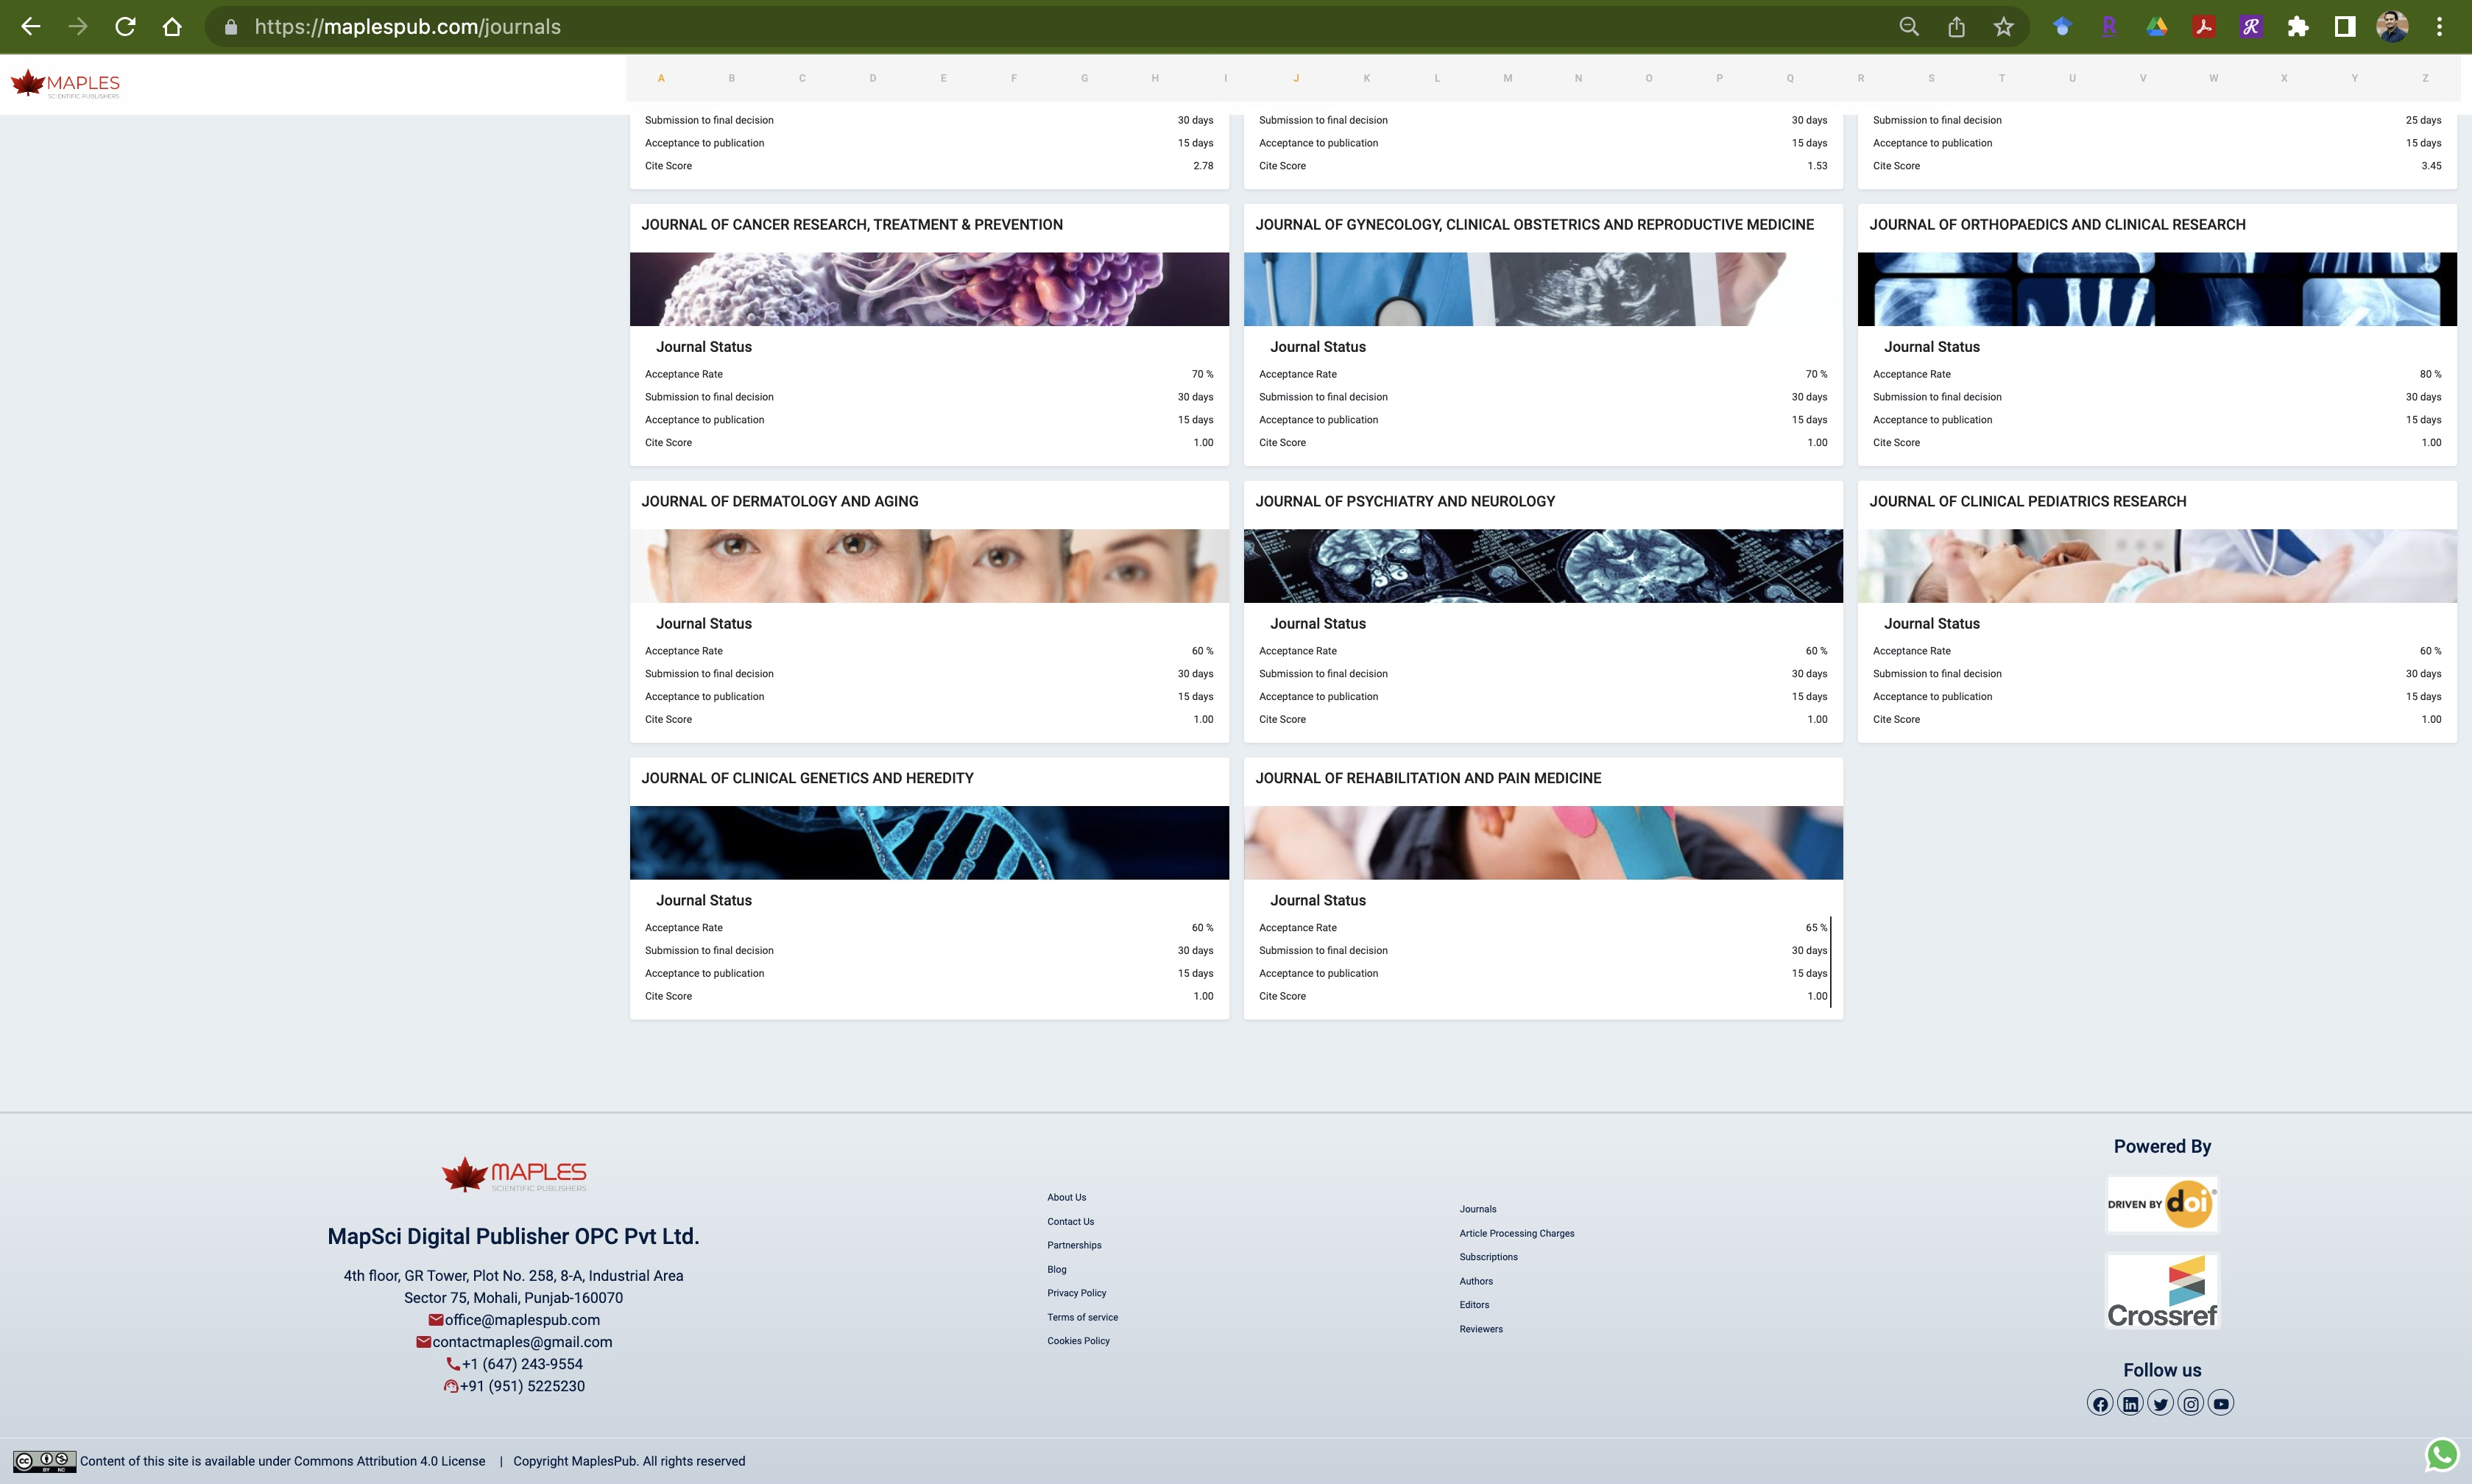
\includegraphics[width = \textwidth, height = 0.8\textheight]{Images/Maples.jpeg} \\
 Figure: Maples (Not listed in predatory publisher's list).
\end{frame}
%%%%%%%%%%%

%%%%%%%%%%%
\begin{frame}{Identifying: Predatory Journals Spectrum}
	\centering 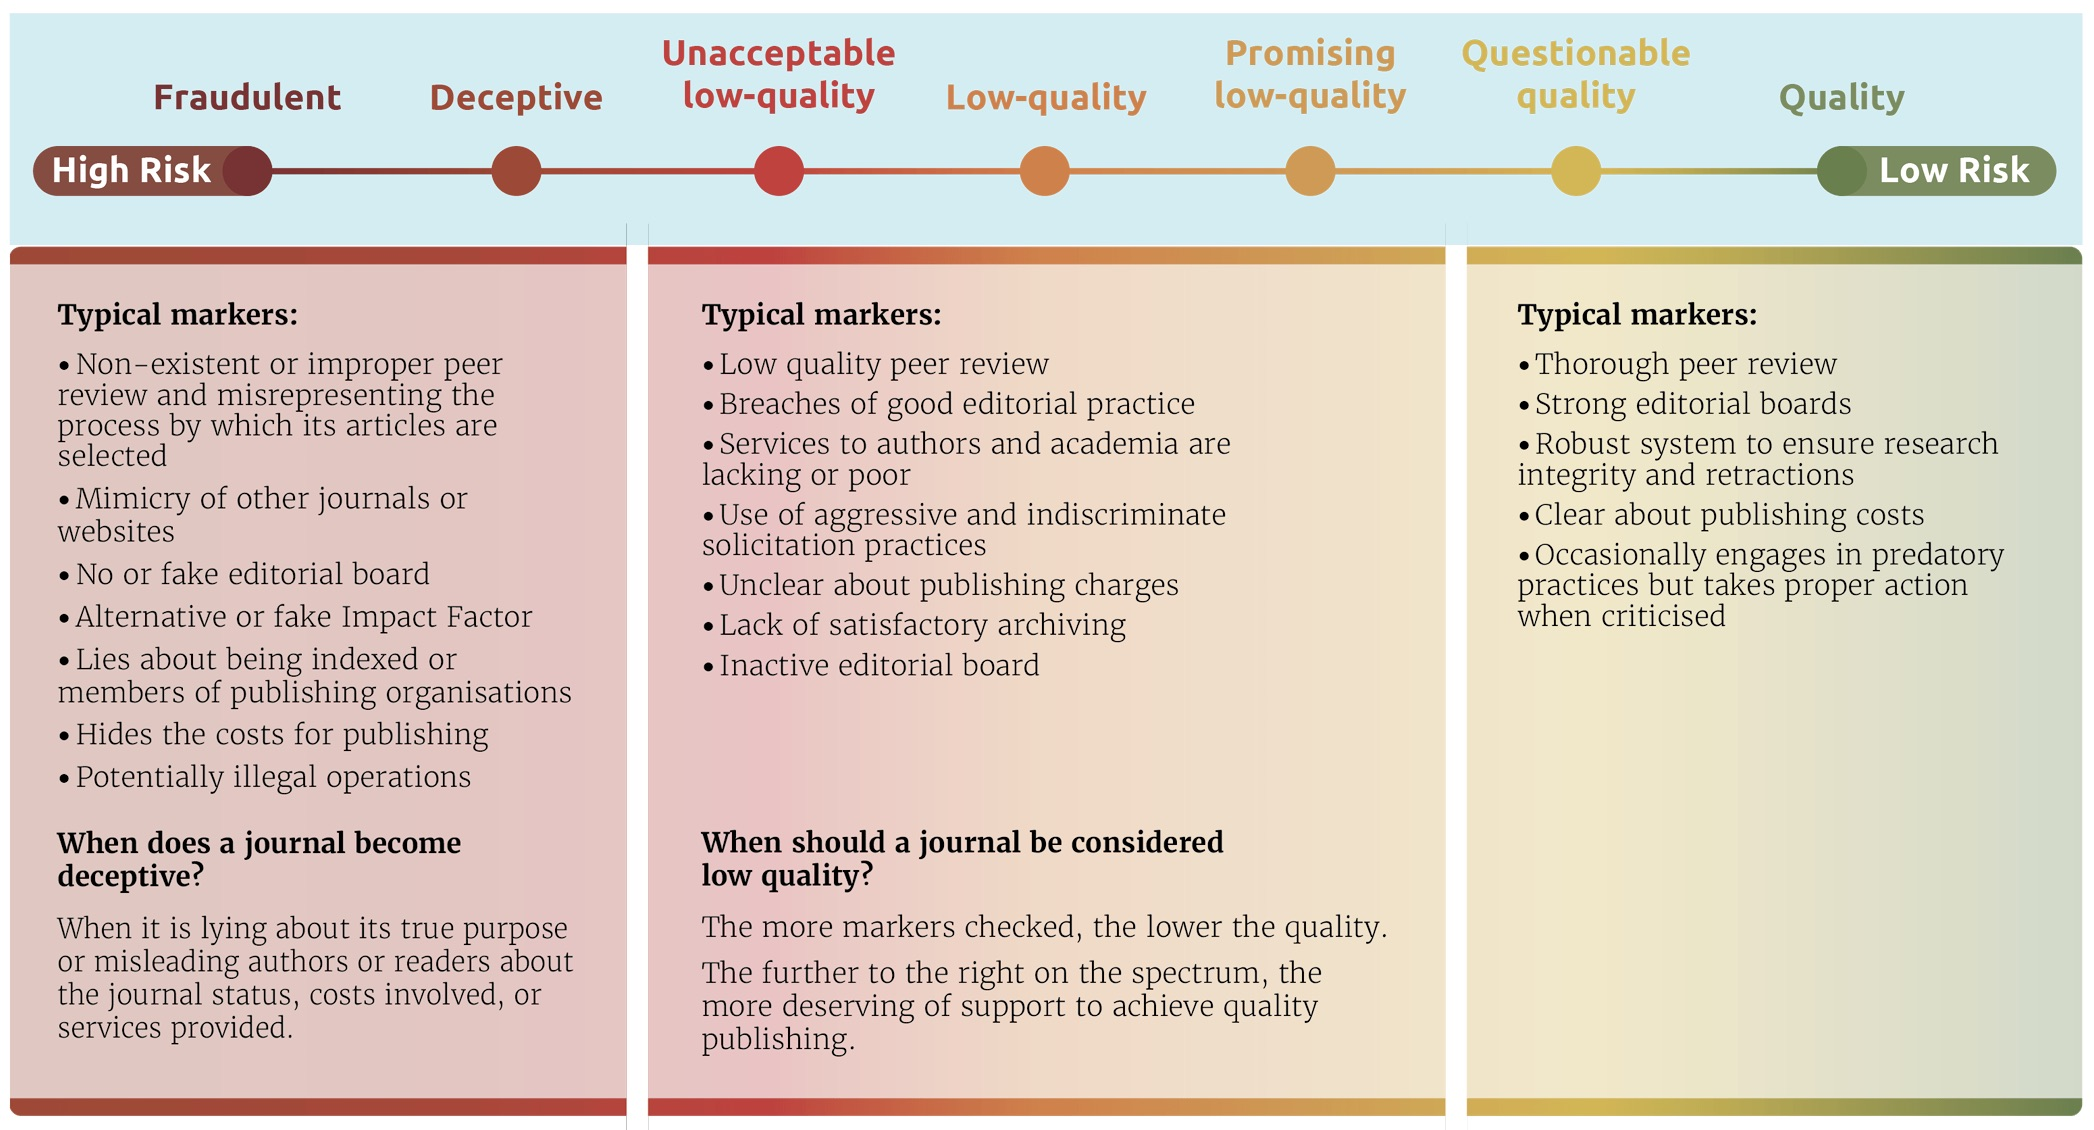
\includegraphics[width = \textwidth, height = 0.70\textheight]{Images/SpecJour.jpeg} \\
 {\color{blue}\href{https://www.interacademies.org/publication/predatory-practices-report-English}{Predatory Practice Report}}, InterAcademy Partnership (IAP)
\end{frame}
%%%%%%%%%%%

\begin{comment}
%%%%%%%%%%%
\begin{frame}{Identifying: Predatory Conferences Spectrum}
	\centering 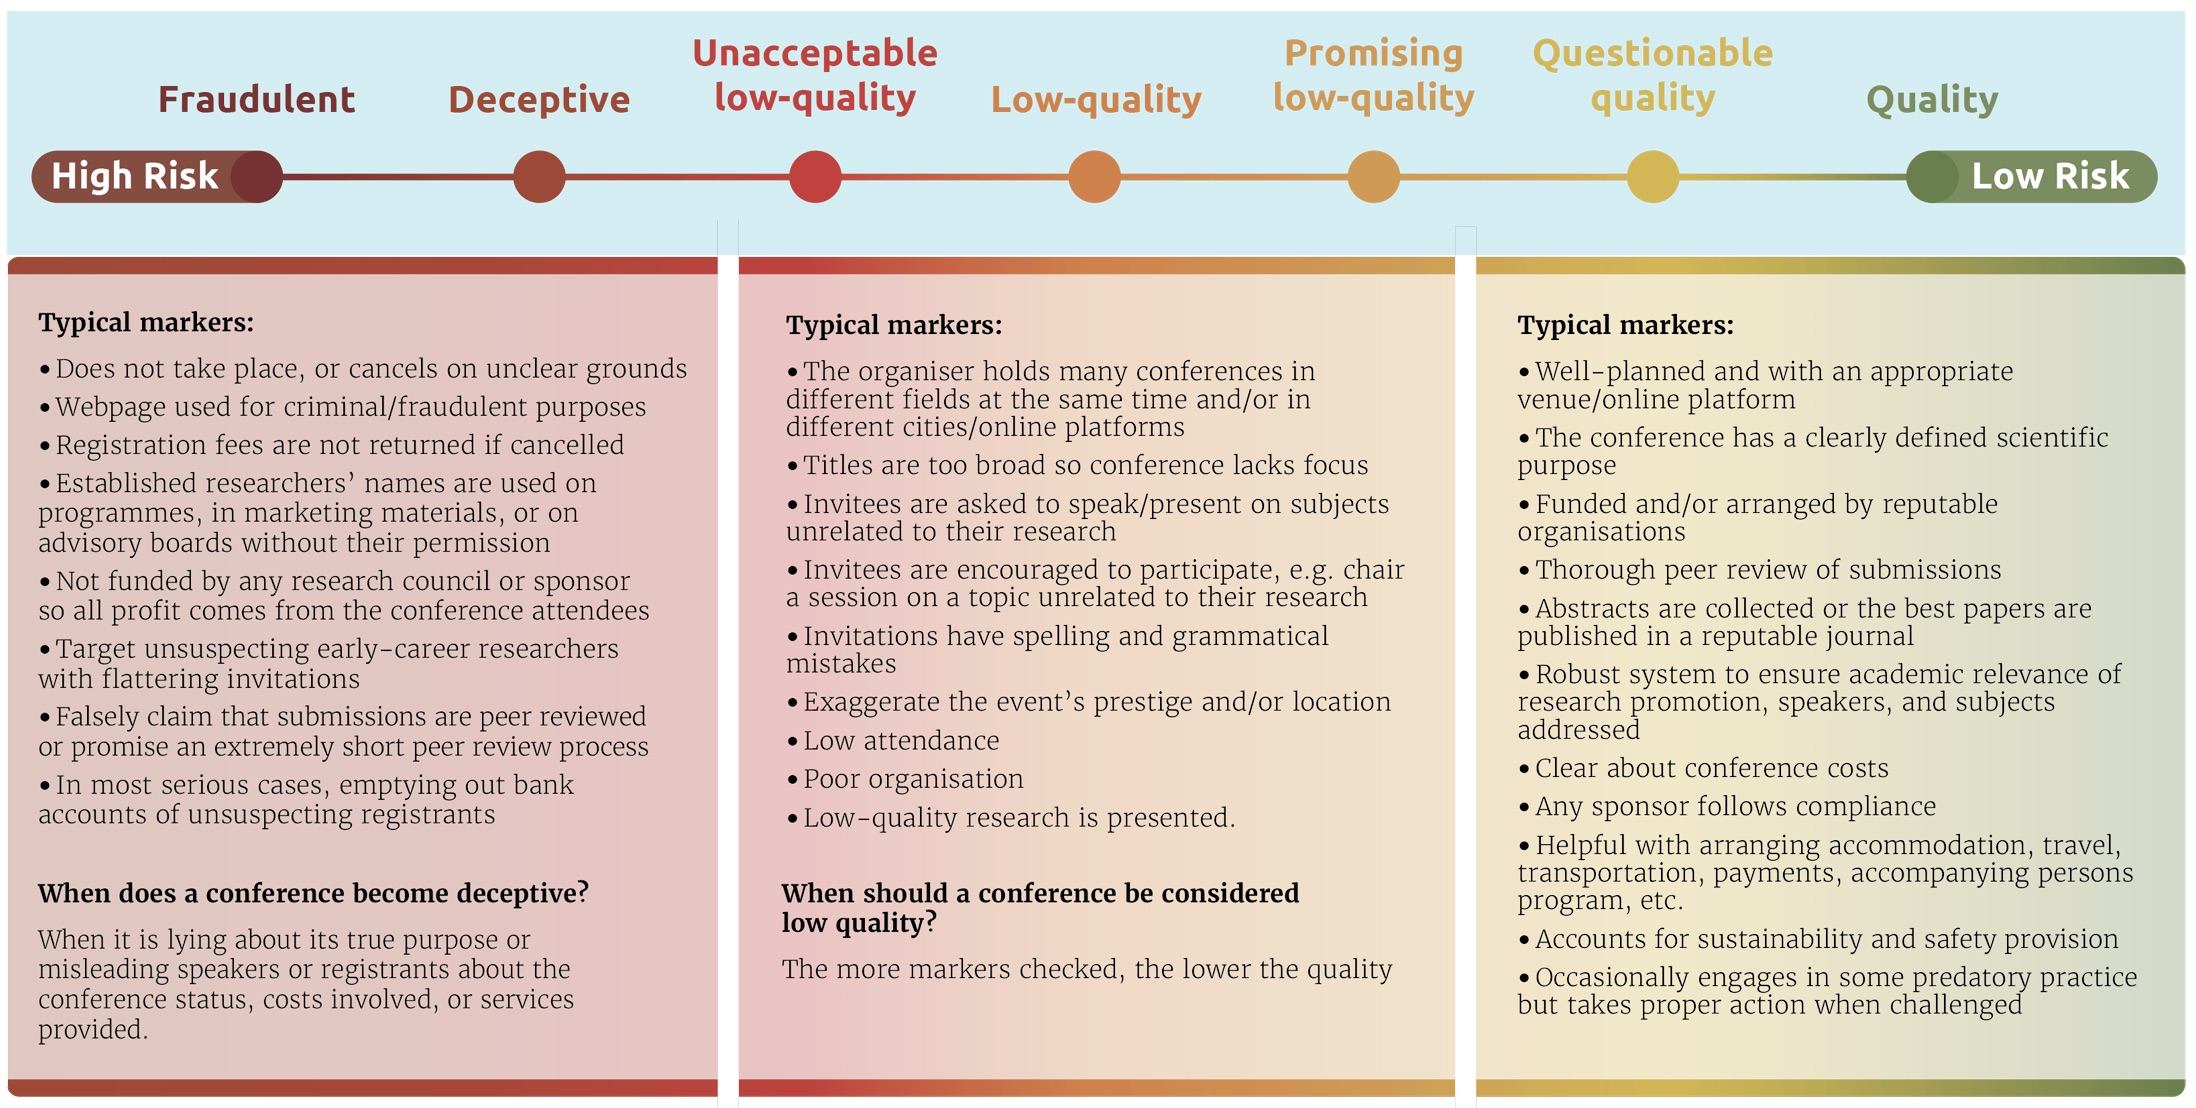
\includegraphics[width = \textwidth, height = 0.70\textheight]{Images/SpecConf.jpeg} \\
 {\color{blue}\href{https://www.interacademies.org/publication/predatory-practices-report-English}{Predatory Practice Report}}, IAP
\end{frame}
%%%%%%%%%%%
\end{comment}

\section{Summary:}
\subsection{Resources:}
%%%%%%%%%%%
\begin{frame}{Interesting Papers about Predatory Publishing:}
\begin{itemize}

    \item {\color{blue}\href{https://www.nature.com/articles/495433a}{Butler, 2013}}. Investigating journals: The dark side of publishing, \textit{Nature, 495, 433–435.}

    \item {\color{blue}\href{https://www.ncbi.nlm.nih.gov/pmc/articles/PMC5493177/}{Beall, 2017}}. What I learned from predatory publishers,  \textit{Biochemia Medica}.

    \item {\color{blue}\href{https://www.nature.com/articles/d41586-019-03759-y}{Grudniewicz et al., 2019}}. Predatory journals: no definition, no defence, \textit{Nature} 576, 210-212

    \item {\color{blue}\href{https://doi.org/10.1016/j.heliyon.2022.e08999}{Torress, 2022.}} Editorial misconduct: the case of online predatory journals,  \textit{Heliyon}.

    \item {\color{blue}\href{https://direct.mit.edu/qss/article/4/1/44/114726/Are-papers-published-in-predatory-journals}{Taskin et al., 2023}}. Are papers published in predatory journals worthless? A geopolitical dimension revealed by content-based analysis of citations, \textit{Quantitative Science Studies}, 4(1), 44–67.
\end{itemize}
\end{frame}

%%%%%%%%%%%
\begin{frame}{Additional Resources:}
	\begin{itemize} 
	\item List of {\color{blue}\href{https://predatoryreports.org/the-list}{predatory journals and publishers}} by {\color{blue}\href{https://predatoryreports.org/home}{Predatory Reports}}.
    \item Wikipedia: {\color{blue}\href{https://en.wikipedia.org/wiki/Predatory_publishing}{Predatory publishing}}.
    \item {\color{blue}\href{https://beckerguides.wustl.edu/selectingjournal}{Selecting a journal for publication}} by Washington University in St. Louis.
    \item \$500 per paper: {\color{blue}\href{https://www.fastcompany.com/3041493/why-a-fake-article-cuckoo-for-cocoa-puffs-was-accepted-by-17-medical-journals}{Why A Fake Article Titled “Cuckoo for Cocoa Puffs?” Was Accepted By 17 Medical Journals}}
    \item {\color{blue}\href{https://www.scidev.net/global/practical-guides/target-journal-right-research-communicate-publish}{How to target a right journal?}}
    \item News about retracted papers: {\color{blue}\href{https://retractionwatch.com/}{Retraction Watch}}.
    \item {\color{blue}\href{https://bijeshmishra.com/career-development/}{Tips and tricks:}} Resources about academic reading, writing, teaching, and predatory journals.
	\end{itemize}
\end{frame}
%%%%%%%%%%%

%%%%%%%%%%%
\begin{comment}
\begin{frame}{Power of Credibility}
Some authors are well established and have earned credibility. \\
Some MDPI journals are not considered predatory. \\
\smallskip
	\centering
\includegraphics[width = 0.8\textwidth, height = 0.7\textheight]{Images/Zilber1.png}
\end{frame}
%%%%%%%%%%%

%%%%%%%%%%%
\begin{frame}{}
 Some authors are well established and have earned credibility. \\ 
 Some MDPI journals are not considered predatory. \\
 \smallskip
	\centering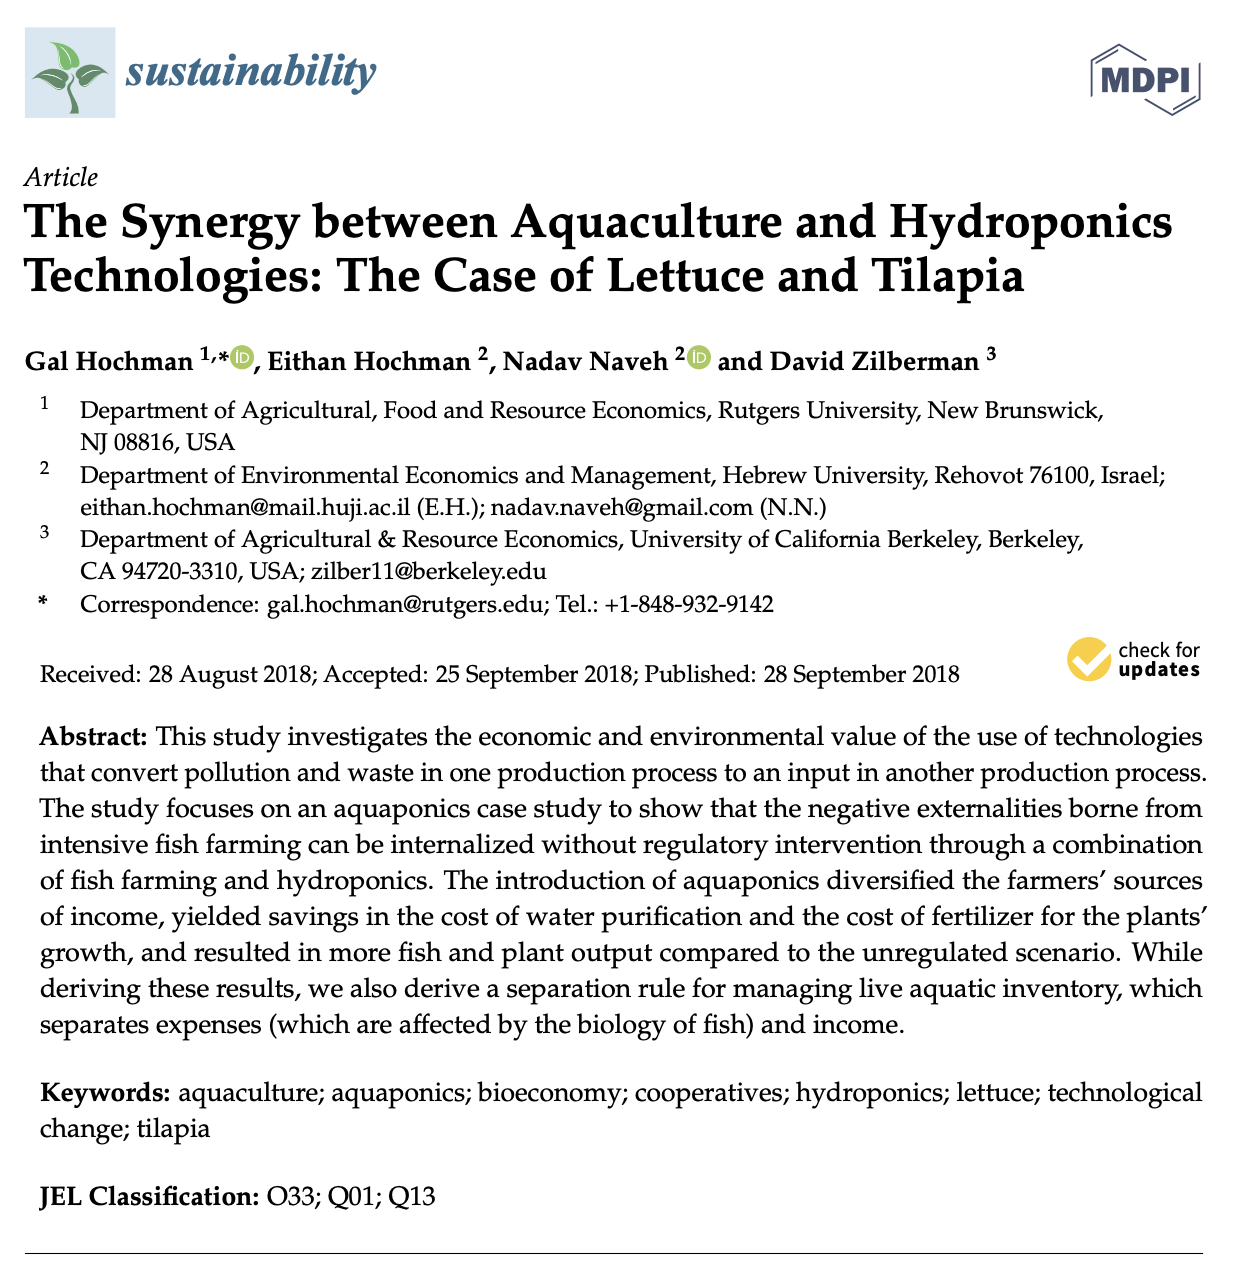
\includegraphics[width = 0.8\textwidth, height = 0.7\textheight]{Images/Zilber2.png} 
\end{frame}
\end{comment}
%%%%%%%%%%%

%%%%%%%%%%%
\begin{frame}{Learned Something or More Confused!?}
	\begin{itemize}
	\item Be self aware and seek help with peers.
	\item Judge based on transparency in publication process.
    \item Almost never pay to publish (fee $\approx$ {\color{red}\textbf{RED}} flag!).
    \item Research authenticity of publisher, editors, journals, and published papers before submitting paper.
	\item Do not hurry to publish: {\color{brown}\textbf{Quality research takes time!}}
    \item \textquotedblleft \textbf{Don't invite me, I'll reach to you!}\textquotedblright for publishing.
    \item \textbf{Final note:} Some papers published in predatory journals may be high quality but just unfortunate!
	\end{itemize}
\end{frame}
%%%%%%%%%%%

\section{Reading Paper}
%%%%%%%%%%%%%%%%%%
\subsection{Reading Paper}
\begin{frame}{Part II: Reading Peer-reviewed Journal Article}
    \textbf{Parts of Scientific Paper} (General Structure)
        \vspace{0.3cm}
        \begin{itemize}
            \item Abstract
            \vspace{0.1cm}
            \item Introduction
                \begin{itemize}
                    \item Motivation
                    \item Purpose (objective) of research
                    \item Research gap
                    \item Work done
                    \item Novelty
                    \item Summary of findings
                \end{itemize}
                \vspace{0.1cm}
            \item Method and Materials
                \begin{itemize}
                    \item Study area
                    \item Data collection
                    \item Data analysis
                \end{itemize}
        \end{itemize}
\end{frame}

\begin{frame}{Reading Peer-reviewed Journal Article}
\textbf{Parts of Scientific Paper} (General Structure) (Cont...)
\vspace{0.3cm}
\begin{itemize}
    \item Result and discussion
        \begin{itemize}
            \item Findings in detail
            \item Support or contrast findings in relation to past research
        \end{itemize}
        \vspace{0.1cm}
    \item Conclusion
        \begin{itemize}
            \item Overall relationship with the objective of research
            \item Policy implications
            \item limitations of research
            \item anything else directly related to research 
            \item {\color{red}CAUTION:} Not an information dumping site
        \end{itemize}
\end{itemize}
Three examples in next few slides: {\color{blue}\href{https://doi.org/10.1016/j.jenvman.2023.118225}{Mishra et al., 2023}}, {\color{blue}\href{https://doi.org/10.1016/j.foreco.2023.120987}{McKinney et al., 2023}}, {\color{blue}\href{https://doi.org/10.1080/09603123.2019.1602252}{Antonious et al., 2019}}.
\end{frame}

\begin{frame}{}
    \centering 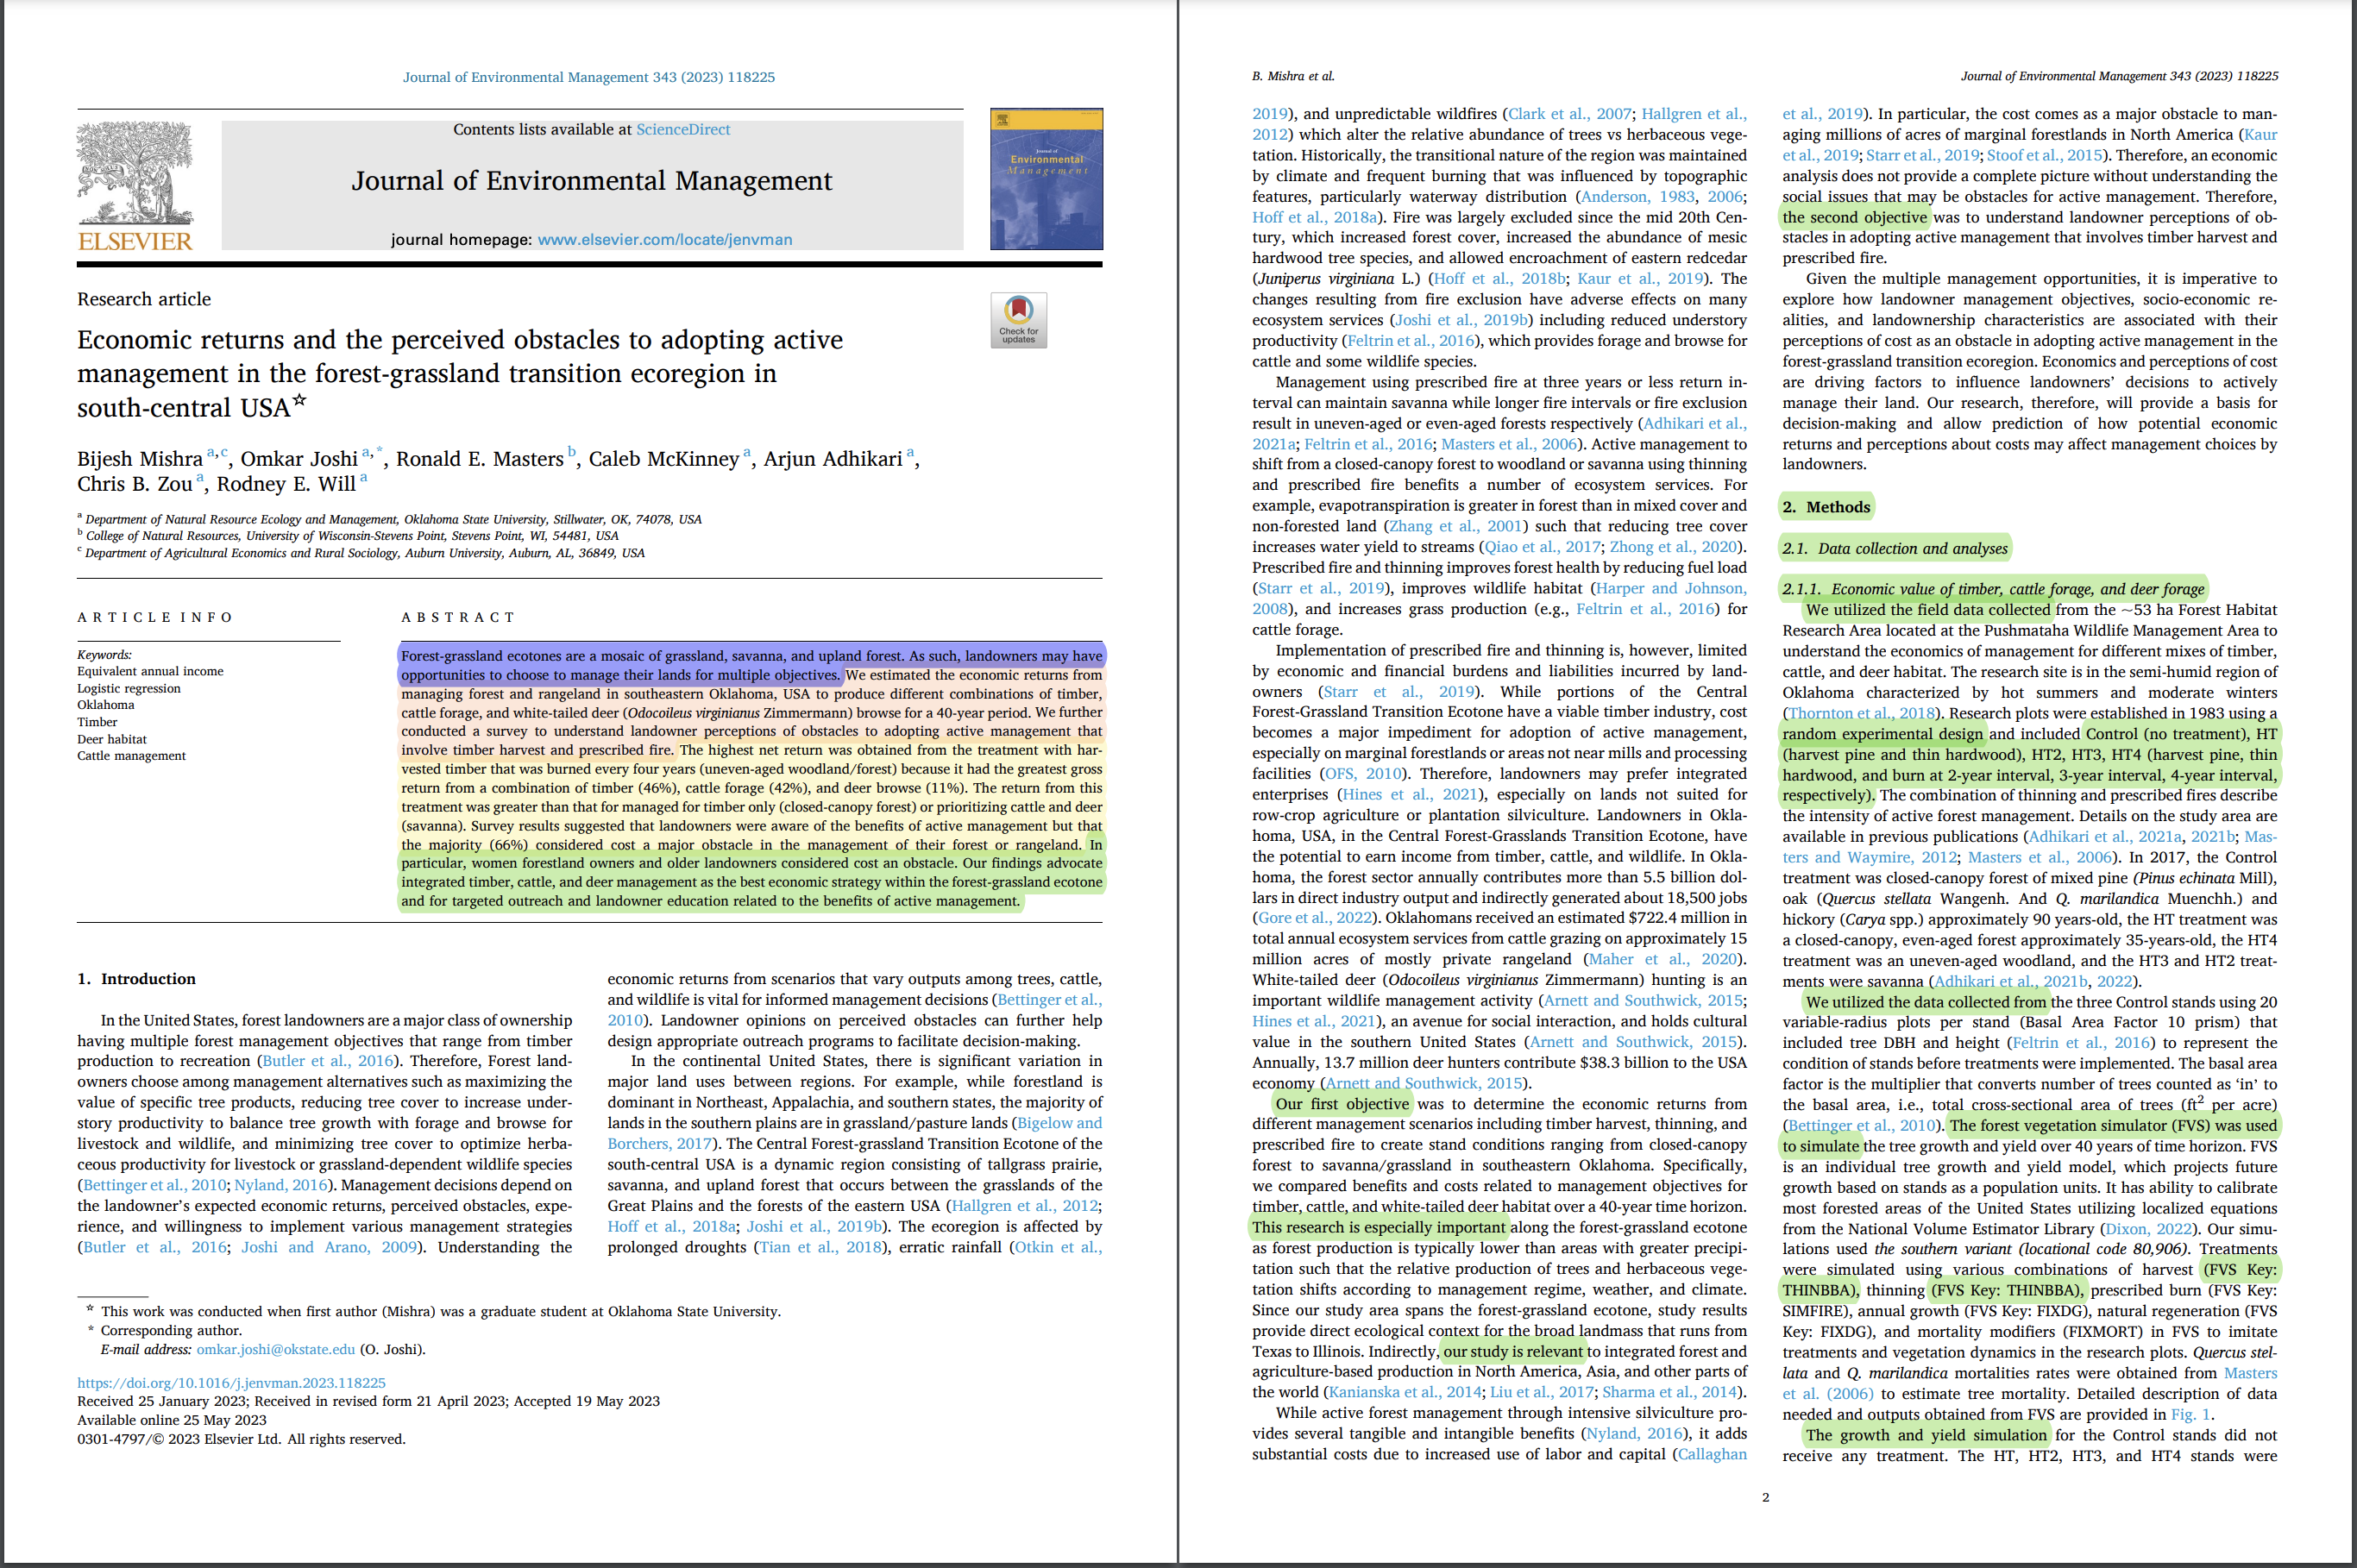
\includegraphics[width = \textwidth, height = 0.90\textheight]{Images/Jem1.png}
\end{frame}

\begin{frame}{}
    \centering 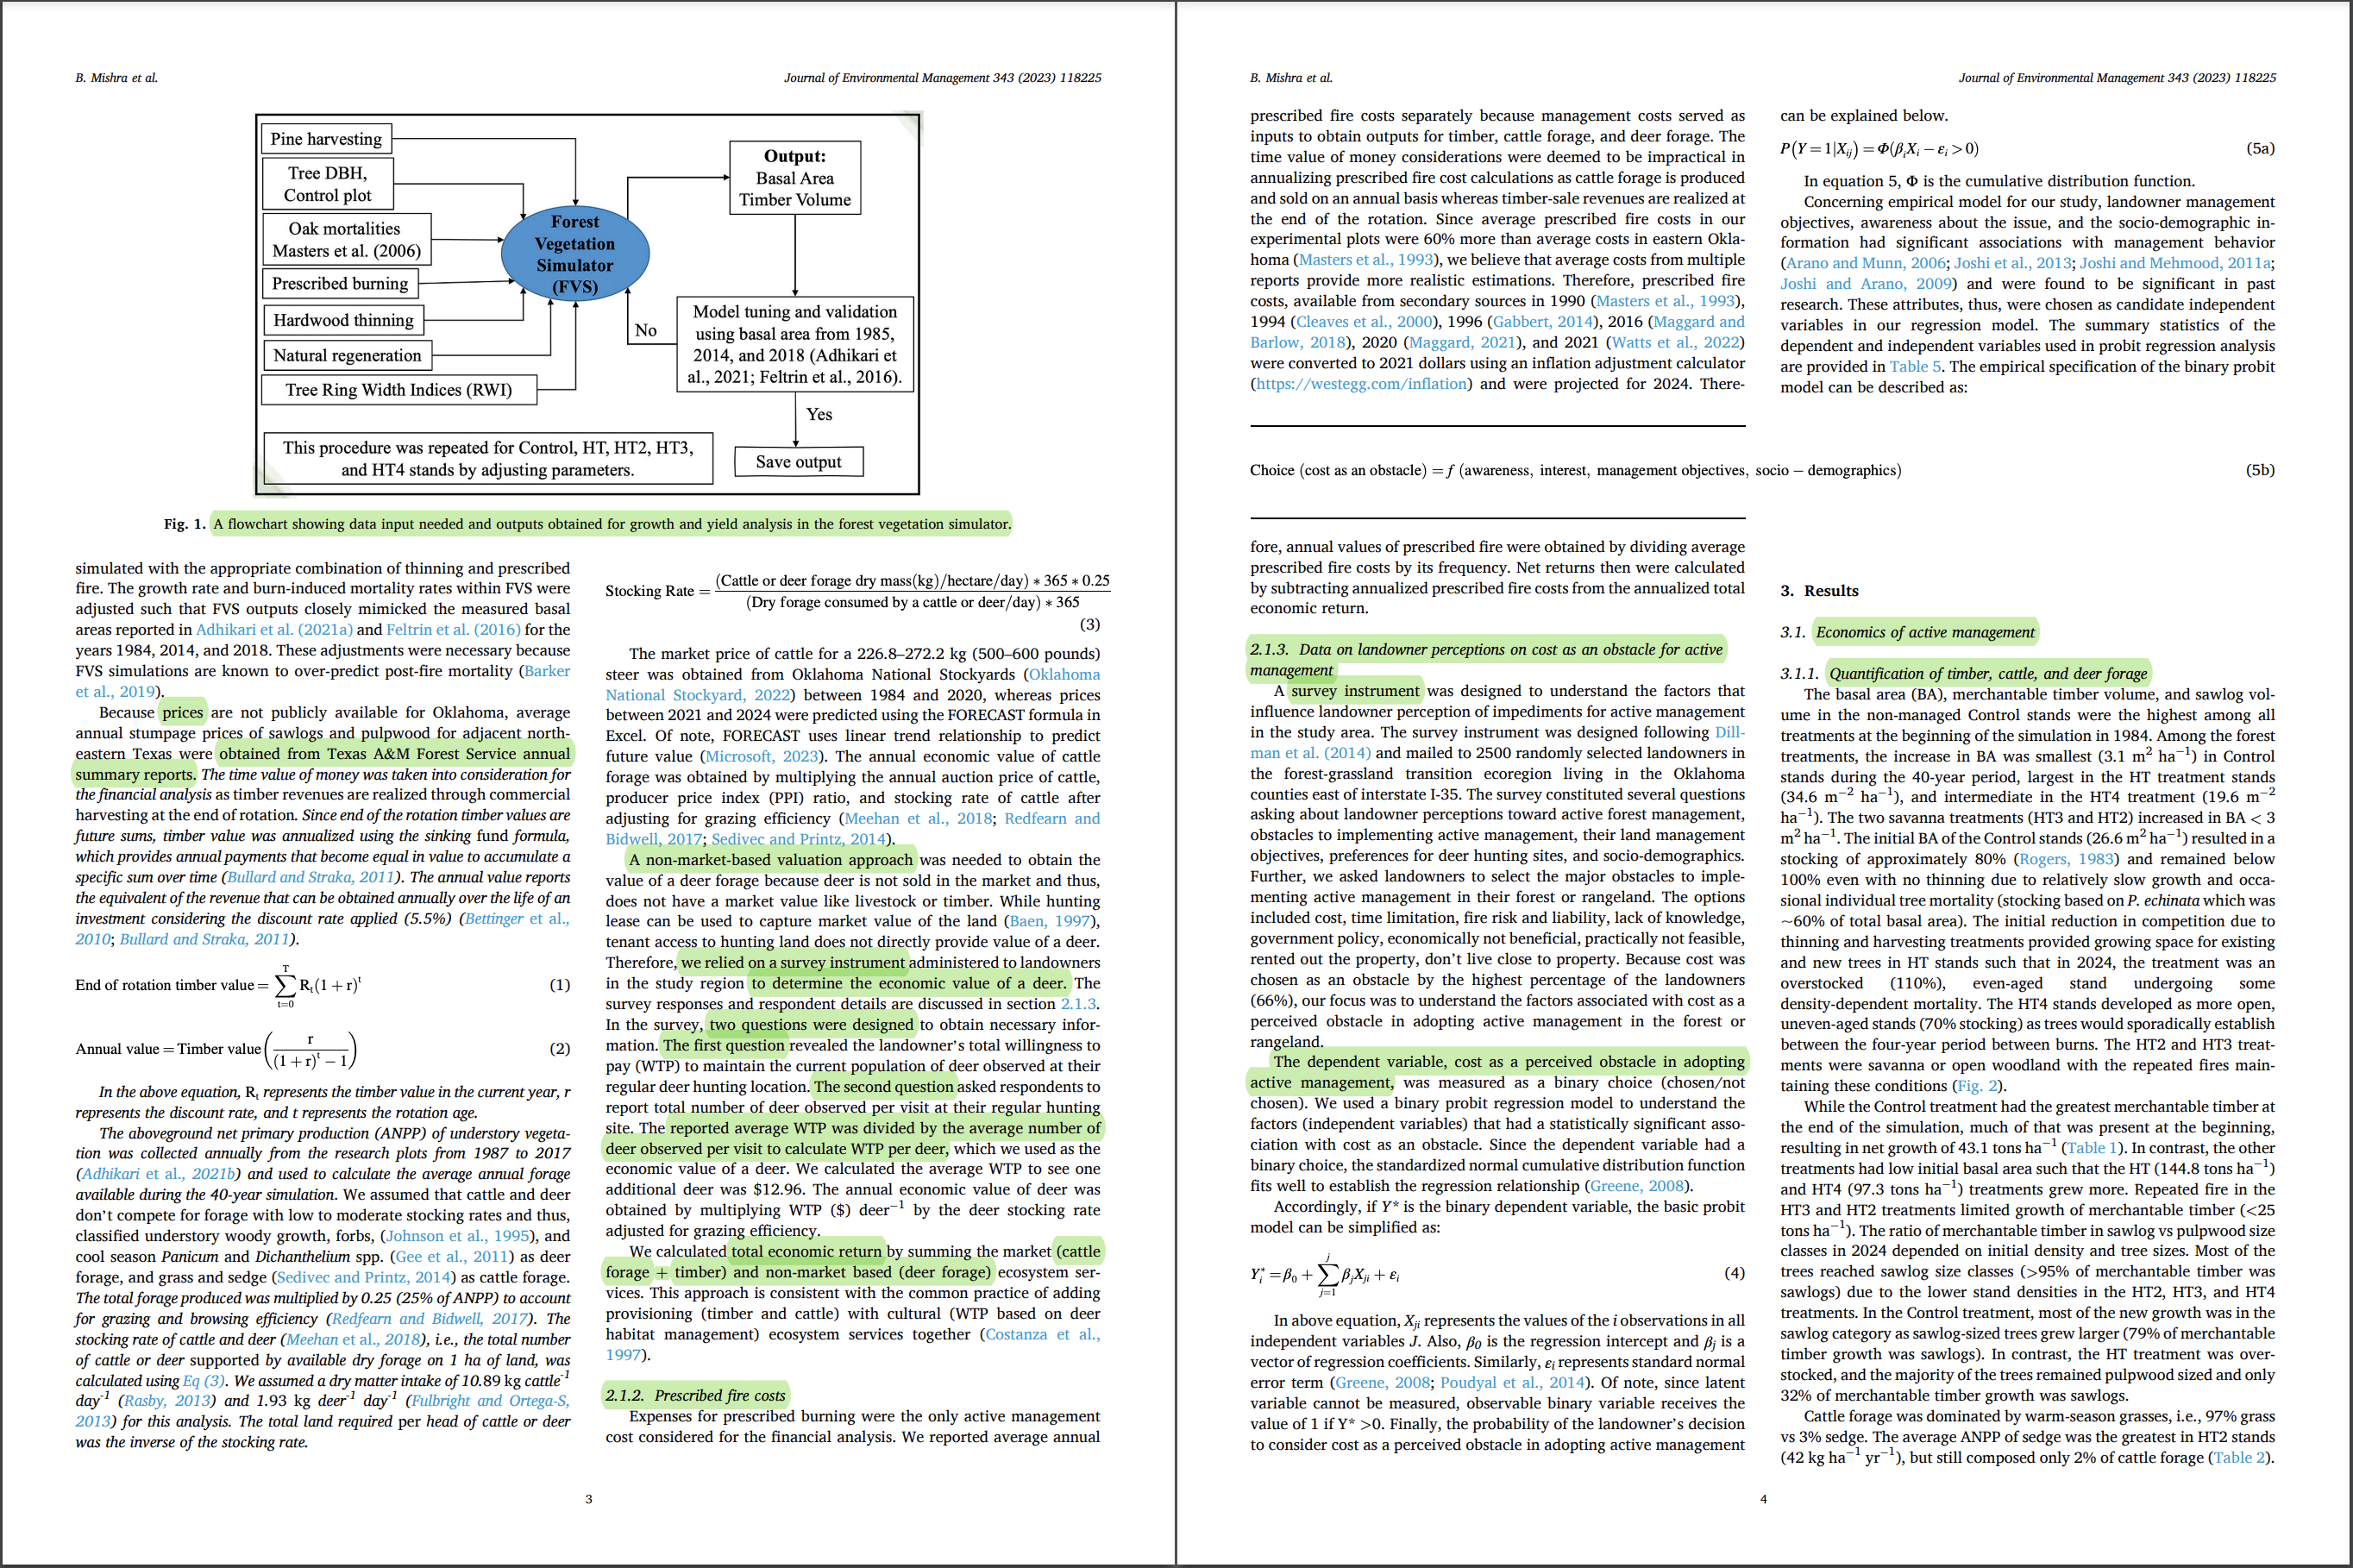
\includegraphics[width = \textwidth, height = 0.95\textheight]{Images/Jem2.png}
\end{frame}

\begin{frame}{}
    \centering 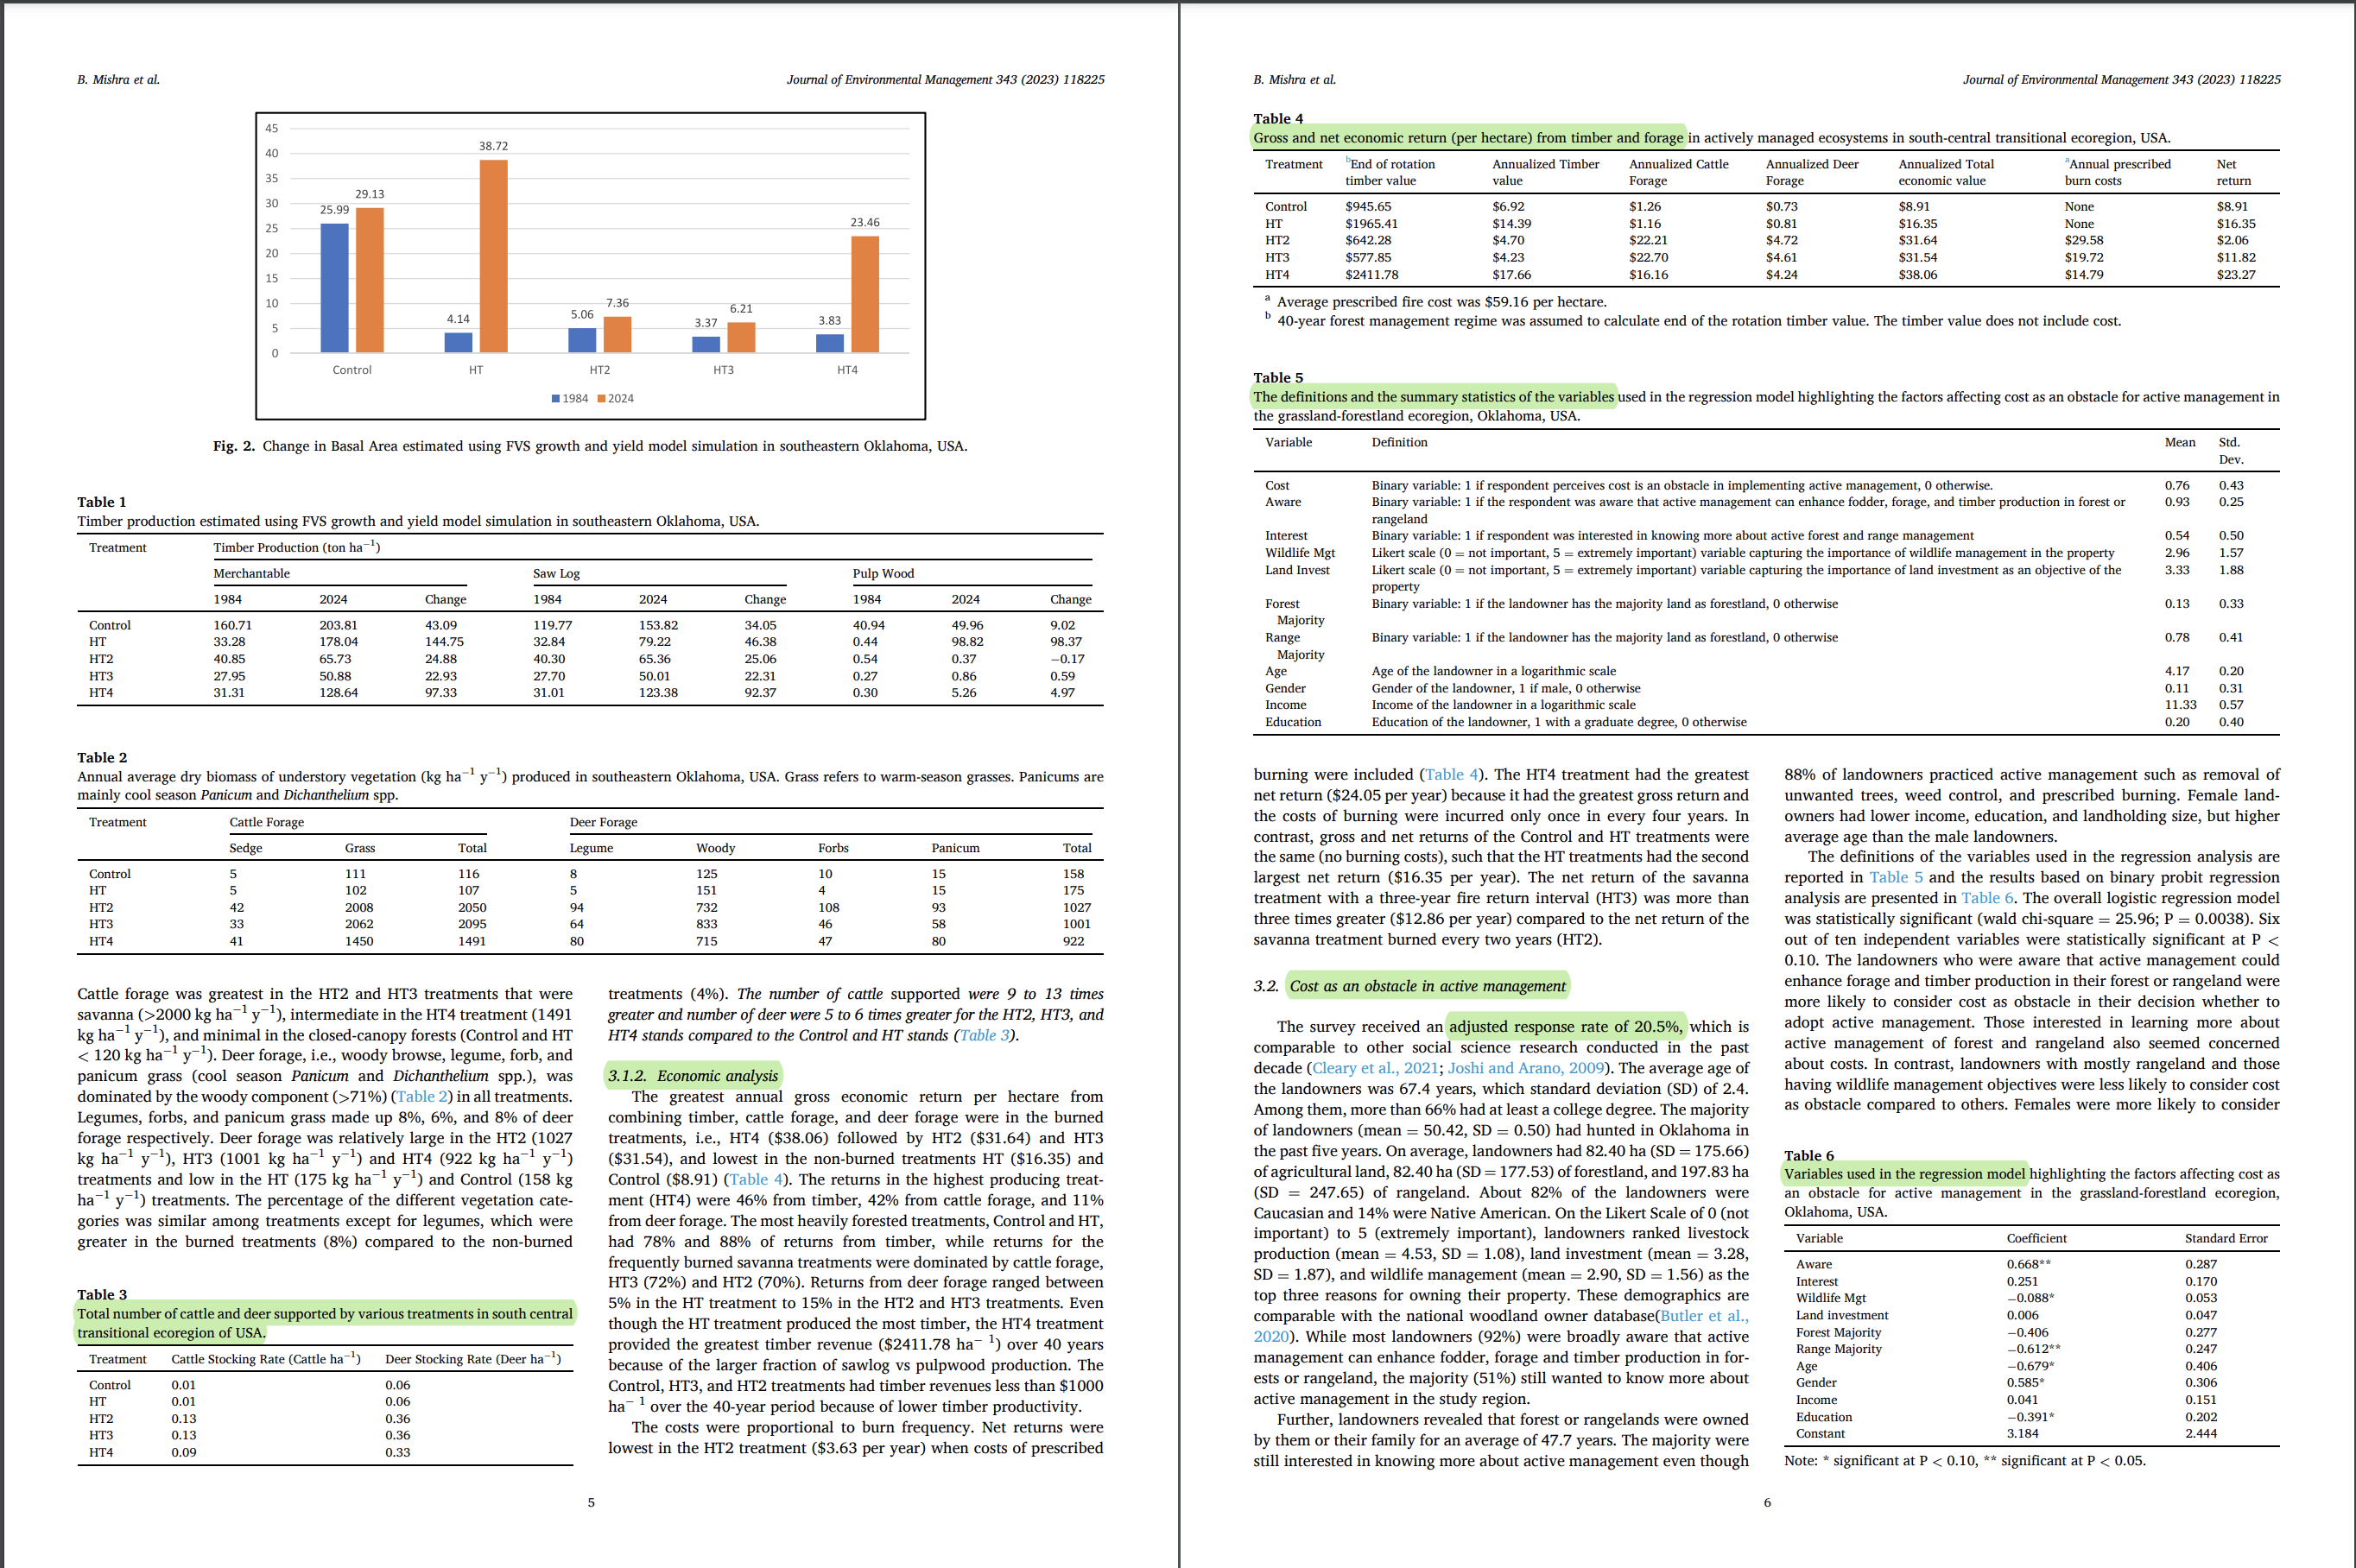
\includegraphics[width = \textwidth, height = 0.95\textheight]{Images/Jem3.png}
\end{frame}

\begin{frame}{}
    \centering 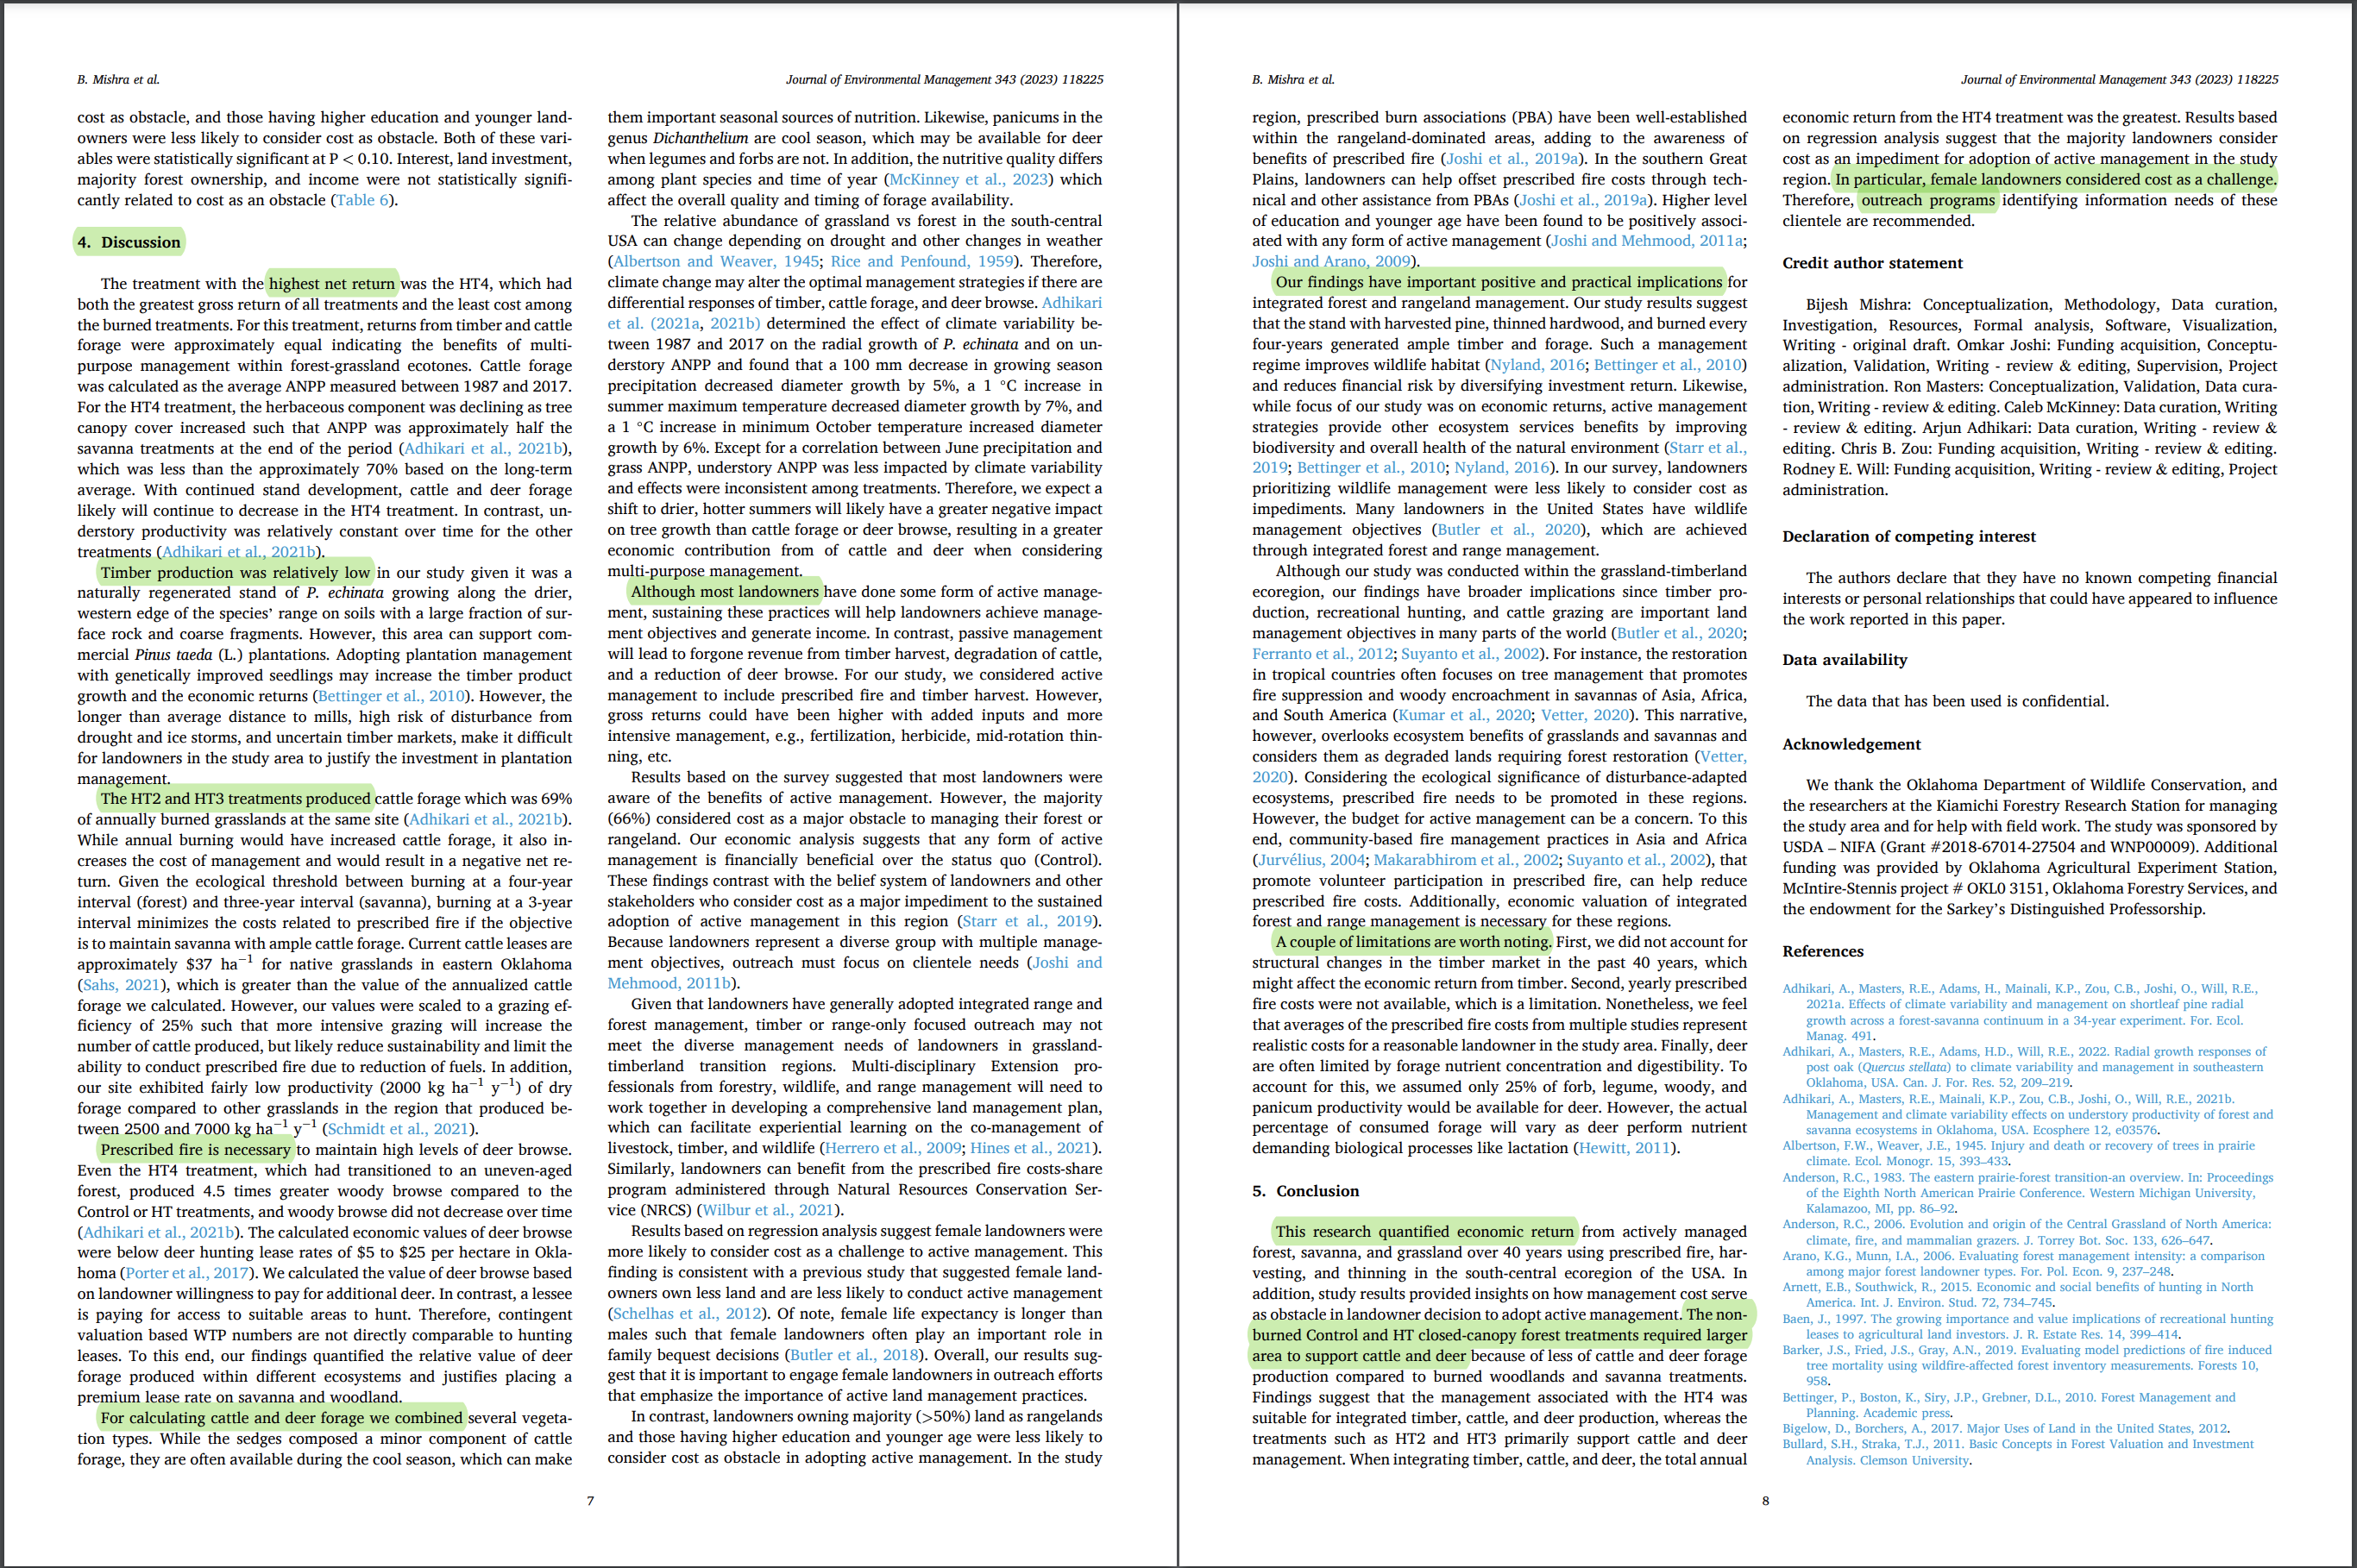
\includegraphics[width = \textwidth, height = 0.95\textheight]{Images/Jem4.png}
\end{frame}

\begin{frame}{}
    \centering 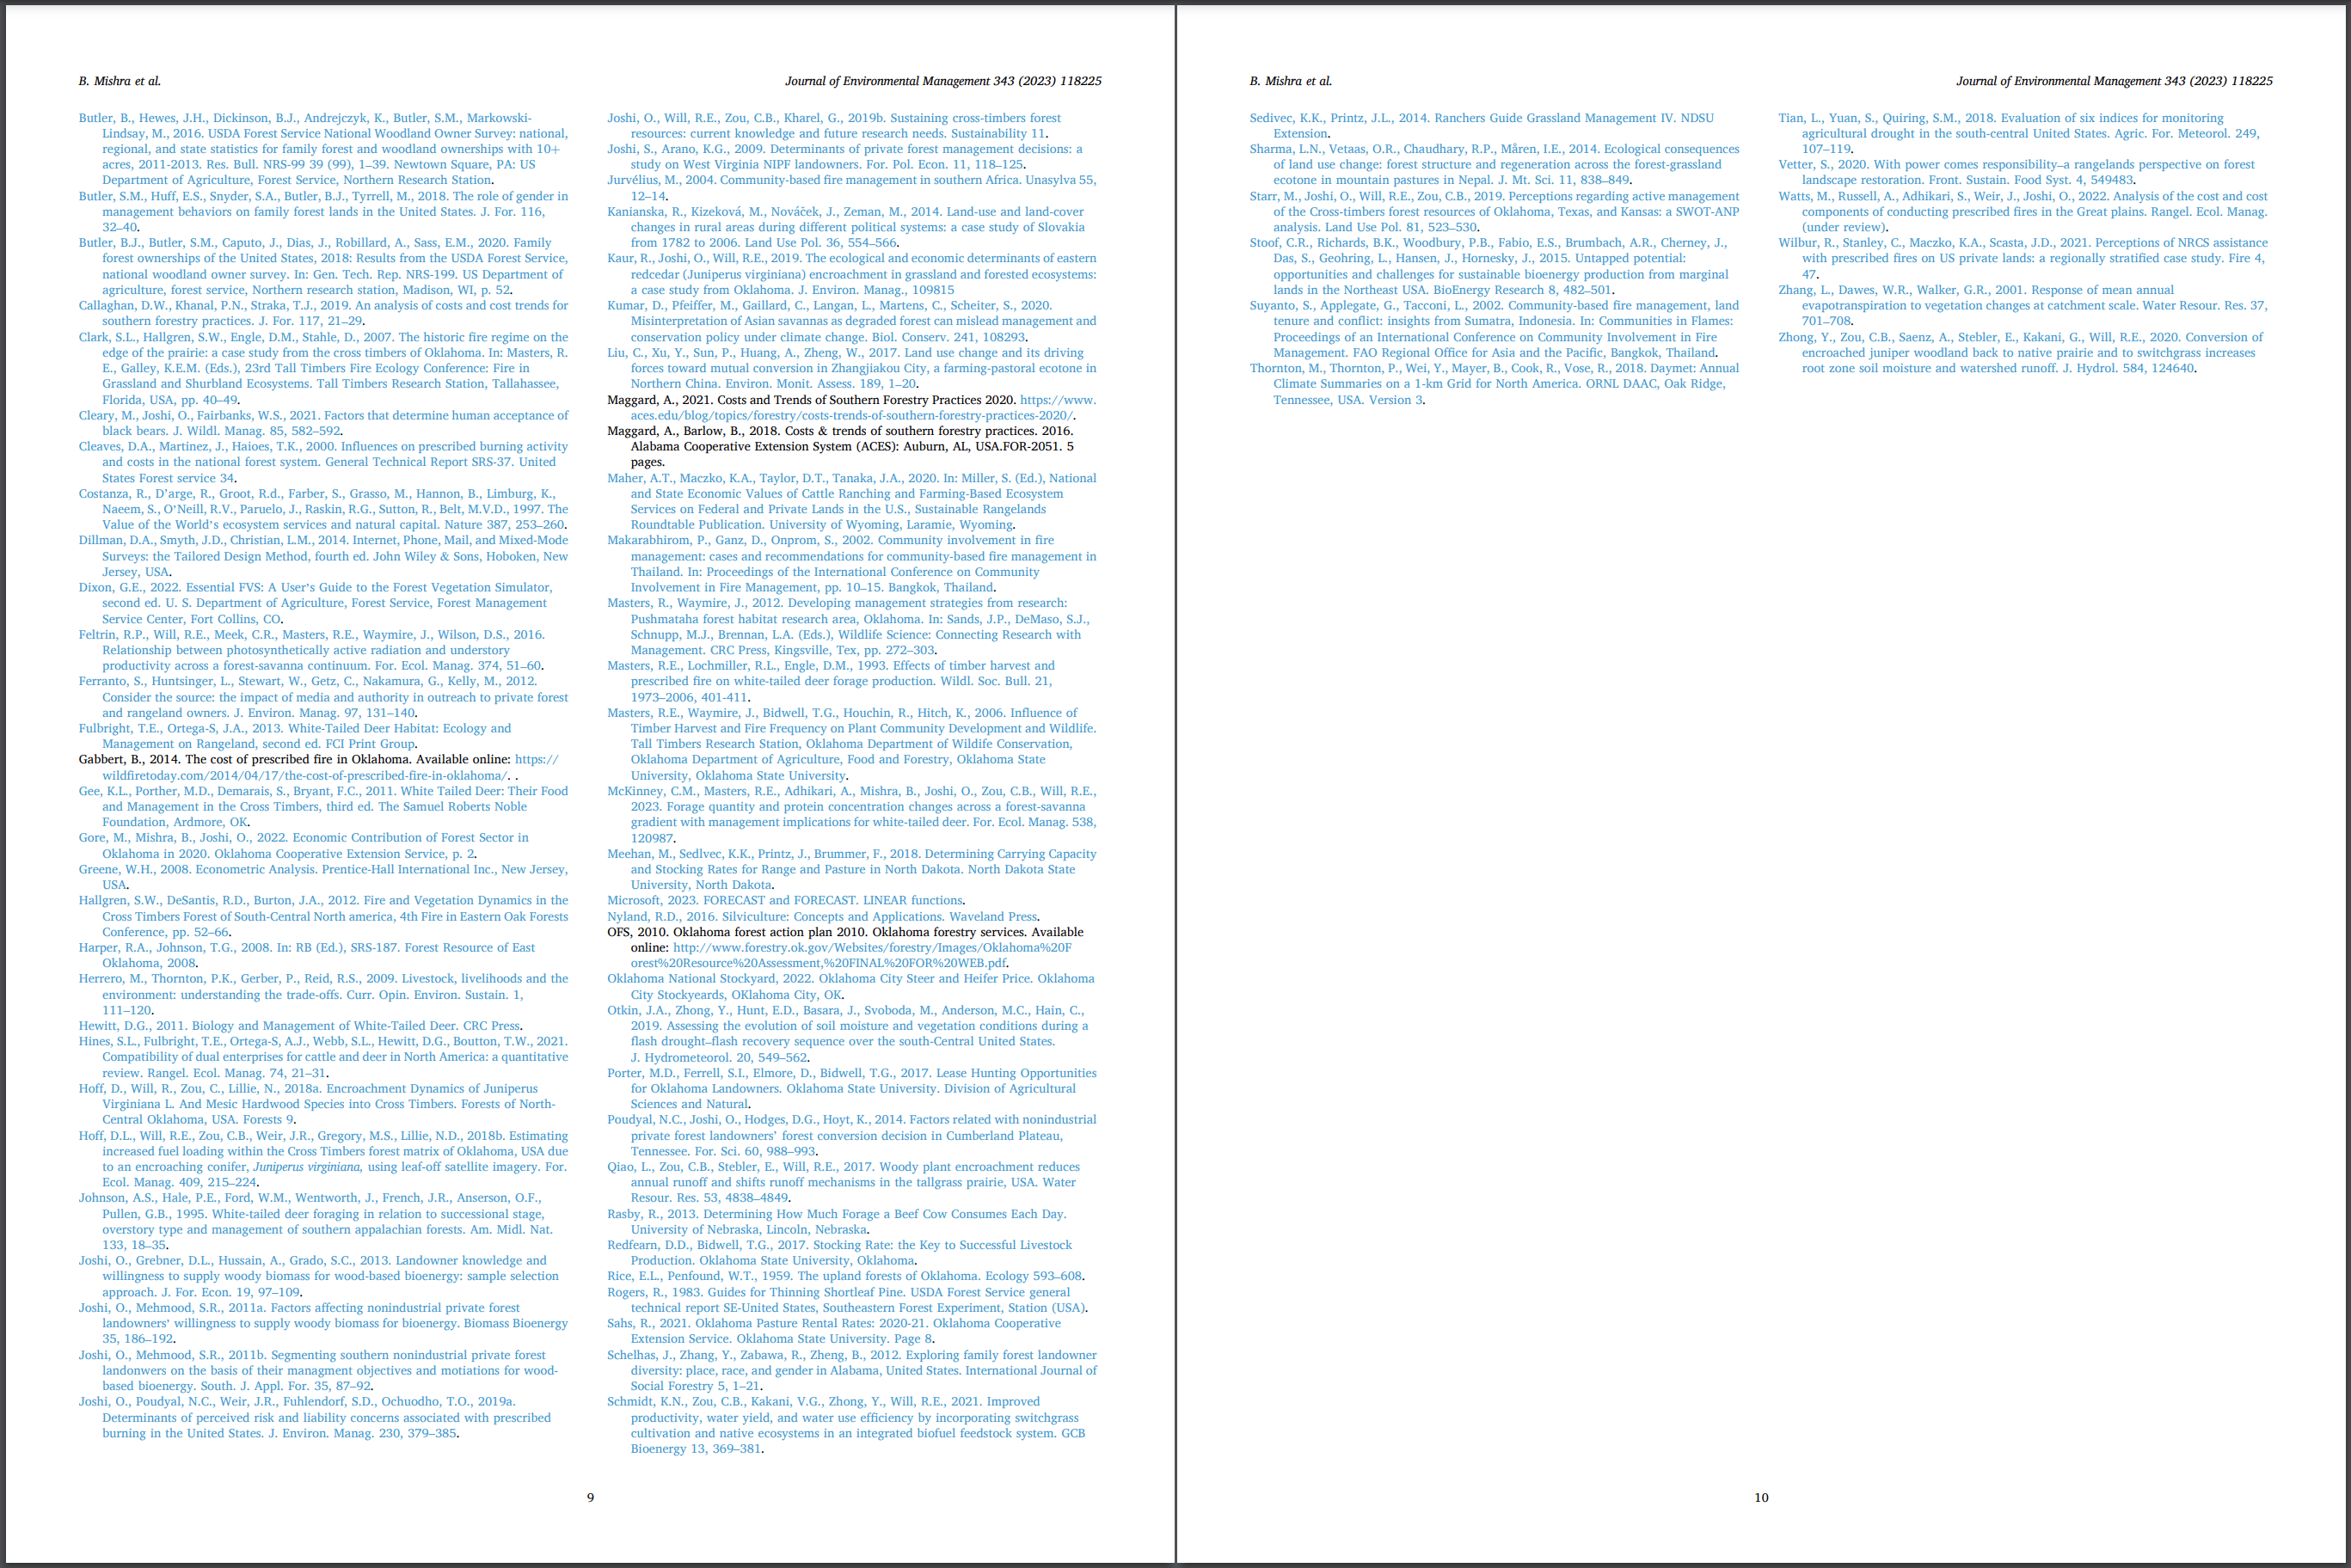
\includegraphics[width = \textwidth, height = 0.95\textheight]{Images/Jem5.png}
\end{frame}

\begin{frame}{}
    \centering 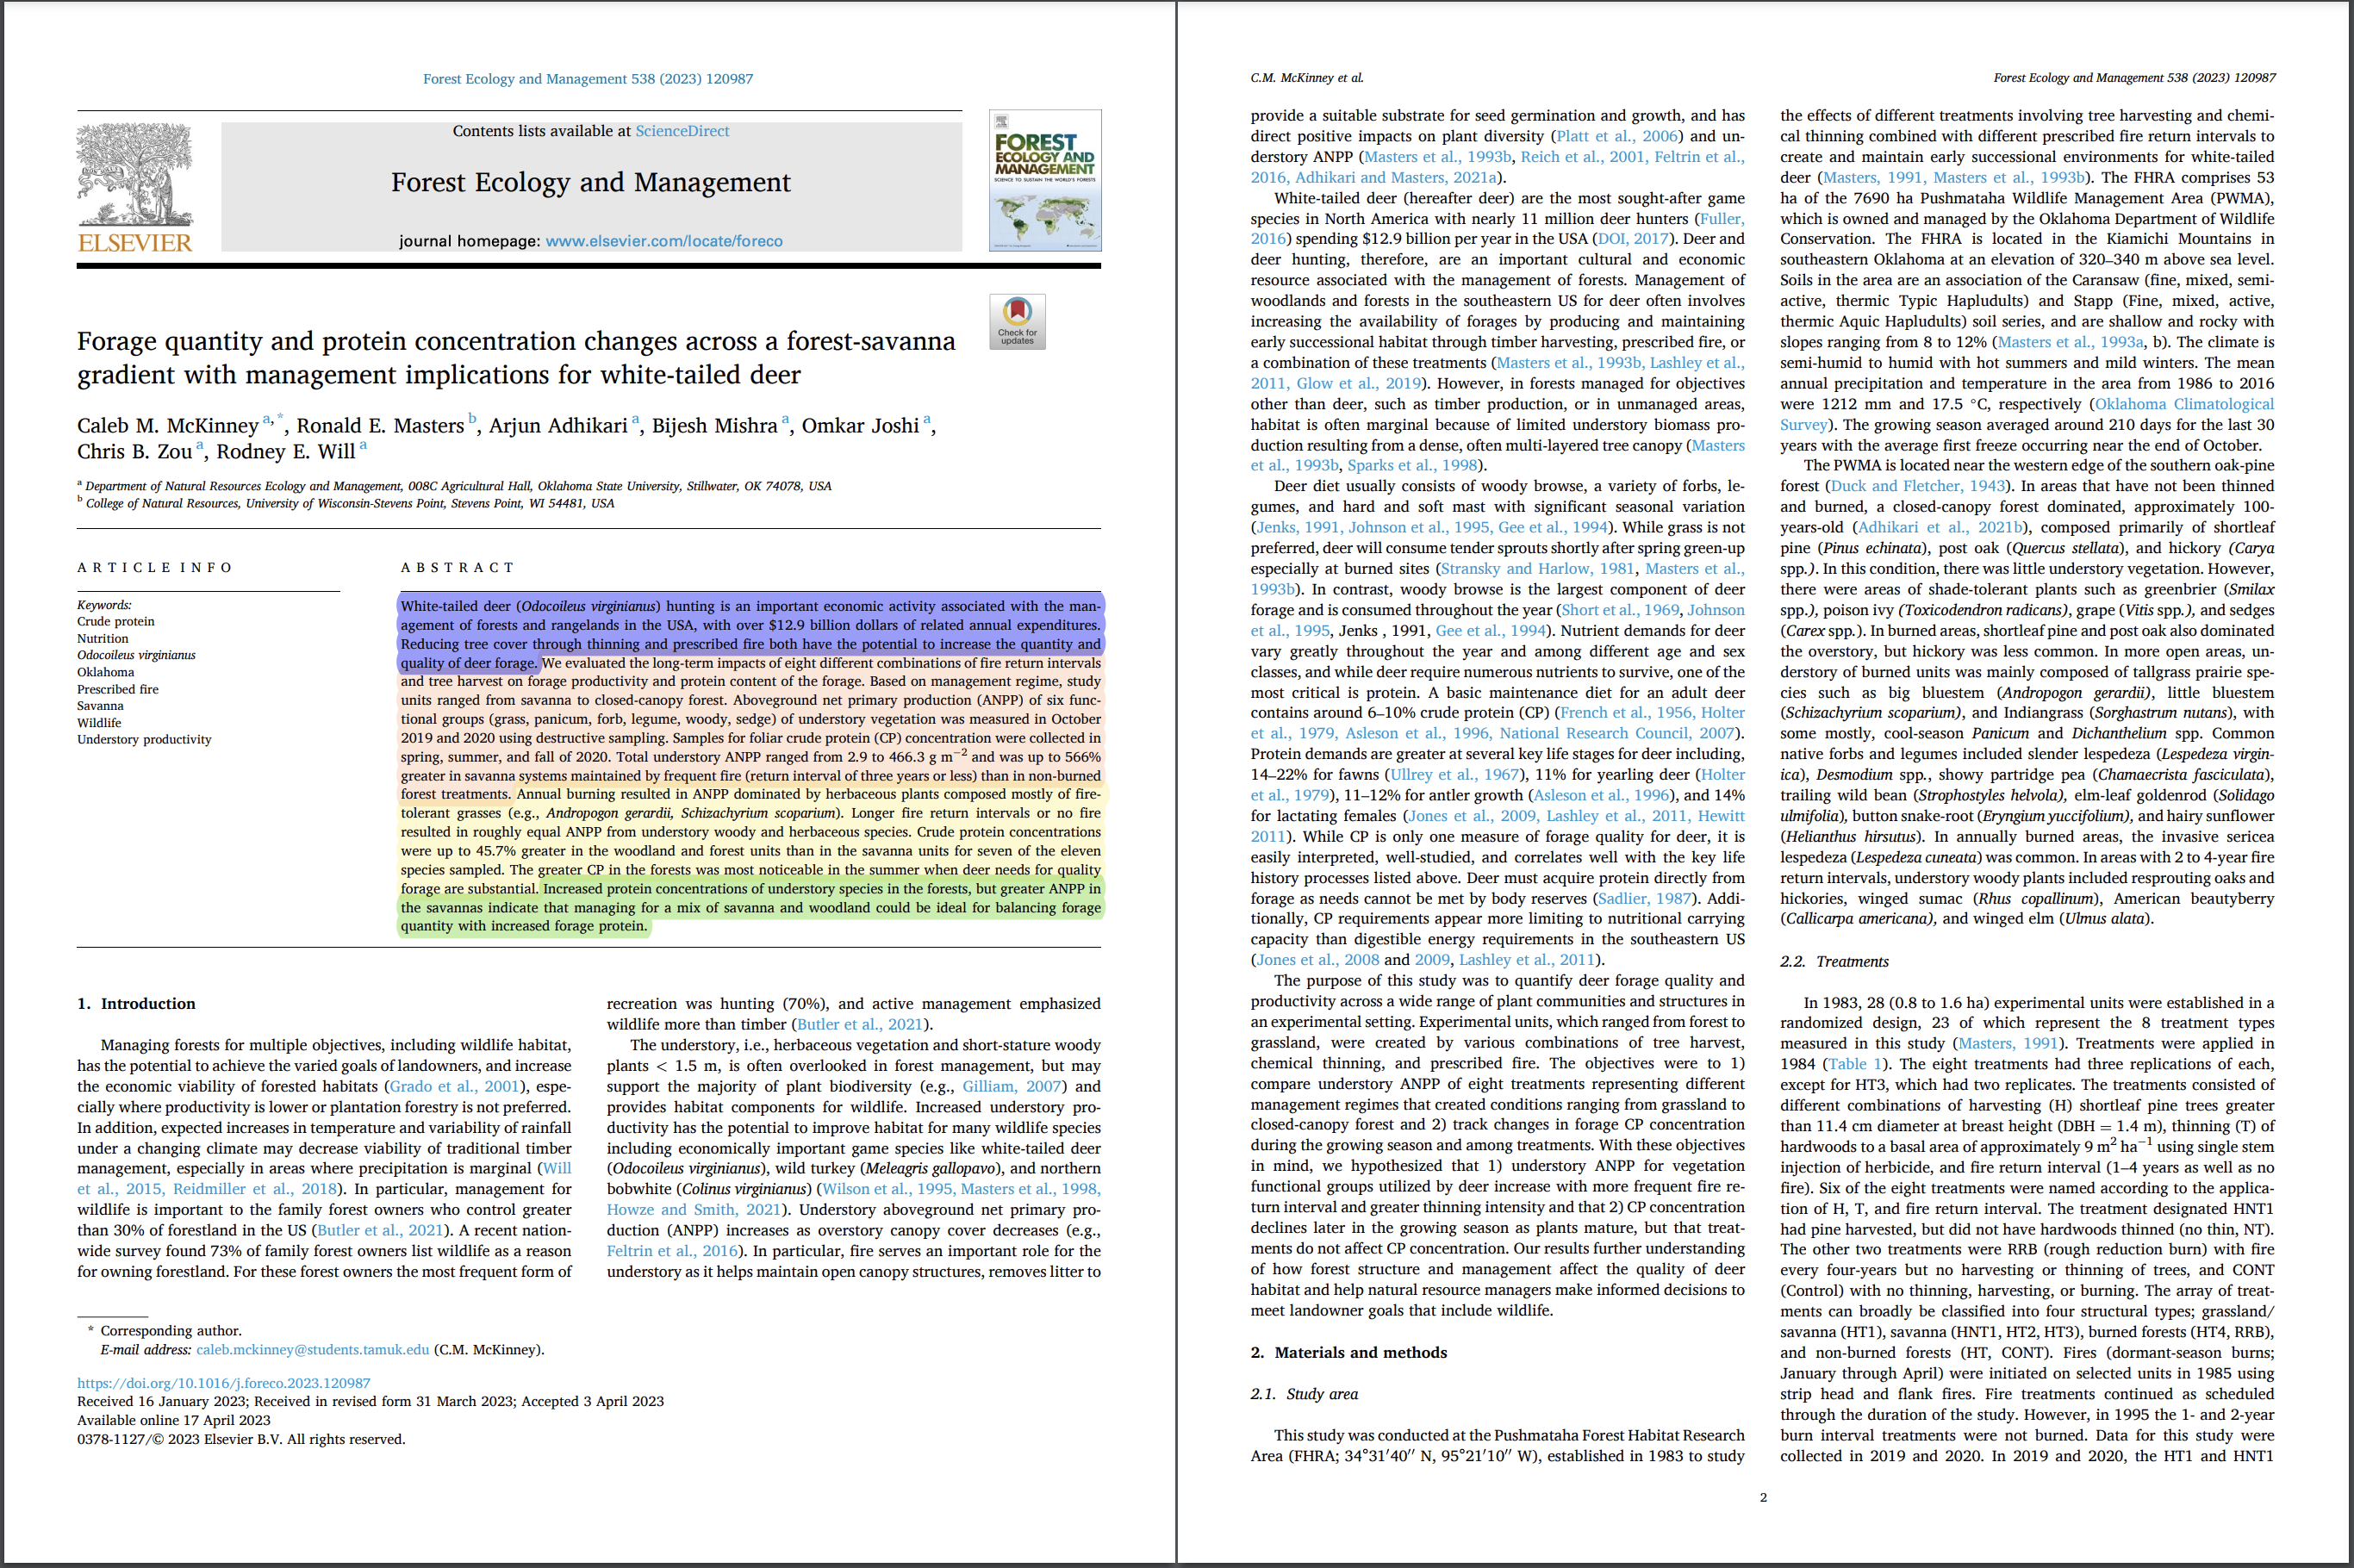
\includegraphics[width = \textwidth, height = 0.95\textheight]{Images/Forest1.png}
\end{frame}

\begin{frame}{}
    \centering 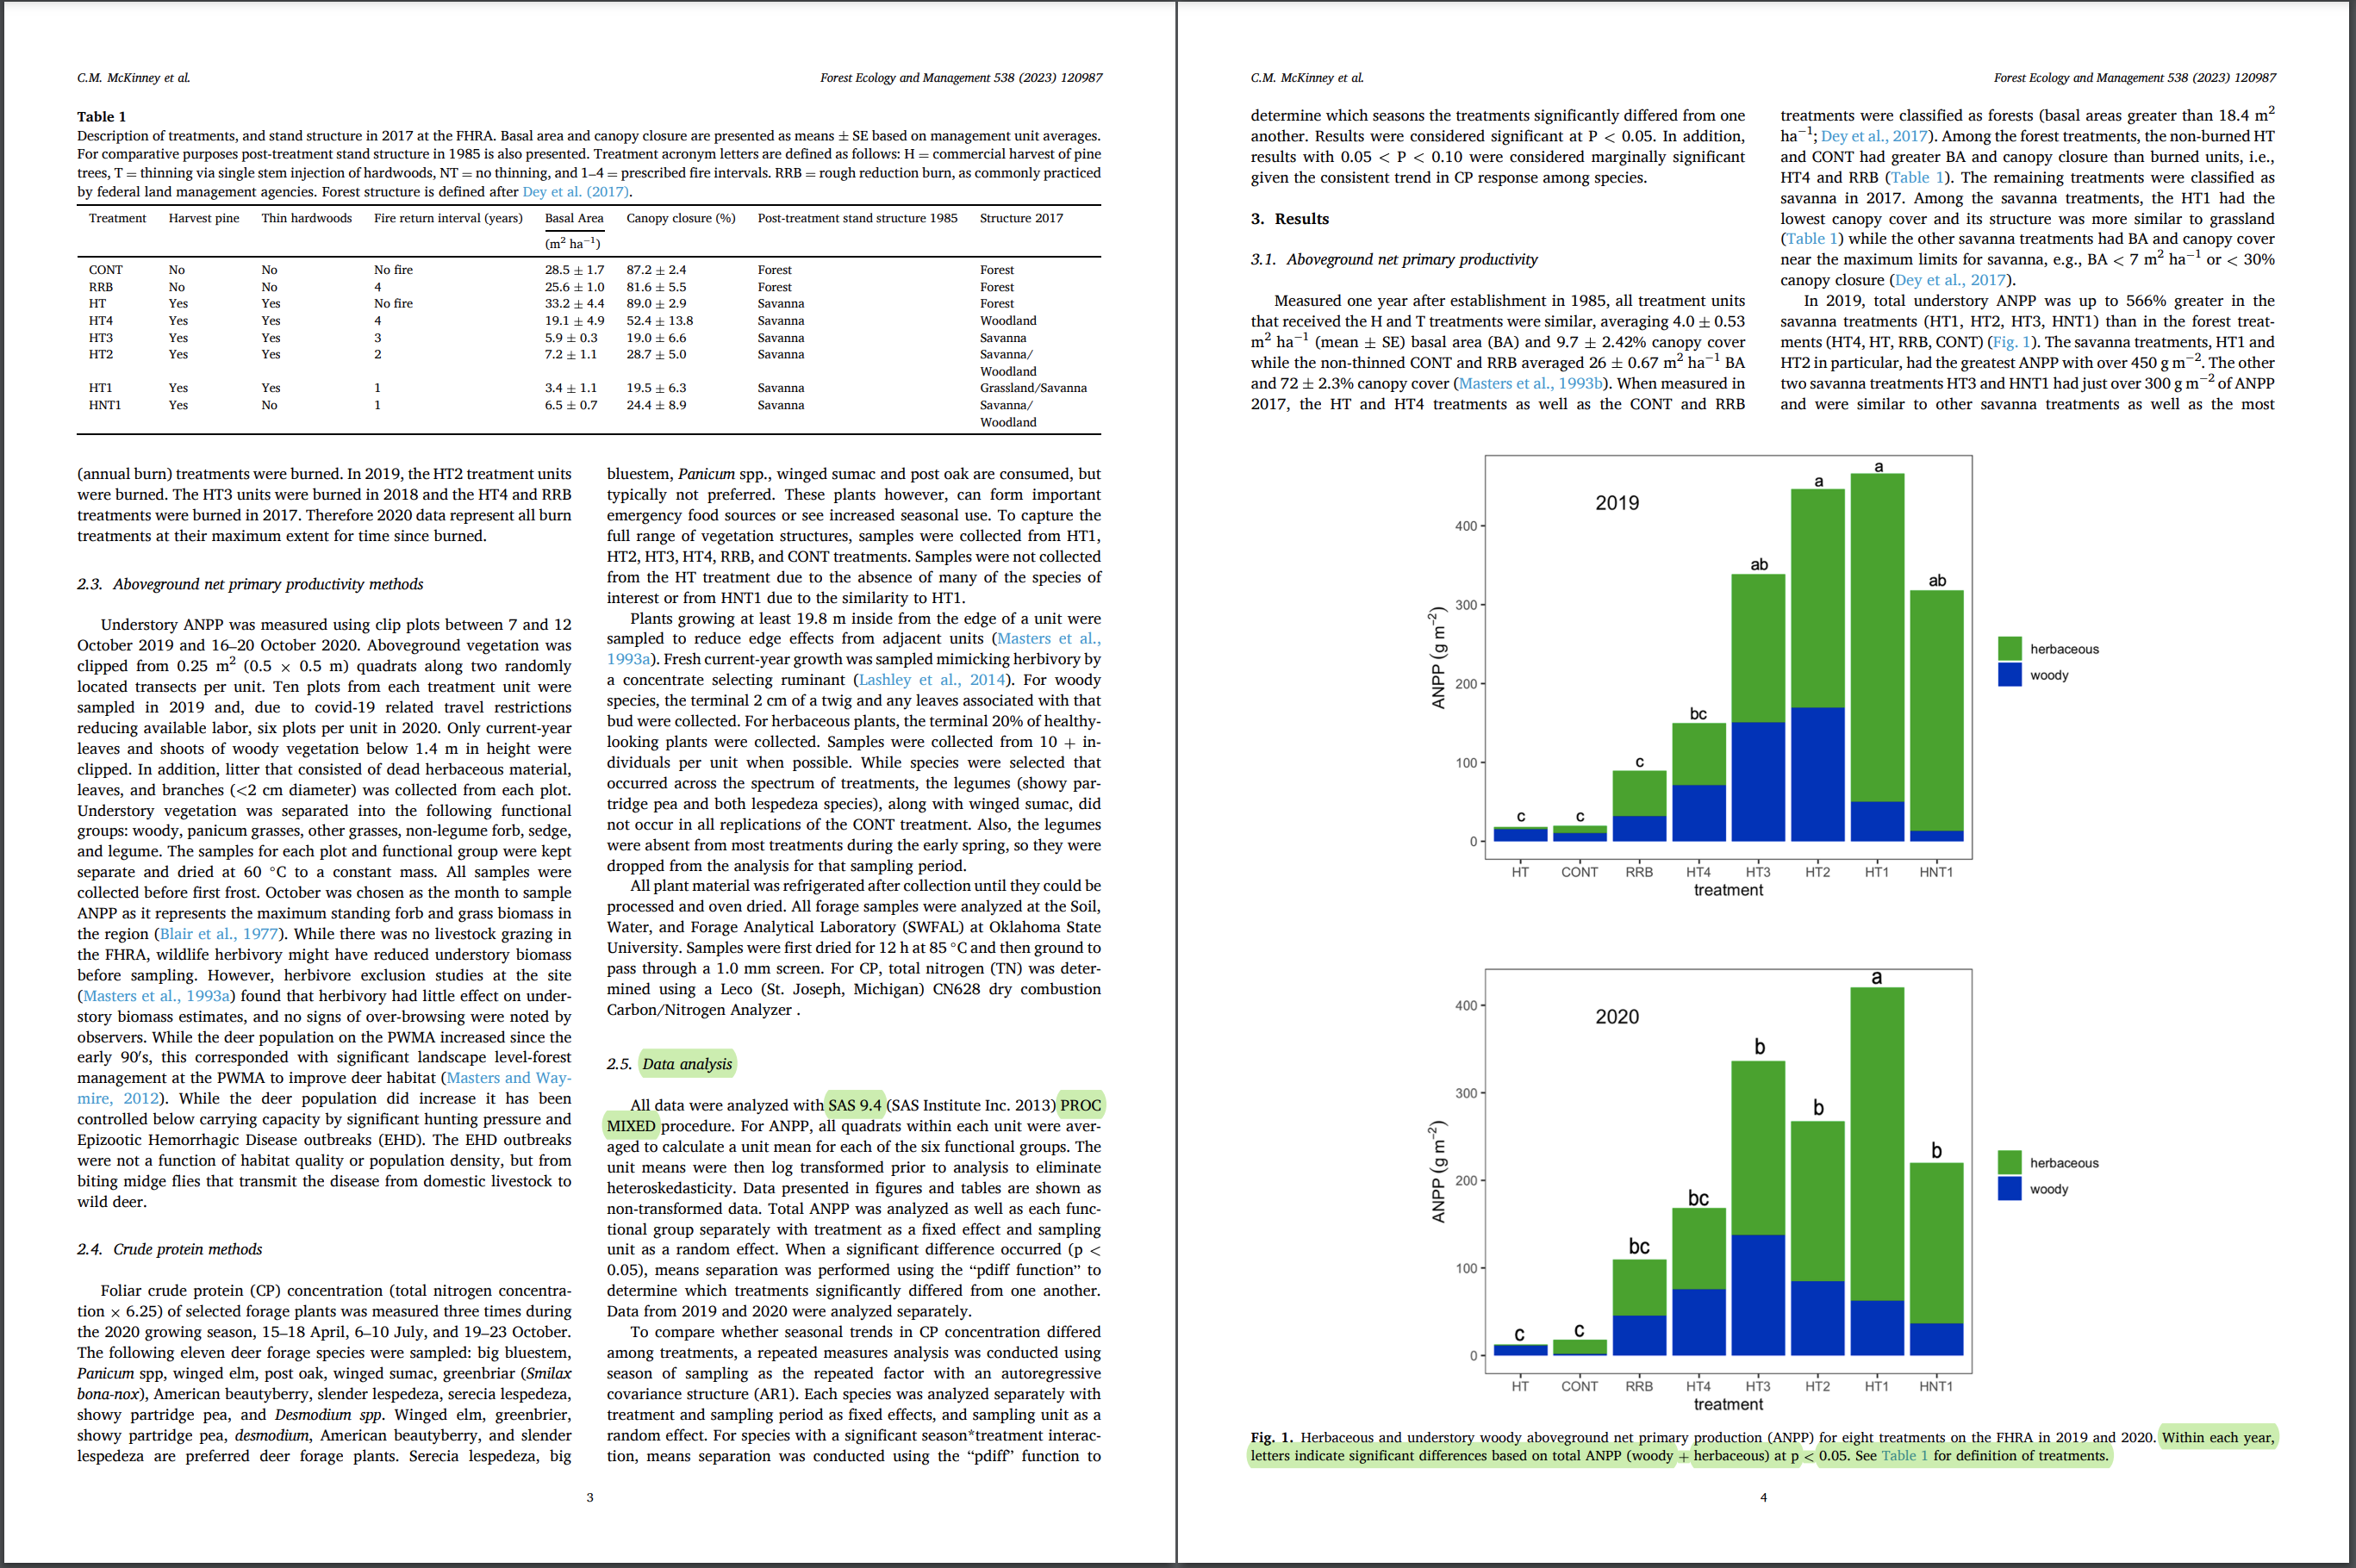
\includegraphics[width = \textwidth, height = 0.95\textheight]{Images/Forest2.png}
\end{frame}

\begin{frame}{}
    \centering 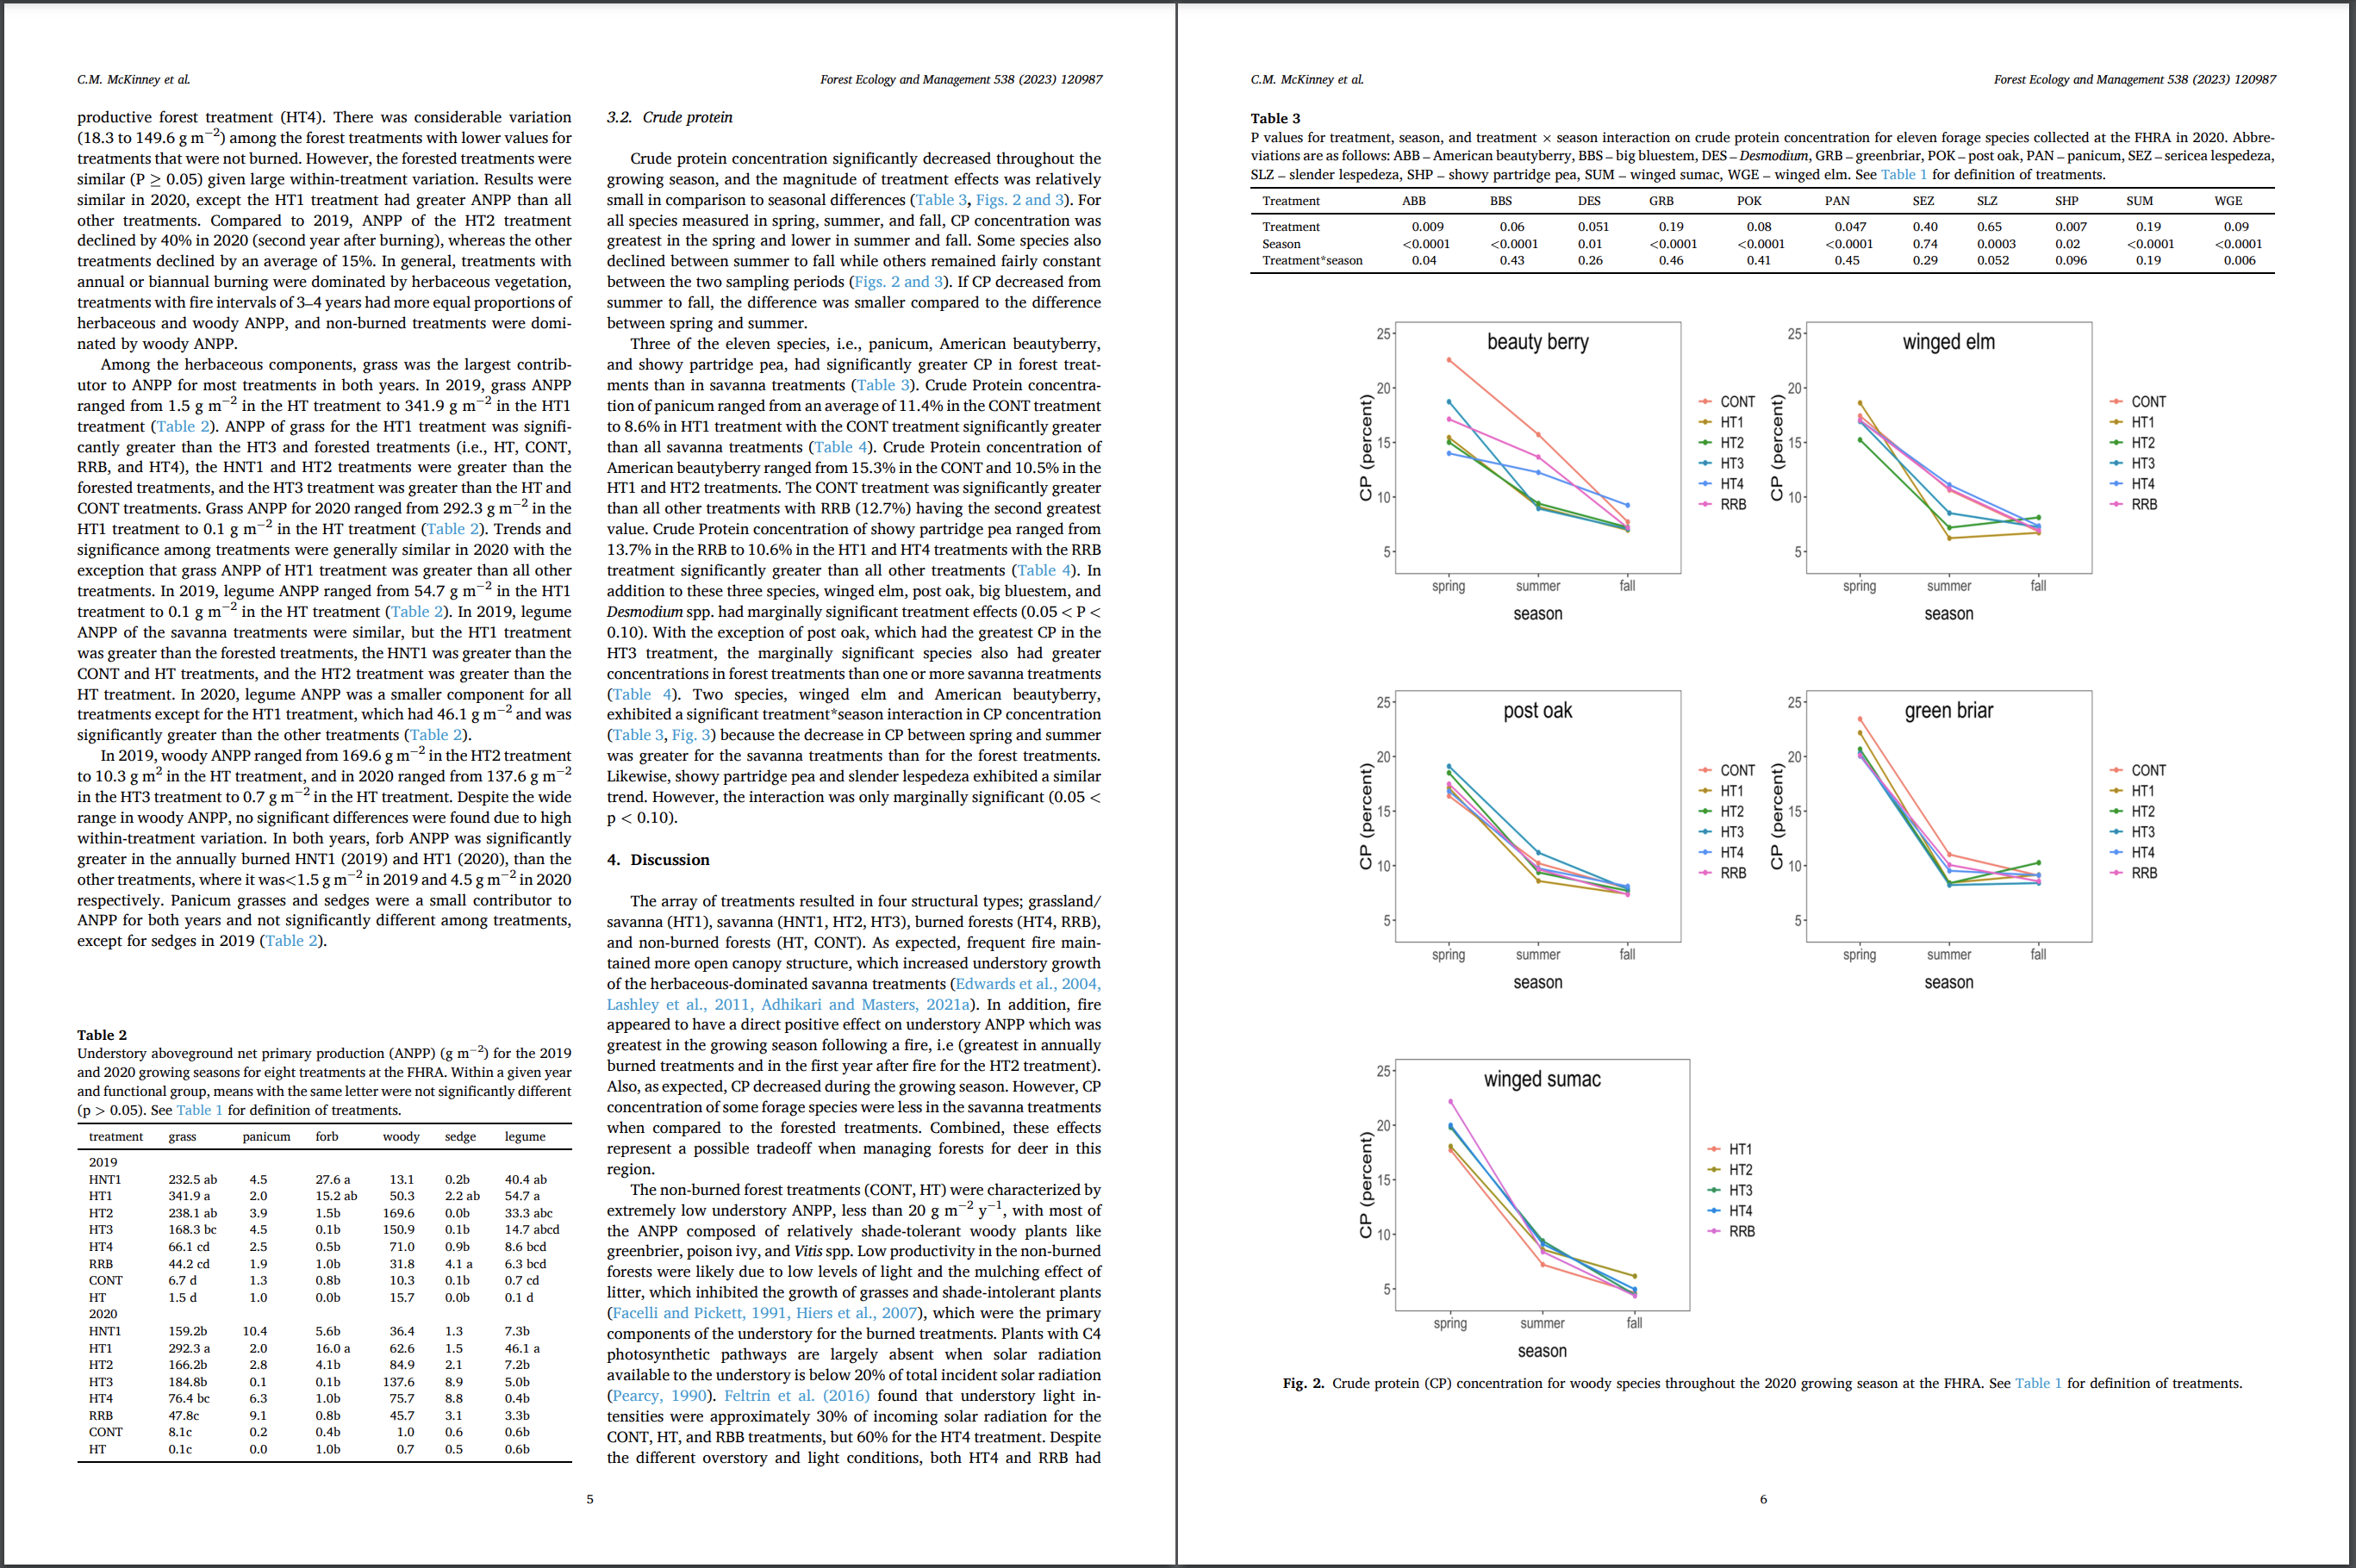
\includegraphics[width = \textwidth, height = 0.95\textheight]{Images/Forest3.png}
\end{frame}

\begin{frame}{}
    \centering 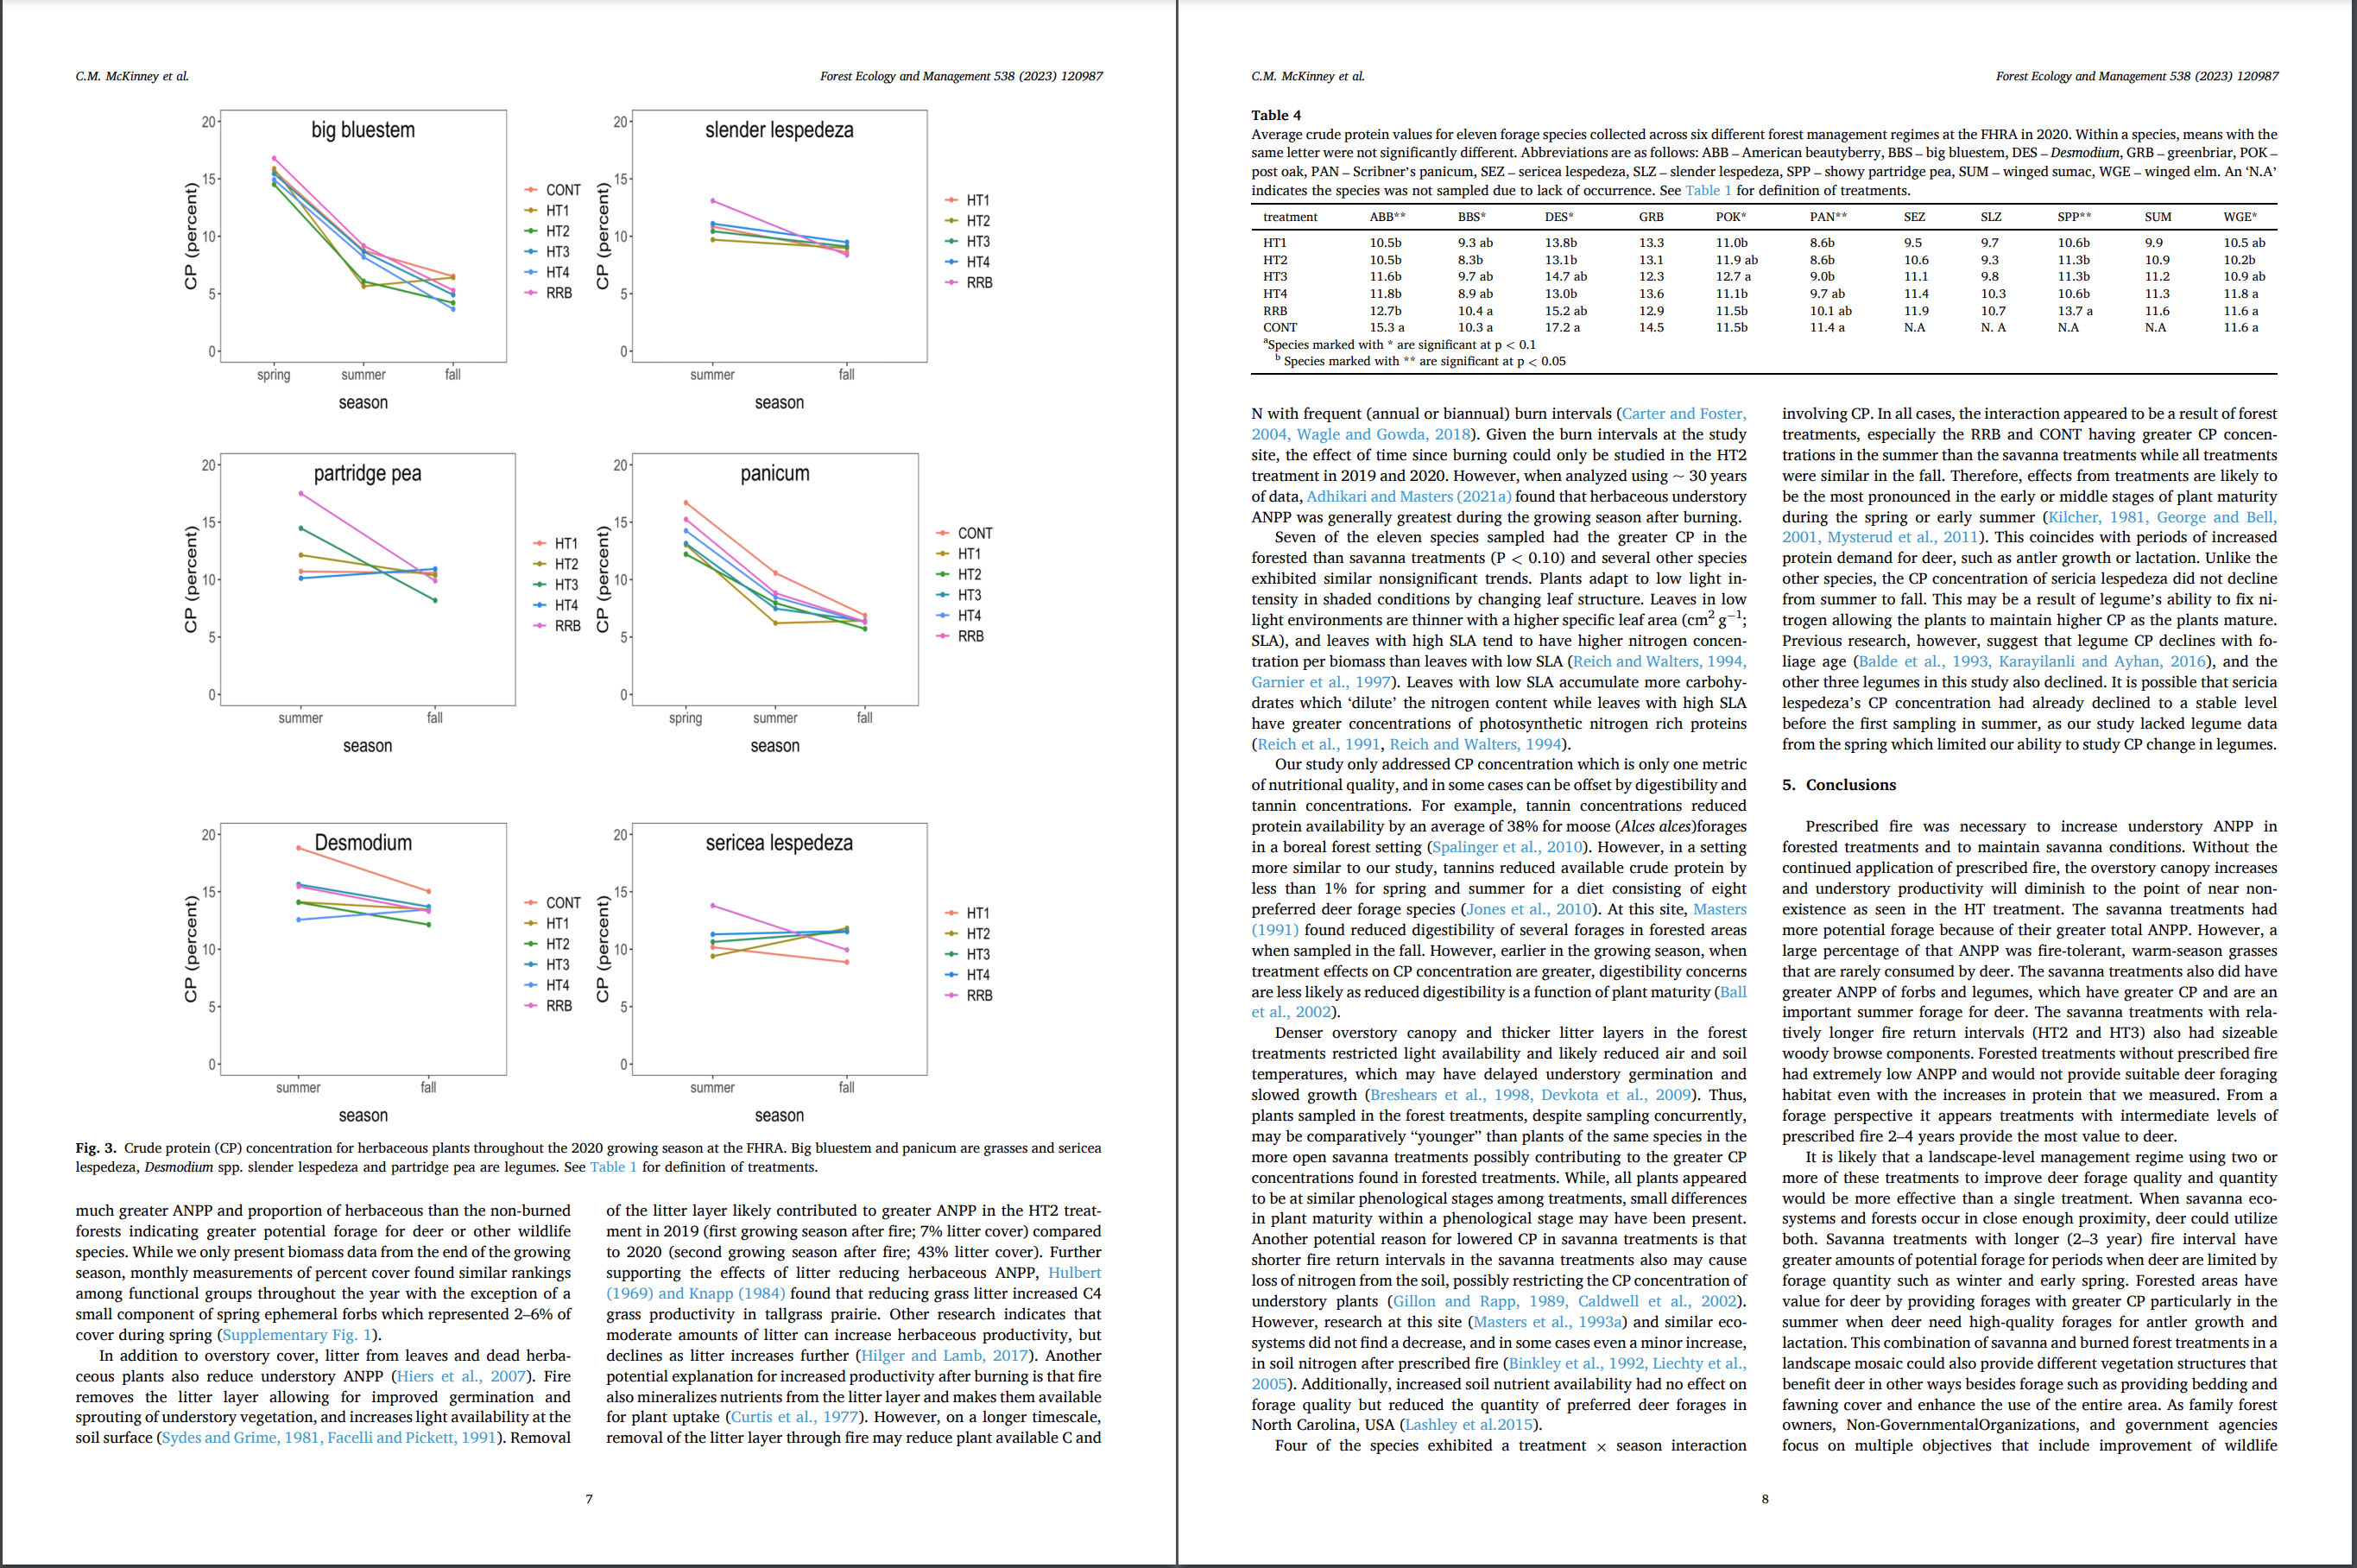
\includegraphics[width = \textwidth, height = 0.95\textheight]{Images/Forest4.png}
\end{frame}

\begin{frame}{}
    \centering 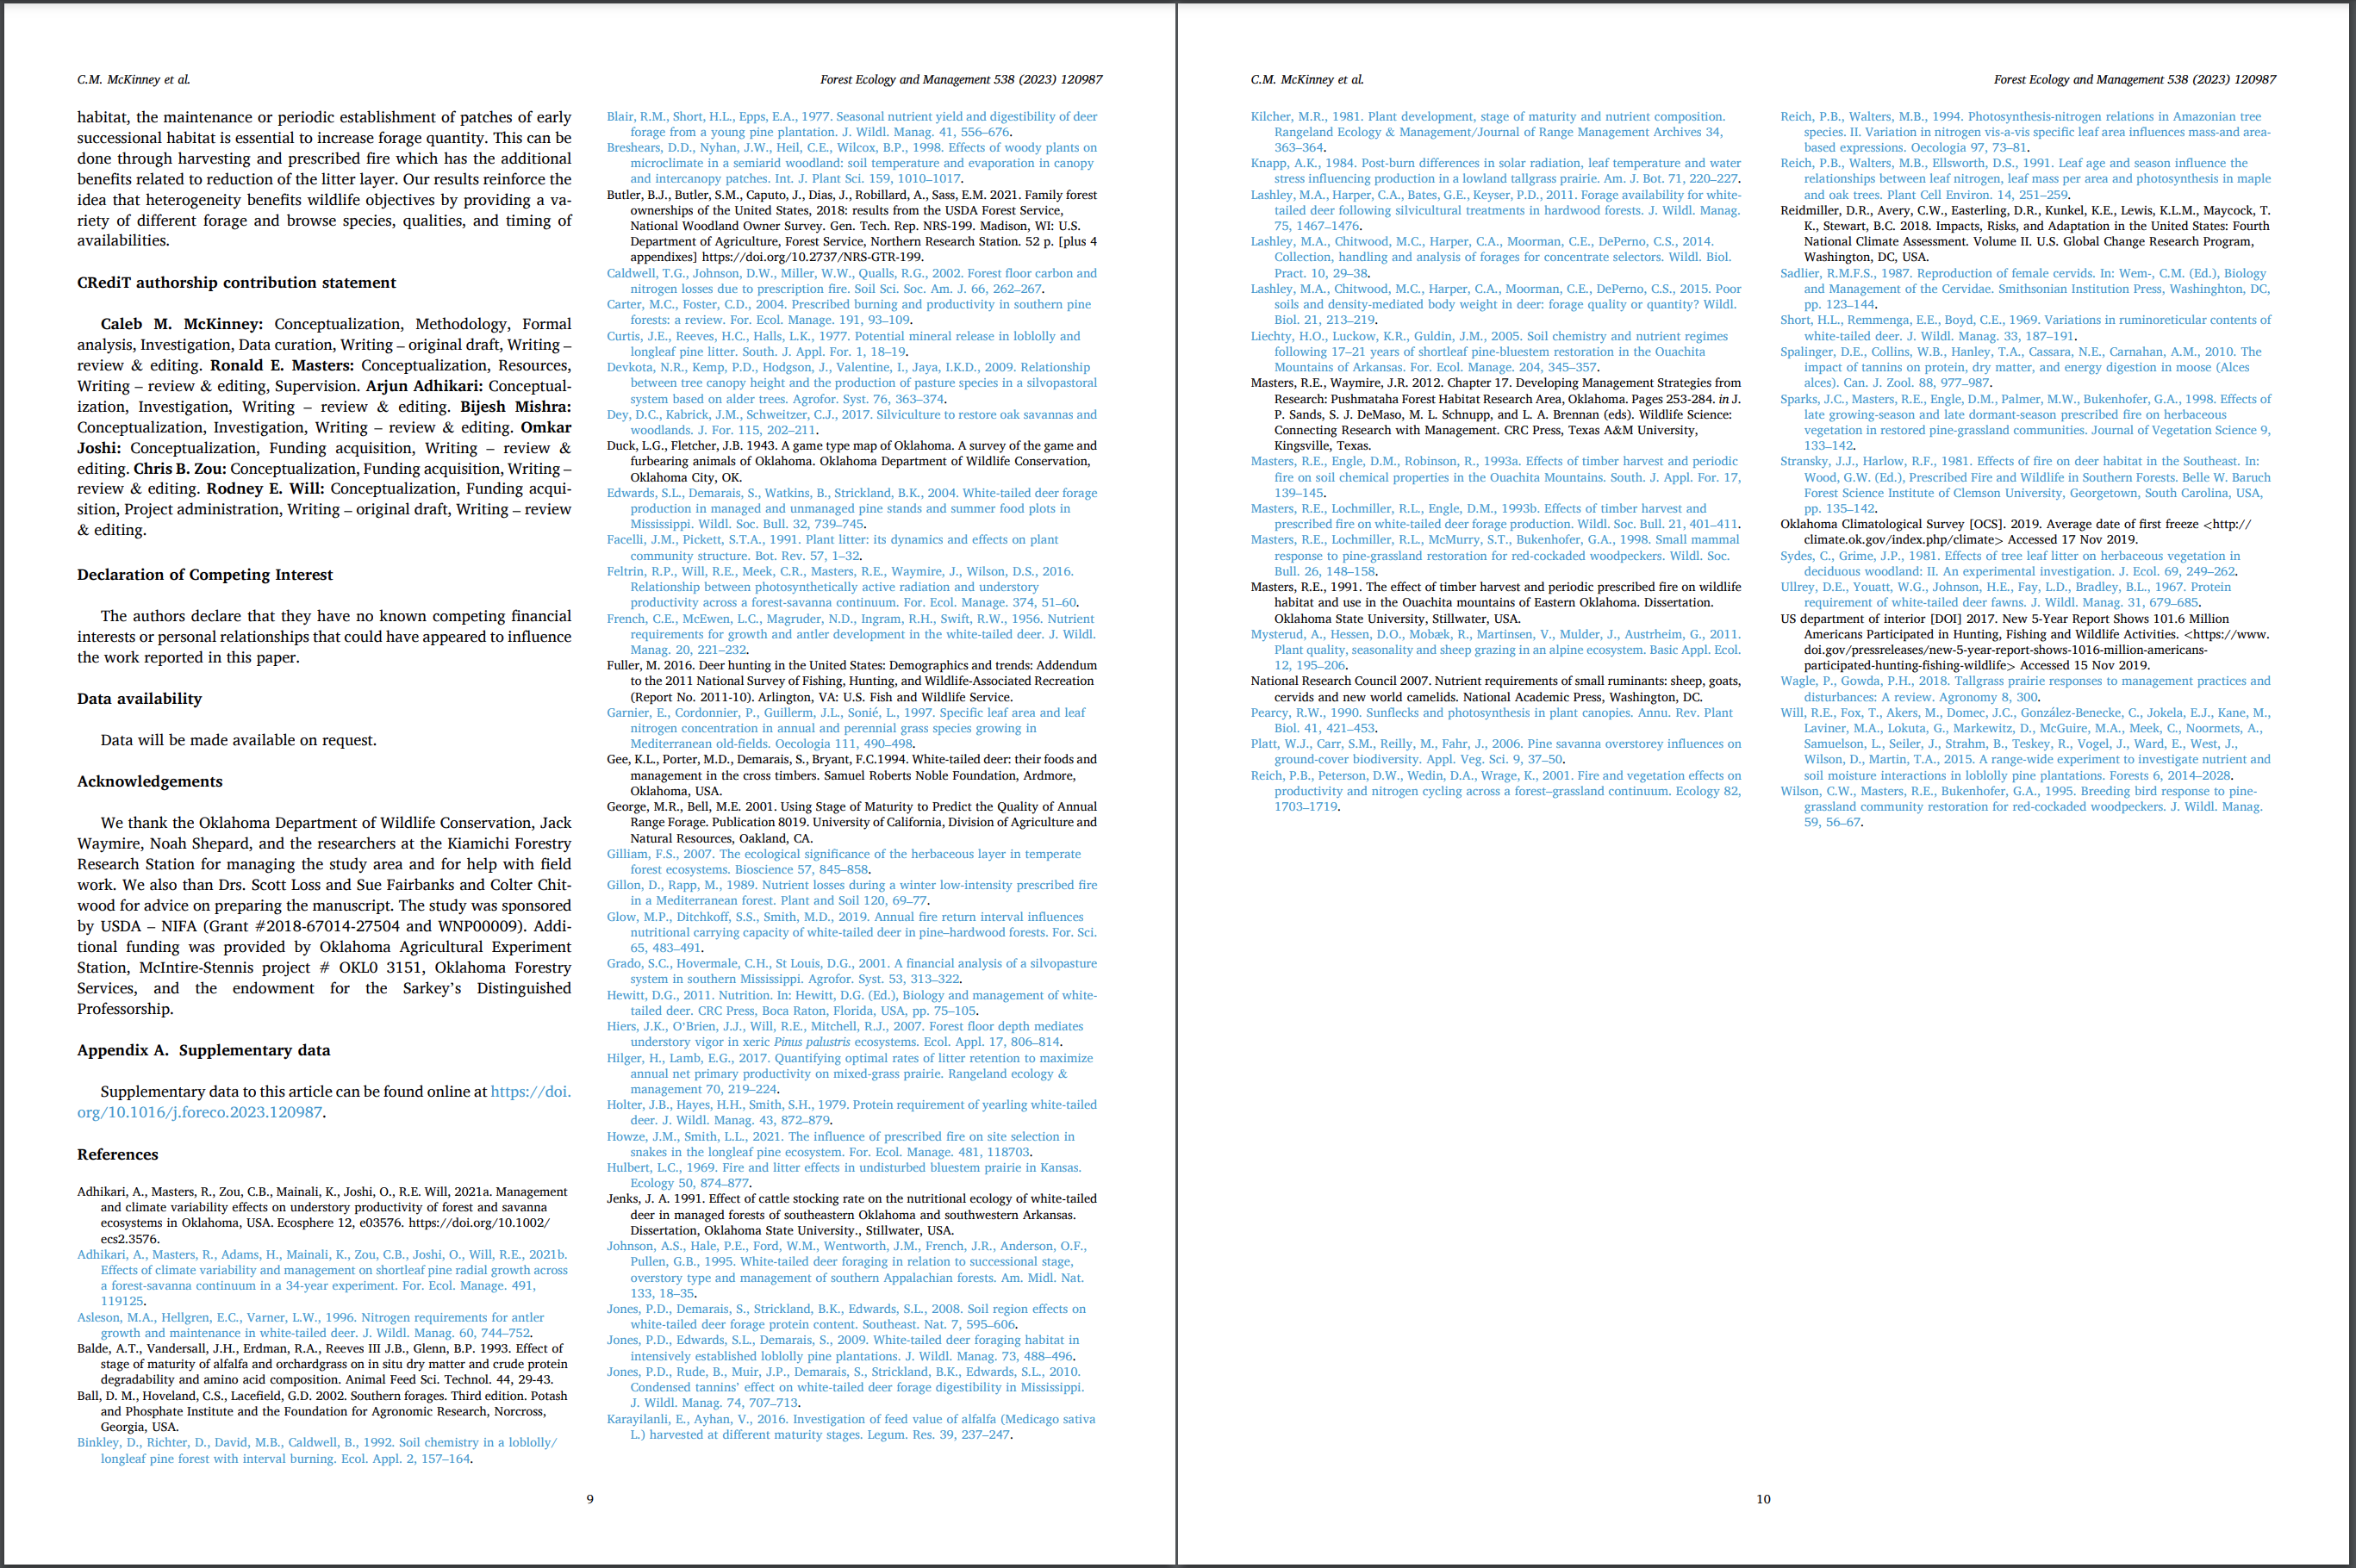
\includegraphics[width = \textwidth, height = 0.95\textheight]{Images/Forest5.png}
\end{frame}

\begin{frame}{}
    \centering 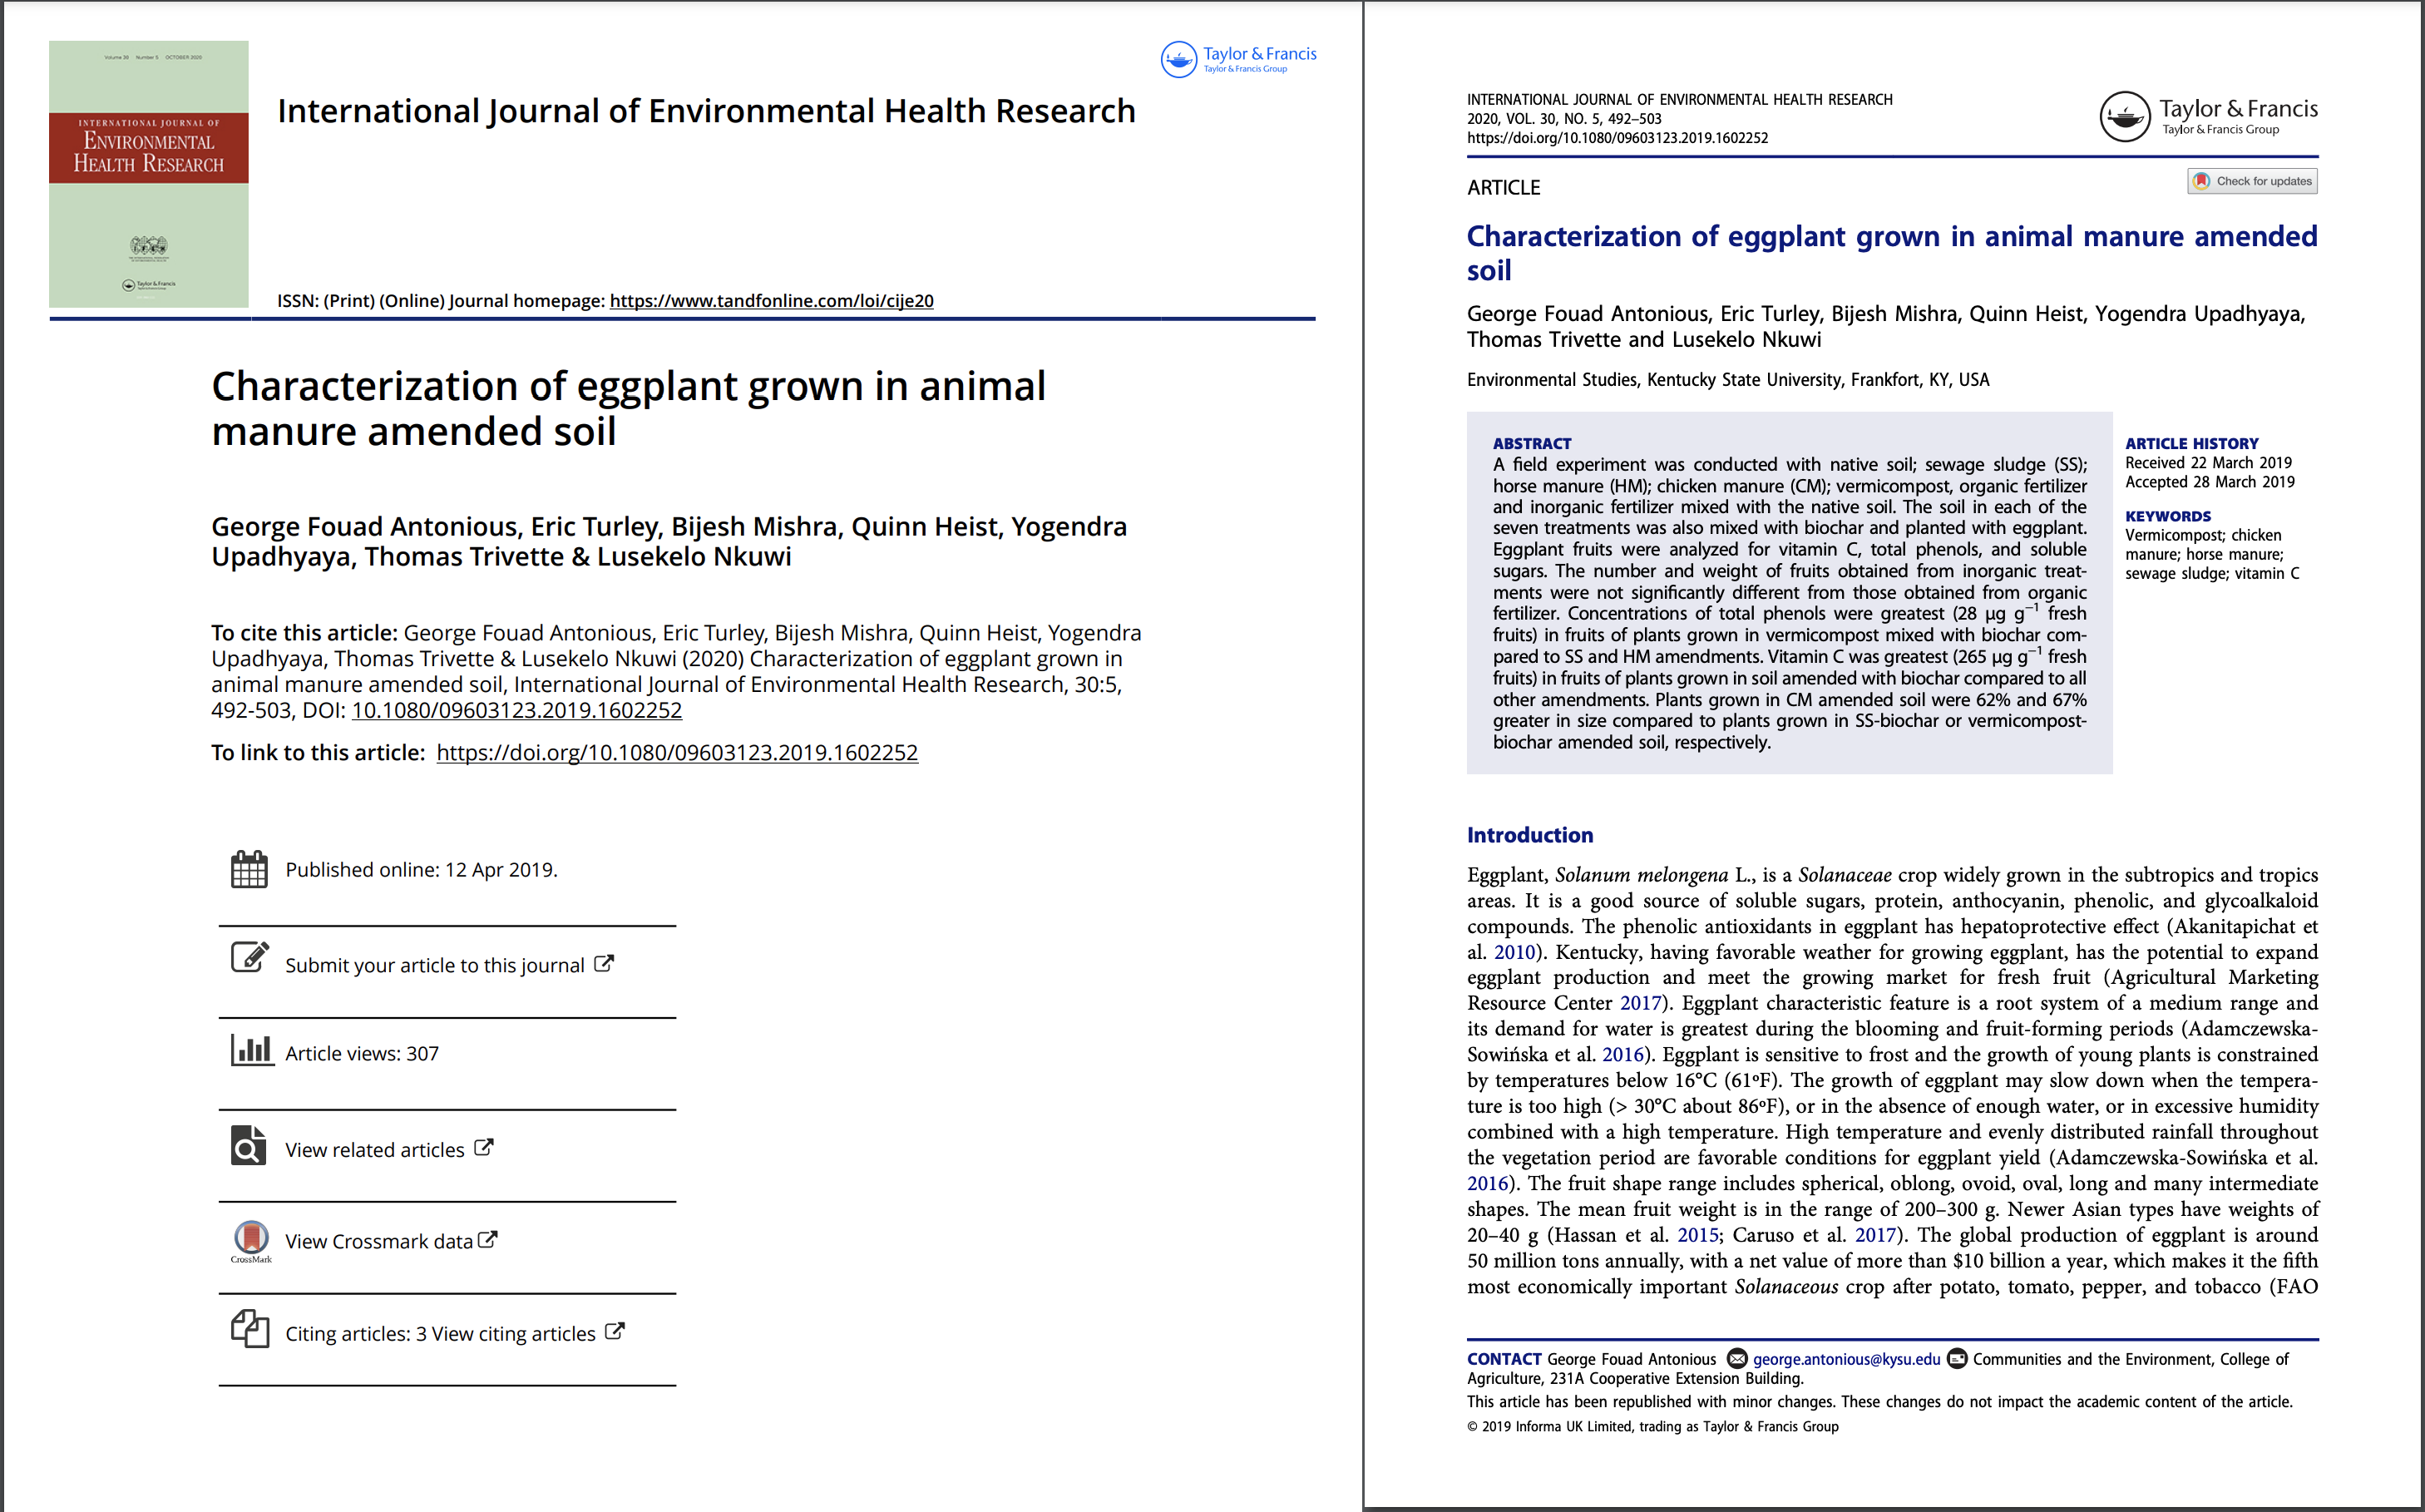
\includegraphics[width = \textwidth, height = 0.95\textheight]{Images/Eggplant1.png}
\end{frame}

\begin{frame}{}
    \centering 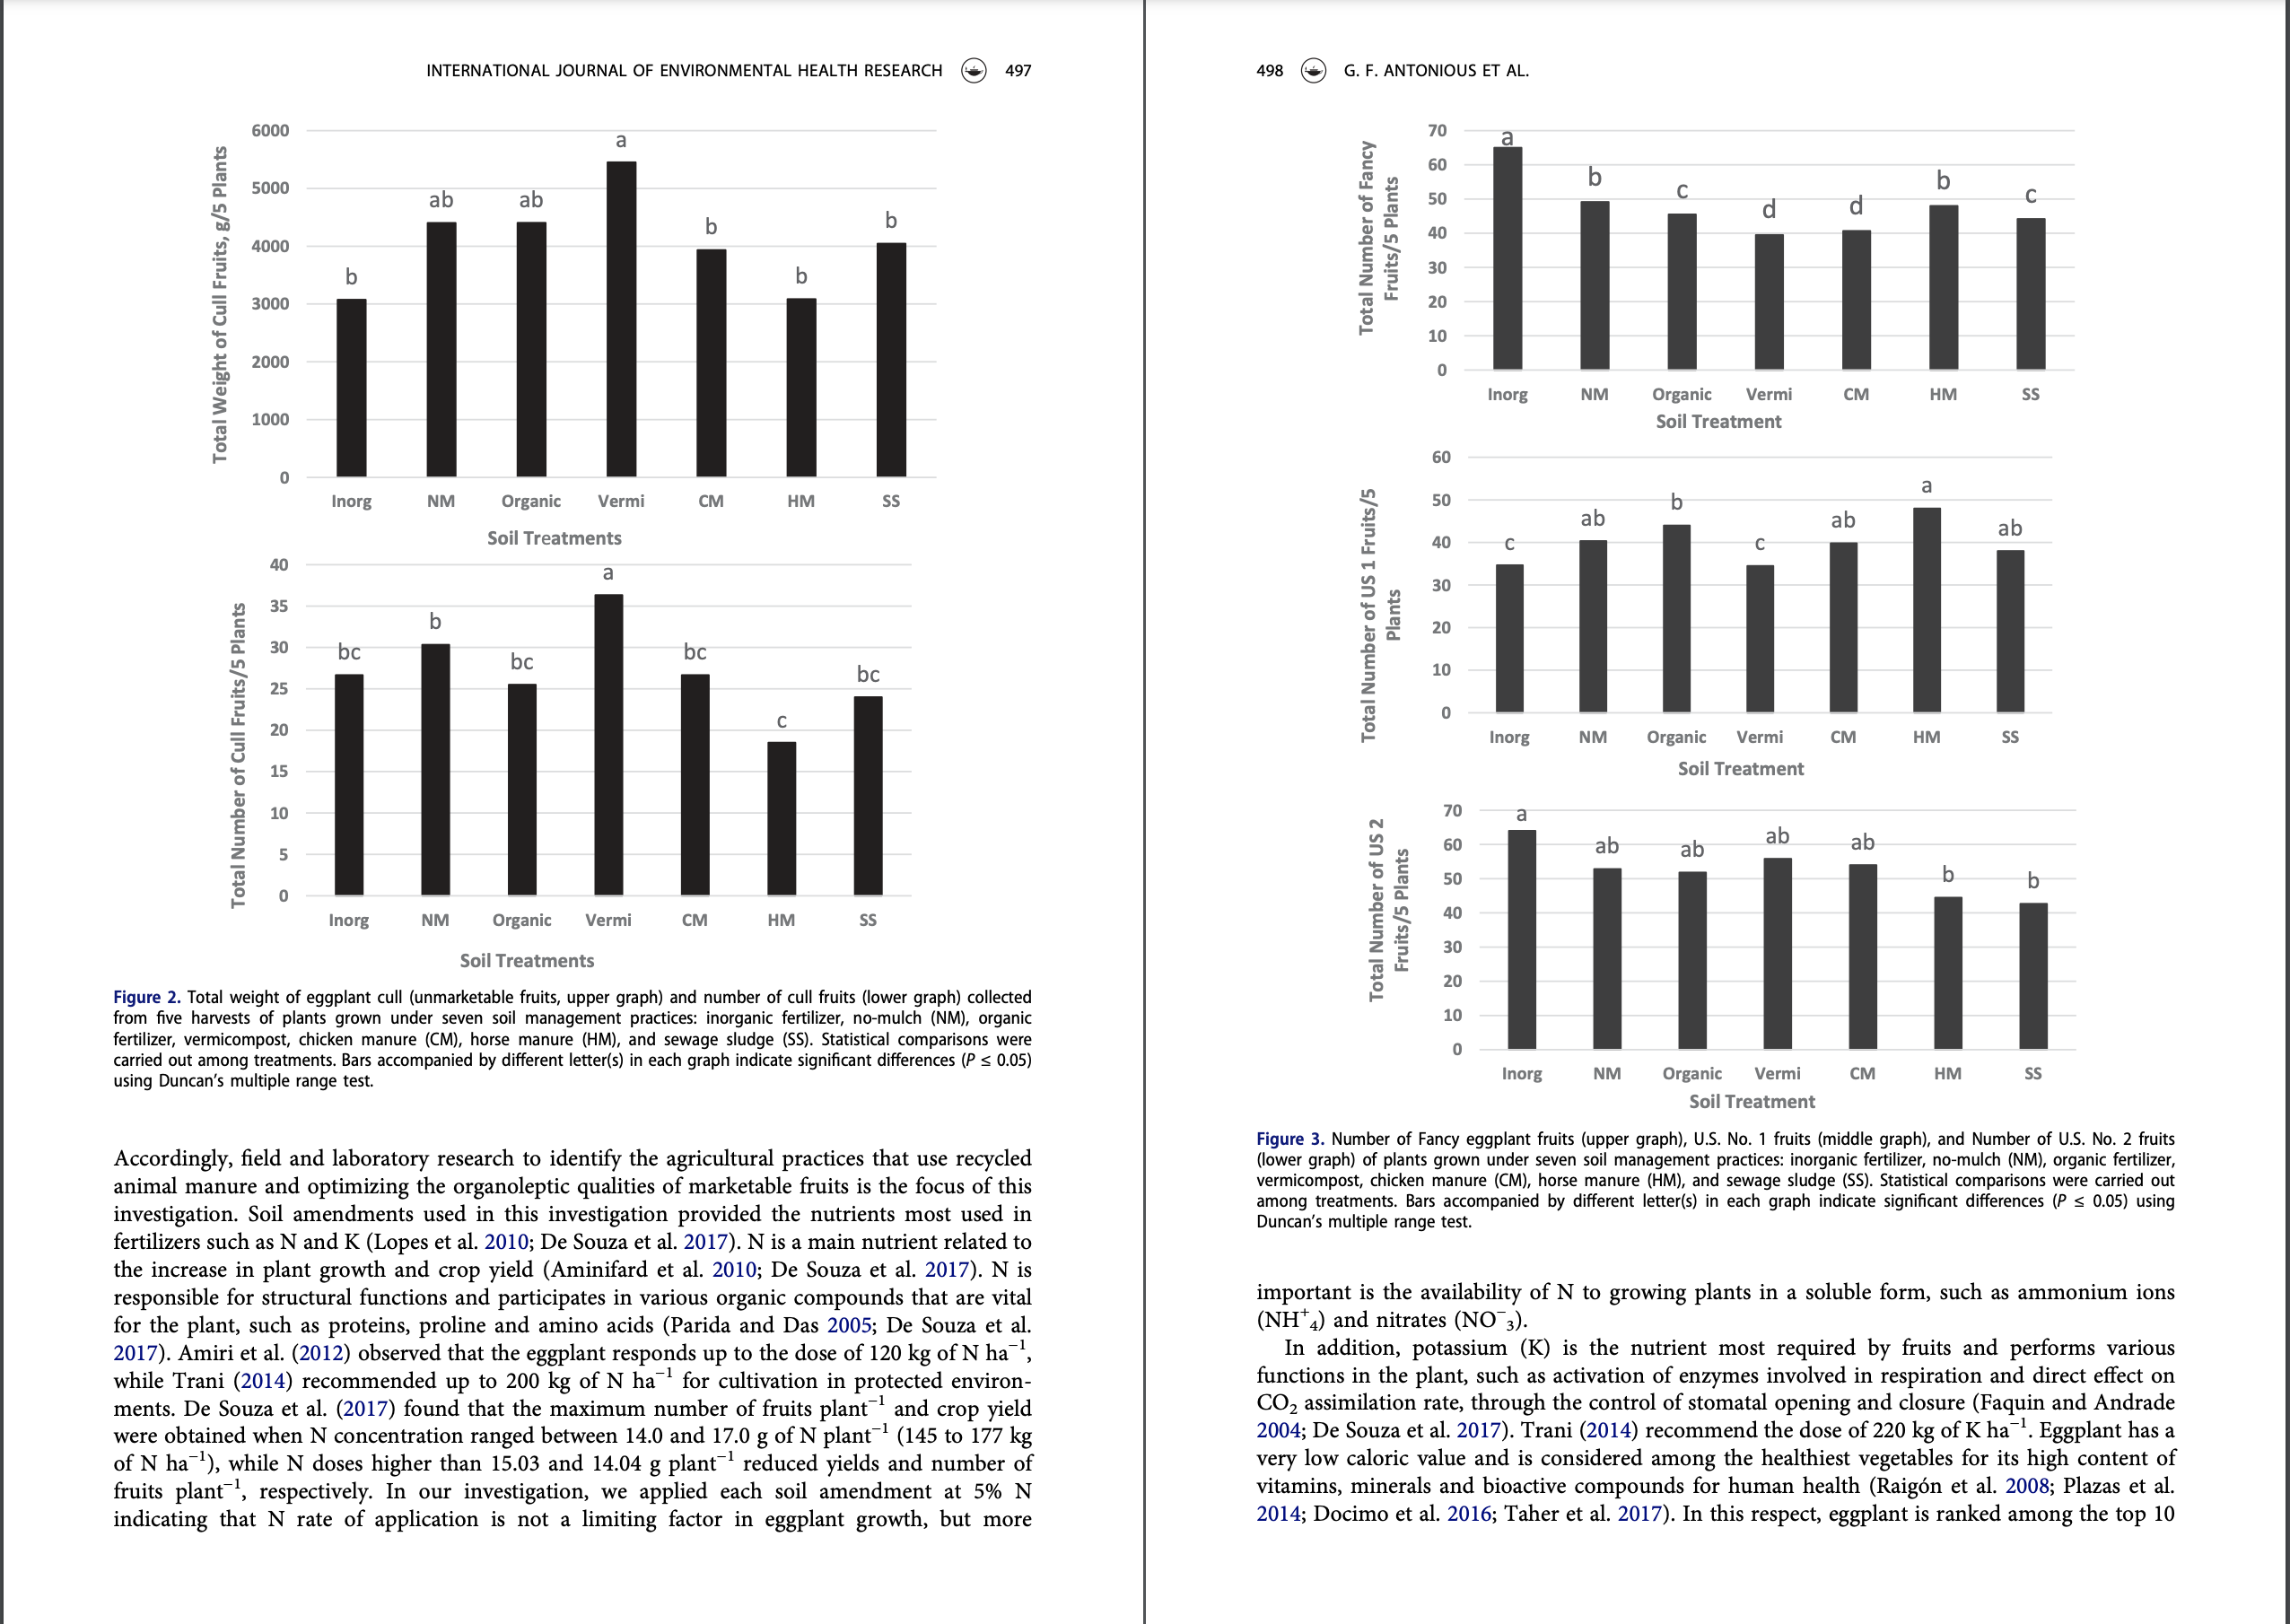
\includegraphics[width = \textwidth, height = 0.95\textheight]{Images/Eggplant2.png}
\end{frame}

\begin{frame}{}
    \centering 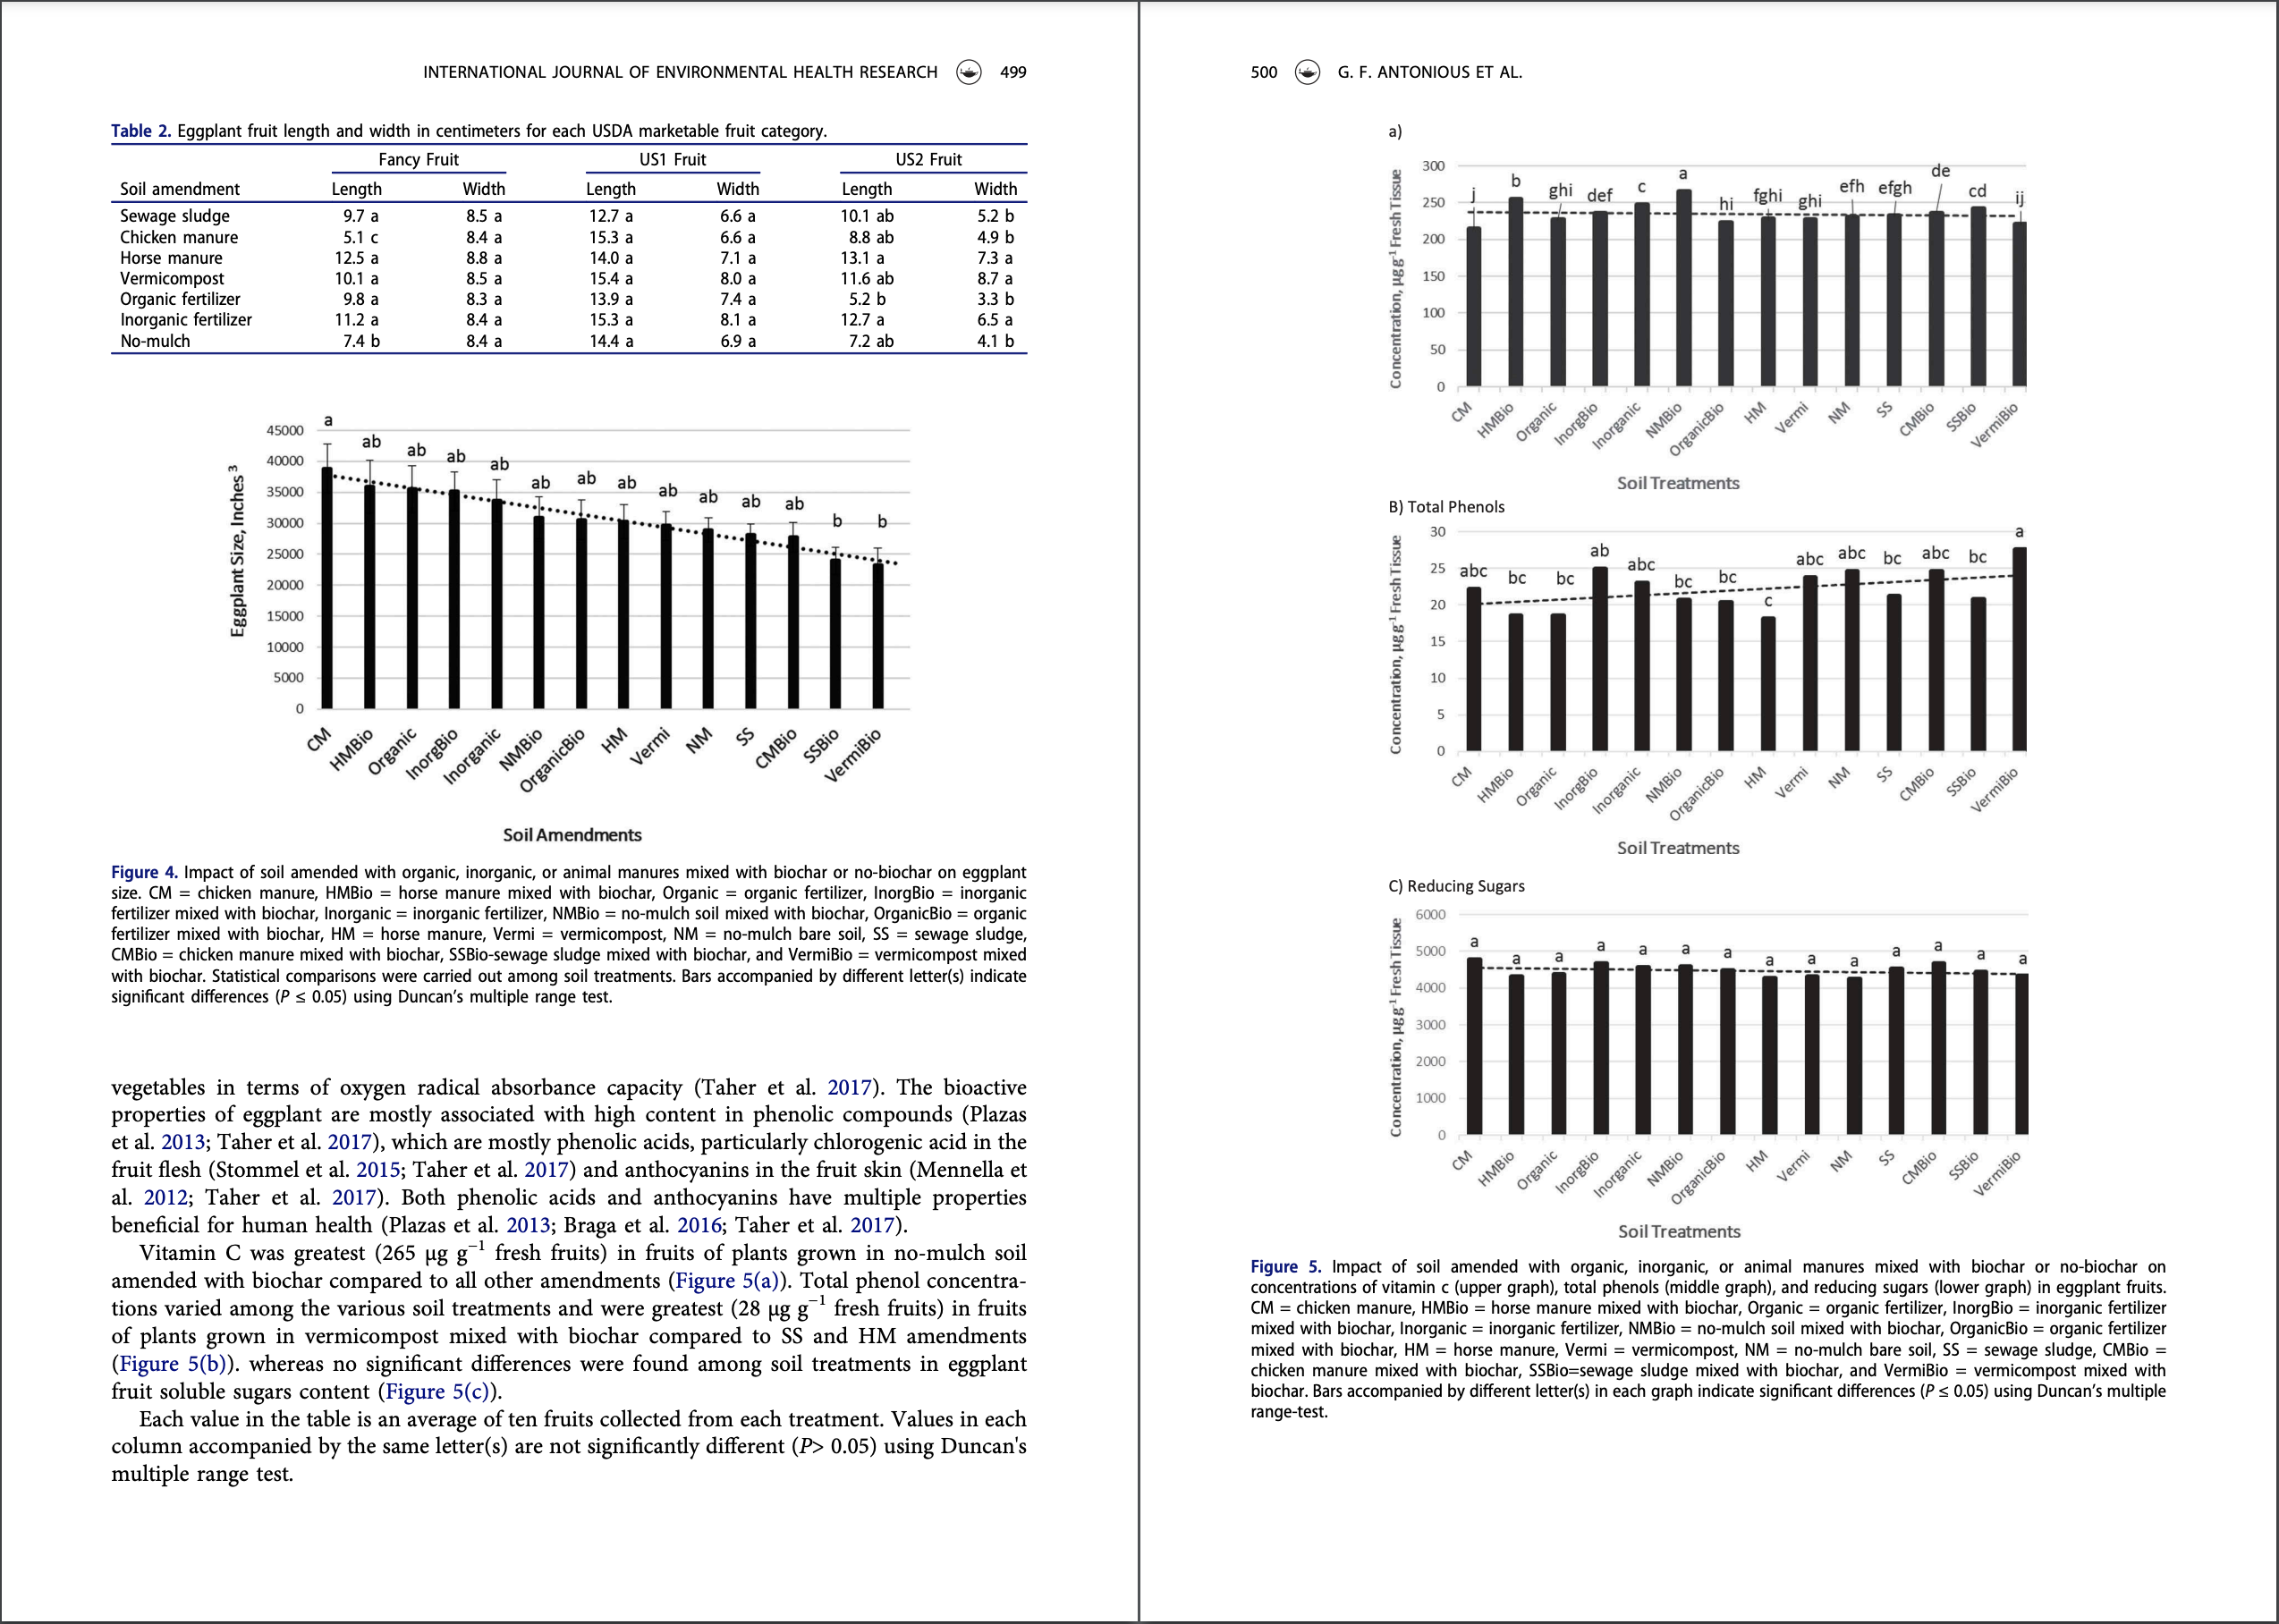
\includegraphics[width = \textwidth, height = 0.95\textheight]{Images/Eggplant3.png}
\end{frame}
%%%%%%%%%%%%%%%%%

\begin{frame}{Some Suggestions for Reading Scientific Papers}
	\begin{itemize}
    \item Some websites to search recent papers: {\color{blue}\href{https://scholar.google.com/}{Google Scholar}}, {\color{blue}\href{https://www.ssrn.com/index.cfm/en/}{SSRN}}, {\color{blue}\href{https://clarivate.libguides.com/directlinks}{Web of Science}}, {\color{blue}\href{https://www.researchsquare.com/}{SCOPUS}}, {\color{blue}\href{https://www.researchsquare.com/}{Research Square}}, {\color{blue}\href{https://arxiv.org/}{arXiv}}, {\color{blue}\href{https://www.preprints.org/}{Preprints}}, {\color{blue}\href{https://ageconsearch.umn.edu/?ln=en}{AgEcon Search}}, {\color{blue}\href{http://repec.org/}{REPEC}}, {\color{blue}\href{https://osf.io/preprints/socarxiv/}{SocArXiv}}, {\color{blue}\href{https://osf.io/preprints/}{OSF Preprints}}, {\color{blue}\href{https://en.wikipedia.org/wiki/List_of_academic_publishers_by_preprint_policy}{Academic publishers with pre-prints policy}}.
    \item Use relevant keywords to find papers in your field.
	\item Know what you want to know (subject matter, background, method, findings, evidences to back up your findings etc.)
    \item Read each line carefully and pay attention to each and every words. Careful reading also helps to identify the quality of paper.
    \item Read multiple papers and multiple times. Almost, every time you will find new information.
	\end{itemize}
\end{frame}
\end{document}